\documentclass[conference]{IEEEtran}
\usepackage{times}

% numbers option provides compact numerical references in the text. 
\usepackage[numbers]{natbib}
\usepackage{multicol}

\usepackage{xspace}
\usepackage[colorlinks=true,linkcolor=blue,citecolor=blue,bookmarks=true]{hyperref}

\usepackage{wrapfig}

\usepackage{graphicx}
\usepackage{subcaption}
\usepackage{booktabs}

\usepackage[skins,theorems]{tcolorbox}

\newcommand{\rebuttal}[1]{\textcolor{red}{#1}}


\pdfinfo{
   /Author (Homer Simpson)
   /Title  (Robots: Our new overlords)
   /CreationDate (D:20101201120000)
   /Subject (Robots)
   /Keywords (Robots;Overlords)
}

%% editing comment
\newcommand{\cmt}[1]{{\footnotesize\textcolor{red}{#1}}}
\newcommand{\cmto}[1]{{\footnotesize\textcolor{orange}{#1}}}
\newcommand{\note}[1]{\cmt{Note: #1}}
\newcommand{\todo}[1]{\cmt{TO-DO: #1}}
\newcommand{\question}[1]{\cmto{Question: #1}}
\newcommand{\sergey}[1]{{\footnotesize\textcolor{blue}{Sergey: #1}}}
\newcommand{\ak}[1]{{\textcolor{black}{#1}}}
\newcommand{\edits}[1]{\textcolor{blue}{#1}}
\newcommand{\editsred}[1]{\textcolor{red}{#1}}
\newcommand{\editsp}[1]{\textcolor{purple}{#1}}
\newcommand{\editsv}[1]{\textcolor{magenta}{#1}}


\newcommand{\methodname}{Cal-QL}
\newcommand{\aliasingproblemname}{bootstrapping aliasing}
\newcommand{\Aliasingproblemname}{Bootstrapping aliasing}
\newcommand{\AliasingProblemName}{Bootstrapping Aliasing}
\newcommand{\simnorm}{\mathrm{sim}_{\mathrm{n}}^\pi}
\newcommand{\simunnorm}{\mathrm{sim}_{\mathrm{u}}^\pi}

%% abbreviations
\newcommand{\x}{\mathbf{x}}
\newcommand{\z}{\mathbf{z}}
\newcommand{\y}{\mathbf{y}}
\newcommand{\w}{\mathbf{w}}
\newcommand{\data}{\mathcal{D}}

\newcommand{\etal}{{et~al.}\ }
\newcommand{\eg}{e.g.\ }
\newcommand{\ie}{i.e.\ }
\newcommand{\nth}{\text{th}}
\newcommand{\pr}{^\prime}
\newcommand{\tr}{^\mathrm{T}}
\newcommand{\inv}{^{-1}}
\newcommand{\pinv}{^{\dagger}}
\newcommand{\real}{\mathbb{R}}
\newcommand{\gauss}{\mathcal{N}}
\newcommand{\norm}[1]{\left|#1\right|}
\newcommand{\trace}{\text{tr}}

%% specifics for the paper
\newcommand{\reward}{r}
\newcommand{\policy}{\pi}
\newcommand{\mdp}{\mathcal{M}}
\newcommand{\states}{\mathcal{S}}
\newcommand{\actions}{\mathcal{A}}
\newcommand{\observations}{\mathcal{O}}
\newcommand{\transitions}{T}
\newcommand{\initstate}{d_0}
\newcommand{\freq}{d}
\newcommand{\obsfunc}{E}
\newcommand{\initial}{\mathcal{I}}
\newcommand{\horizon}{H}
\newcommand{\rewardevent}{R}
\newcommand{\probr}{p_\rewardevent}
\newcommand{\metareward}{\bar{\reward}}
\newcommand{\discount}{\gamma}
\newcommand{\behavior}{{\pi_\beta}}
\newcommand{\bellman}{\mathcal{B}}
\newcommand{\qparams}{\phi}
\newcommand{\qparamset}{\Phi}
\newcommand{\qset}{\mathcal{Q}}
\newcommand{\batch}{B}
\newcommand{\qfeat}{\mathbf{f}}
\newcommand{\Qfeat}{\mathbf{F}}
\newcommand{\hatbehavior}{\hat{\pi}_\beta}

\newcommand{\traj}{\tau}

\newcommand{\pihi}{\pi^{\text{hi}}}
\newcommand{\pilo}{\pi^{\text{lo}}}
\newcommand{\ah}{\mathbf{w}}

\newcommand{\proj}{\Pi}

\newcommand{\loss}{\mathcal{L}}
\newcommand{\eye}{\mathbf{I}}

\newcommand{\model}{\hat{p}}
\newcommand{\mhat}{\hat{\mathcal{M}}}
\newcommand{\mdphat}{\widehat{\mathcal{M}}}
\newcommand{\mdpbar}{\overline{\mathcal{M}}}

\newcommand{\pimix}{\pi_{\text{mix}}}

\newcommand{\pib}{\bar{\pi}}
\newcommand{\epspi}{\epsilon_{\pi}}
\newcommand{\epsmodel}{\epsilon_{m}}

\newcommand{\return}{\mathcal{R}}

%% math
\newcommand{\cY}{\mathcal{Y}}
\newcommand{\cX}{\mathcal{X}}
\newcommand{\en}{\mathcal{E}}
\newcommand{\bu}{\mathbf{u}}
\newcommand{\bv}{\mathbf{v}}
\newcommand{\be}{\mathbf{e}}
\newcommand{\by}{\mathbf{y}}
\newcommand{\bx}{\mathbf{x}}
\newcommand{\bz}{\mathbf{z}}
\newcommand{\bw}{\mathbf{w}}
\newcommand{\bo}{\mathbf{o}}
\newcommand{\bs}{\mathbf{s}}
\newcommand{\ba}{\mathbf{a}}
\newcommand{\bM}{\mathbf{M}}
\newcommand{\ot}{\bo_t}
\newcommand{\st}{\bs_t}
\newcommand{\at}{\ba_t}
\newcommand{\op}{\mathcal{O}}
\newcommand{\opt}{\op_t}
\newcommand{\kl}{D_\text{KL}}
\newcommand{\tv}{D_\text{TV}}
\newcommand{\ent}{\mathcal{H}}
\newcommand{\bG}{\mathbf{G}}
\newcommand{\byk}{\mathbf{y_k}}
\newcommand{\bI}{\mathbf{I}}
\newcommand{\bg}{\mathbf{g}}
\newcommand{\bV}{\mathbf{V}}
\newcommand{\bD}{\mathbf{D}}
\newcommand{\bR}{\mathbf{R}}
\newcommand{\bQ}{\mathbf{Q}}
\newcommand{\bA}{\mathbf{A}}
\newcommand{\bN}{\mathbf{N}}
\newcommand{\bS}{\mathbf{S}}
\newcommand{\bW}{\mathbf{W}}
\newcommand{\bU}{\mathbf{U}}
\newcommand{\bO}{\mathbf{O}}

\newcommand{\bzhi}{\bz^\text{hi}}

\newcommand{\expected}{\mathbb{E}}
\newcommand{\E}{\mathbb{E}}
\newcommand{\srank}{\text{srank}}
\newcommand{\rank}{\text{rank}}
\newcommand{\deepnet}{\bW_N(k, t) \bW_\phi(k, t)}
\newcommand{\features}{\bW_\phi(k, t)}
\newcommand{\stateactioni}{[\bs_i; \ba_i]}
\newcommand{\diag}{\text{\textbf{diag}}}

\def\thetaP{\theta^{\prime}}
\def\cf{\emph{c.f.}\ }
\def\vs{\emph{vs}.\ }
\def\etc{\emph{etc.}\ }
\def\Eqref#1{Equation~\ref{#1}}

\newenvironment{repeatedthm}[1]{\@begintheorem{#1}{\unskip}}{\@endtheorem}
\newcommand{\algname}{COMBO\xspace}

\newtheorem{theorem}{Theorem}[section]
\newtheorem{sketchtheorem}{Sketch Theorem}[section]
\newtheorem{lemma}[theorem]{Lemma}
\newtheorem{corollary}[theorem]{Corollary}
\newtheorem{proposition}[theorem]{Proposition}
\newtheorem{definition}[theorem]{Definition}
\newtheorem{conjecture}[theorem]{Conjecture}
\newtheorem{problem}[theorem]{Problem}
\newtheorem{formulation}[theorem]{Formulation}
\newtheorem{claim}[theorem]{Claim}
\newtheorem{remark}[theorem]{Remark}
\newtheorem{example}[theorem]{Example}
\newtheorem{assumption}[theorem]{Assumption}
\newtheorem{exercise}[theorem]{Exercise}


\newcommand{\indep}{\rotatebox[origin=c]{90}{$\models$}}

\renewcommand{\mathbf}{\boldsymbol}

\newcommand{\conv}{\circledast}
\newcommand{\mb}{\mathbf}
\newcommand{\mc}{\mathcal}
\newcommand{\mf}{\mathfrak}
\newcommand{\md}{\mathds}
\newcommand{\bb}{\mathbb}
\newcommand{\msf}{\mathsf}
\newcommand{\mcr}{\mathscr}
\newcommand{\magnitude}[1]{ \left| #1 \right| }
\newcommand{\set}[1]{\left\{ #1 \right\}}
\newcommand{\condset}[2]{ \left\{ #1 \;\middle|\; #2 \right\} }


\newcommand{\reals}{\bb R}
\newcommand{\proj}{\mathrm{proj}}

\newcommand{\eps}{\varepsilon}
\newcommand{\R}{\reals}
\newcommand{\Cp}{\bb C}
\newcommand{\Z}{\bb Z}
\newcommand{\N}{\bb N}
\newcommand{\Sp}{\bb S}
\newcommand{\Ba}{\bb B}
\newcommand{\indicator}[1]{\mathbbm 1\left\{#1\right\}}
\renewcommand{\P}{\mathbb{P}}
\newcommand{\rvline}{\hspace*{-\arraycolsep}\vline\hspace*{-\arraycolsep}}
\makeatletter
\def\Ddots{\mathinner{\mkern1mu\raise\p@
\vbox{\kern7\p@\hbox{.}}\mkern2mu
\raise4\p@\hbox{.}\mkern2mu\raise7\p@\hbox{.}\mkern1mu}}
\makeatother
% to declare new operator
% \DeclareMathOperator{\xxx}{xxx}

%% Other definitions

\newcommand{\event}{\mc E}

\newcommand{\e}{\mathrm{e}}
\newcommand{\im}{\mathrm{i}}
\newcommand{\rconcave}{r_\fgecap}
\newcommand{\Lconcave}{\mc L^\fgecap}
\newcommand{\rconvex}{r_\fgecup}
\newcommand{\Rconvex}{R_\fgecup}
\newcommand{\Lconvex}{\mc L^\fgecup}

\newcommand{\wh}{\widehat}
\newcommand{\wt}{\widetilde}
\newcommand{\ol}{\overline}


\newcommand{\betaconcave}{\beta_\fgecap}
\newcommand{\betagrad}{\beta_{\mathrm{grad}}}

\newcommand{\norm}[2]{\left\| #1 \right\|_{#2}}
\newcommand{\abs}[1]{\left| #1 \right|}
\newcommand{\row}[1]{\text{row}\left( #1 \right)}
\newcommand{\innerprod}[2]{\left\langle #1,  #2 \right\rangle}
\newcommand{\prob}[1]{\bb P\left[ #1 \right]}
\newcommand{\expect}[1]{\bb E\left[ #1 \right]}
\newcommand{\function}[2]{#1 \left(#2\right}
\newcommand{\integral}[4]{\int_{#1}^{#2}\; #3\; #4}
\newcommand{\paren}[1]{\left( #1 \right)}
\newcommand{\brac}[1]{\left[ #1 \right]}
\newcommand{\Brac}[1]{\left\{ #1 \right\}}

% Adding new defs here
\newcommand{\moff}{m_\mr{off}}
\newcommand{\mon}{m_\mr{on}}
\newcommand{\EmpiricalOffline}{\wh{\bb E}_{\mc D^\nu_h}}
\newcommand{\EmpiricalOnline}{\wh{\bb E}_{\mc D^\tau_h}}
\newcommand{\Deltaoff}{\Delta_\mr{off}}
\newcommand{\Deltaon}{\Delta_\mr{on}}
\newcommand{\Vmax}{V_{\max}}
\newcommand{\regret}{\mr{Reg}}
\newcommand{\regreton}{\mr{Sub}_{\mr {on}}}
\newcommand{\regretoff}{\mr{Sub}_{\mr {off}}}
\newcommand{\Doff}{\mc D_\mr{off}}
\newcommand{\Don}{\mc D_\mr{on}}
\newcommand{\piref}{\pi_\mr{ref}}

\newcommand{\nt}[1]{{\color{purple}{\bf [Next: #1]}}}
\newcommand{\here}{{\color{purple}{\bf [Writing here]}}}
% \newcommand{\todo}{{\color{purple}{\bf [TODO]}}}
\newcommand{\sz}[1]{{\color{blue}{\bf [Simon: #1]}}}
% \newcommand{\note}[1]{{\color{red}{\bf [note: #1]}}}
\newcommand{\mr}{\mathrm}
\newcommand{\sym}{\mathrm{Sym}}
\newcommand{\sks}{\mathrm{Skew}}
\newcommand{\inprod}[2]{\langle#1,#2\rangle}
\newcommand{\parans}[1]{\left(#1\right}
\newcommand{\clip}{\msf{clipped}}
\newcommand{\beha}{\msf b}
\numberwithin{equation}{section}

% \def \endprf{\hfill {\vrule height6pt width6pt depth0pt}\medskip}

\newcommand{\cdsmethodname}{CDS}
\newcommand{\udsmethodname}{UDS}
\newcommand{\ptrmethodname}{PTR~}
\newcommand{\primemethodname}{PRIME~}
\newcommand{\arxiv}[1] {{\color{black} #1}}

% \newenvironment{proof}{\noindent {\bf Proof} }{\endprf\par}

% \newcommand{\qed}{{\unskip\nobreak\hfil\penalty50\hskip2em\vadjust{}
%            \nobreak\hfil$\Box$\parfillskip=0pt\finalhyphendemerits=0\par}}


\newcommand\myworries[1]{\textcolor{red}{#1}}
\newcommand\running[1]{\textcolor{blue}{#1}}

\newcommand{\benchl}[1]{{\scriptsize\textsf{#1}}\normalsize\xspace}
\newcommand{\bench}[1]{{\fontsize{8.5}{10}\selectfont\textsf{#1}}\normalsize\xspace}
\newcommand{\code}[1]{{\fontsize{8.5}{1}\selectfont{\tt #1}}\xspace}
\newcommand{\codebold}[1]{{\fontsize{8.5}{1}\selectfont{\tt \textbf{#1}}}\xspace}
\newcommand{\xx}[1]{\textcolor{black}{#1}}
\newcommand{\xxs}[1]{\textcolor{black}{\scriptsize\textsf{#1}}}
\newcommand{\supertiny}[1]{\fontsize{5}{4}\selectfont{#1}}
\newcommand{\xxred}[1]{\textcolor{red}{\textsf{#1}}}
% \DeclareMathOperator{\EX}{\mathbb{\hat{E}}}% expected value
% \makeatletter
% \newcommand\footnoteref[1]{\protected@xdef\@thefnmark{\ref{#1}}\@footnotemark}
% \makeatother
% \usepackage{scrextend}

% \deffootnote[1em]{1em}{1em}{\textsuperscript{\thefootnotemark}\,}
% \newcolumntype{P}[1]{>{\centering\arraybackslash}p{#1}}
% \newcommand\mycommfont[1]{\footnotesize\ttfamily\textcolor{blue}{#1}}

\newcommand\aviral[1]{\textcolor{red}{aviralkumar@: #1}}
\newcommand\ayazdan[1]{\textcolor{red}{ayazdan@: #1}}
\newcommand\sv[1]{\textcolor{red}{SV@: #1}}
\newcommand\fix[1]{\textcolor{green}{#1}}

\newcommand{\round}[1]{\ensuremath{\lfloor#1\rceil}}

\newcommand{\tgray}[1]{\colorbox{lightgray}{\textbf{#1}}}
\newcommand{\finalcheck}[1]{\textcolor{green}{#1}}

\newcommand{\review}[1]{#1}

\newcommand{\niparagraph}[1]{\vspace{2pt}\noindent\textbf{#1}}


\tcbset{
  aibox/.style={
    width=\textwidth,
    top=0pt, bottom=0pt, left=5pt, right=5pt,
    colback=black!6!white,
    colframe=black,
    colbacktitle=brown,
    enhanced,
    center,
    attach boxed title to top left={yshift=-0.1in,xshift=0.15in},
    boxed title style={boxrule=0pt,colframe=black,},
  }
}
\newtcolorbox{AIbox}[2][]{aibox,title=#2,#1}
%%%%% NEW MATH DEFINITIONS %%%%%

\usepackage{amsmath,amsfonts,bm}

% Mark sections of captions for referring to divisions of figures
\newcommand{\figleft}{{\em (Left)}}
\newcommand{\figcenter}{{\em (Center)}}
\newcommand{\figright}{{\em (Right)}}
\newcommand{\figtop}{{\em (Top)}}
\newcommand{\figbottom}{{\em (Bottom)}}
\newcommand{\captiona}{{\em (a)}}
\newcommand{\captionb}{{\em (b)}}
\newcommand{\captionc}{{\em (c)}}
\newcommand{\captiond}{{\em (d)}}

% Highlight a newly defined term
\newcommand{\newterm}[1]{{\bf #1}}


% Figure reference, lower-case.
\def\figref#1{figure~\ref{#1}}
% Figure reference, capital. For start of sentence
\def\Figref#1{Figure~\ref{#1}}
\def\twofigref#1#2{figures \ref{#1} and \ref{#2}}
\def\quadfigref#1#2#3#4{figures \ref{#1}, \ref{#2}, \ref{#3} and \ref{#4}}
% Section reference, lower-case.
\def\secref#1{section~\ref{#1}}
% Section reference, capital.
\def\Secref#1{Section~\ref{#1}}
% Reference to two sections.
\def\twosecrefs#1#2{sections \ref{#1} and \ref{#2}}
% Reference to three sections.
\def\secrefs#1#2#3{sections \ref{#1}, \ref{#2} and \ref{#3}}
% Reference to an equation, lower-case.
\def\eqref#1{equation~\ref{#1}}
% Reference to an equation, upper case
\def\Eqref#1{Equation~\ref{#1}}
% A raw reference to an equation---avoid using if possible
\def\plaineqref#1{\ref{#1}}
% Reference to a chapter, lower-case.
\def\chapref#1{chapter~\ref{#1}}
% Reference to an equation, upper case.
\def\Chapref#1{Chapter~\ref{#1}}
% Reference to a range of chapters
\def\rangechapref#1#2{chapters\ref{#1}--\ref{#2}}
% Reference to an algorithm, lower-case.
\def\algref#1{algorithm~\ref{#1}}
% Reference to an algorithm, upper case.
\def\Algref#1{Algorithm~\ref{#1}}
\def\twoalgref#1#2{algorithms \ref{#1} and \ref{#2}}
\def\Twoalgref#1#2{Algorithms \ref{#1} and \ref{#2}}
% Reference to a part, lower case
\def\partref#1{part~\ref{#1}}
% Reference to a part, upper case
\def\Partref#1{Part~\ref{#1}}
\def\twopartref#1#2{parts \ref{#1} and \ref{#2}}

\def\ceil#1{\lceil #1 \rceil}
\def\floor#1{\lfloor #1 \rfloor}
\def\1{\bm{1}}
\newcommand{\train}{\mathcal{D}}
\newcommand{\valid}{\mathcal{D_{\mathrm{valid}}}}
\newcommand{\test}{\mathcal{D_{\mathrm{test}}}}

\def\eps{{\epsilon}}


% Random variables
\def\reta{{\textnormal{$\eta$}}}
\def\ra{{\textnormal{a}}}
\def\rb{{\textnormal{b}}}
\def\rc{{\textnormal{c}}}
\def\rd{{\textnormal{d}}}
\def\re{{\textnormal{e}}}
\def\rf{{\textnormal{f}}}
\def\rg{{\textnormal{g}}}
\def\rh{{\textnormal{h}}}
\def\ri{{\textnormal{i}}}
\def\rj{{\textnormal{j}}}
\def\rk{{\textnormal{k}}}
\def\rl{{\textnormal{l}}}
% rm is already a command, just don't name any random variables m
\def\rn{{\textnormal{n}}}
\def\ro{{\textnormal{o}}}
\def\rp{{\textnormal{p}}}
\def\rq{{\textnormal{q}}}
\def\rr{{\textnormal{r}}}
\def\rs{{\textnormal{s}}}
\def\rt{{\textnormal{t}}}
\def\ru{{\textnormal{u}}}
\def\rv{{\textnormal{v}}}
\def\rw{{\textnormal{w}}}
\def\rx{{\textnormal{x}}}
\def\ry{{\textnormal{y}}}
\def\rz{{\textnormal{z}}}

% Random vectors
\def\rvepsilon{{\mathbf{\epsilon}}}
\def\rvtheta{{\mathbf{\theta}}}
\def\rva{{\mathbf{a}}}
\def\rvb{{\mathbf{b}}}
\def\rvc{{\mathbf{c}}}
\def\rvd{{\mathbf{d}}}
\def\rve{{\mathbf{e}}}
\def\rvf{{\mathbf{f}}}
\def\rvg{{\mathbf{g}}}
\def\rvh{{\mathbf{h}}}
\def\rvu{{\mathbf{i}}}
\def\rvj{{\mathbf{j}}}
\def\rvk{{\mathbf{k}}}
\def\rvl{{\mathbf{l}}}
\def\rvm{{\mathbf{m}}}
\def\rvn{{\mathbf{n}}}
\def\rvo{{\mathbf{o}}}
\def\rvp{{\mathbf{p}}}
\def\rvq{{\mathbf{q}}}
\def\rvr{{\mathbf{r}}}
\def\rvs{{\mathbf{s}}}
\def\rvt{{\mathbf{t}}}
\def\rvu{{\mathbf{u}}}
\def\rvv{{\mathbf{v}}}
\def\rvw{{\mathbf{w}}}
\def\rvx{{\mathbf{x}}}
\def\rvy{{\mathbf{y}}}
\def\rvz{{\mathbf{z}}}

% Elements of random vectors
\def\erva{{\textnormal{a}}}
\def\ervb{{\textnormal{b}}}
\def\ervc{{\textnormal{c}}}
\def\ervd{{\textnormal{d}}}
\def\erve{{\textnormal{e}}}
\def\ervf{{\textnormal{f}}}
\def\ervg{{\textnormal{g}}}
\def\ervh{{\textnormal{h}}}
\def\ervi{{\textnormal{i}}}
\def\ervj{{\textnormal{j}}}
\def\ervk{{\textnormal{k}}}
\def\ervl{{\textnormal{l}}}
\def\ervm{{\textnormal{m}}}
\def\ervn{{\textnormal{n}}}
\def\ervo{{\textnormal{o}}}
\def\ervp{{\textnormal{p}}}
\def\ervq{{\textnormal{q}}}
\def\ervr{{\textnormal{r}}}
\def\ervs{{\textnormal{s}}}
\def\ervt{{\textnormal{t}}}
\def\ervu{{\textnormal{u}}}
\def\ervv{{\textnormal{v}}}
\def\ervw{{\textnormal{w}}}
\def\ervx{{\textnormal{x}}}
\def\ervy{{\textnormal{y}}}
\def\ervz{{\textnormal{z}}}

% Random matrices
\def\rmA{{\mathbf{A}}}
\def\rmB{{\mathbf{B}}}
\def\rmC{{\mathbf{C}}}
\def\rmD{{\mathbf{D}}}
\def\rmE{{\mathbf{E}}}
\def\rmF{{\mathbf{F}}}
\def\rmG{{\mathbf{G}}}
\def\rmH{{\mathbf{H}}}
\def\rmI{{\mathbf{I}}}
\def\rmJ{{\mathbf{J}}}
\def\rmK{{\mathbf{K}}}
\def\rmL{{\mathbf{L}}}
\def\rmM{{\mathbf{M}}}
\def\rmN{{\mathbf{N}}}
\def\rmO{{\mathbf{O}}}
\def\rmP{{\mathbf{P}}}
\def\rmQ{{\mathbf{Q}}}
\def\rmR{{\mathbf{R}}}
\def\rmS{{\mathbf{S}}}
\def\rmT{{\mathbf{T}}}
\def\rmU{{\mathbf{U}}}
\def\rmV{{\mathbf{V}}}
\def\rmW{{\mathbf{W}}}
\def\rmX{{\mathbf{X}}}
\def\rmY{{\mathbf{Y}}}
\def\rmZ{{\mathbf{Z}}}

% Elements of random matrices
\def\ermA{{\textnormal{A}}}
\def\ermB{{\textnormal{B}}}
\def\ermC{{\textnormal{C}}}
\def\ermD{{\textnormal{D}}}
\def\ermE{{\textnormal{E}}}
\def\ermF{{\textnormal{F}}}
\def\ermG{{\textnormal{G}}}
\def\ermH{{\textnormal{H}}}
\def\ermI{{\textnormal{I}}}
\def\ermJ{{\textnormal{J}}}
\def\ermK{{\textnormal{K}}}
\def\ermL{{\textnormal{L}}}
\def\ermM{{\textnormal{M}}}
\def\ermN{{\textnormal{N}}}
\def\ermO{{\textnormal{O}}}
\def\ermP{{\textnormal{P}}}
\def\ermQ{{\textnormal{Q}}}
\def\ermR{{\textnormal{R}}}
\def\ermS{{\textnormal{S}}}
\def\ermT{{\textnormal{T}}}
\def\ermU{{\textnormal{U}}}
\def\ermV{{\textnormal{V}}}
\def\ermW{{\textnormal{W}}}
\def\ermX{{\textnormal{X}}}
\def\ermY{{\textnormal{Y}}}
\def\ermZ{{\textnormal{Z}}}

% Vectors
\def\vzero{{\bm{0}}}
\def\vone{{\bm{1}}}
\def\vmu{{\bm{\mu}}}
\def\vtheta{{\bm{\theta}}}
\def\va{{\bm{a}}}
\def\vb{{\bm{b}}}
\def\vc{{\bm{c}}}
\def\vd{{\bm{d}}}
\def\ve{{\bm{e}}}
\def\vf{{\bm{f}}}
\def\vg{{\bm{g}}}
\def\vh{{\bm{h}}}
\def\vi{{\bm{i}}}
\def\vj{{\bm{j}}}
\def\vk{{\bm{k}}}
\def\vl{{\bm{l}}}
\def\vm{{\bm{m}}}
\def\vn{{\bm{n}}}
\def\vo{{\bm{o}}}
\def\vp{{\bm{p}}}
\def\vq{{\bm{q}}}
\def\vr{{\bm{r}}}
\def\vs{{\bm{s}}}
\def\vt{{\bm{t}}}
\def\vu{{\bm{u}}}
\def\vv{{\bm{v}}}
\def\vw{{\bm{w}}}
\def\vx{{\bm{x}}}
\def\vy{{\bm{y}}}
\def\vz{{\bm{z}}}

% Elements of vectors
\def\evalpha{{\alpha}}
\def\evbeta{{\beta}}
\def\evepsilon{{\epsilon}}
\def\evlambda{{\lambda}}
\def\evomega{{\omega}}
\def\evmu{{\mu}}
\def\evpsi{{\psi}}
\def\evsigma{{\sigma}}
\def\evtheta{{\theta}}
\def\eva{{a}}
\def\evb{{b}}
\def\evc{{c}}
\def\evd{{d}}
\def\eve{{e}}
\def\evf{{f}}
\def\evg{{g}}
\def\evh{{h}}
\def\evi{{i}}
\def\evj{{j}}
\def\evk{{k}}
\def\evl{{l}}
\def\evm{{m}}
\def\evn{{n}}
\def\evo{{o}}
\def\evp{{p}}
\def\evq{{q}}
\def\evr{{r}}
\def\evs{{s}}
\def\evt{{t}}
\def\evu{{u}}
\def\evv{{v}}
\def\evw{{w}}
\def\evx{{x}}
\def\evy{{y}}
\def\evz{{z}}

% Matrix
\def\mA{{\bm{A}}}
\def\mB{{\bm{B}}}
\def\mC{{\bm{C}}}
\def\mD{{\bm{D}}}
\def\mE{{\bm{E}}}
\def\mF{{\bm{F}}}
\def\mG{{\bm{G}}}
\def\mH{{\bm{H}}}
\def\mI{{\bm{I}}}
\def\mJ{{\bm{J}}}
\def\mK{{\bm{K}}}
\def\mL{{\bm{L}}}
\def\mM{{\bm{M}}}
\def\mN{{\bm{N}}}
\def\mO{{\bm{O}}}
\def\mP{{\bm{P}}}
\def\mQ{{\bm{Q}}}
\def\mR{{\bm{R}}}
\def\mS{{\bm{S}}}
\def\mT{{\bm{T}}}
\def\mU{{\bm{U}}}
\def\mV{{\bm{V}}}
\def\mW{{\bm{W}}}
\def\mX{{\bm{X}}}
\def\mY{{\bm{Y}}}
\def\mZ{{\bm{Z}}}
\def\mBeta{{\bm{\beta}}}
\def\mPhi{{\bm{\Phi}}}
\def\mLambda{{\bm{\Lambda}}}
\def\mSigma{{\bm{\Sigma}}}

% Tensor
\DeclareMathAlphabet{\mathsfit}{\encodingdefault}{\sfdefault}{m}{sl}
\SetMathAlphabet{\mathsfit}{bold}{\encodingdefault}{\sfdefault}{bx}{n}
\newcommand{\tens}[1]{\bm{\mathsfit{#1}}}
\def\tA{{\tens{A}}}
\def\tB{{\tens{B}}}
\def\tC{{\tens{C}}}
\def\tD{{\tens{D}}}
\def\tE{{\tens{E}}}
\def\tF{{\tens{F}}}
\def\tG{{\tens{G}}}
\def\tH{{\tens{H}}}
\def\tI{{\tens{I}}}
\def\tJ{{\tens{J}}}
\def\tK{{\tens{K}}}
\def\tL{{\tens{L}}}
\def\tM{{\tens{M}}}
\def\tN{{\tens{N}}}
\def\tO{{\tens{O}}}
\def\tP{{\tens{P}}}
\def\tQ{{\tens{Q}}}
\def\tR{{\tens{R}}}
\def\tS{{\tens{S}}}
\def\tT{{\tens{T}}}
\def\tU{{\tens{U}}}
\def\tV{{\tens{V}}}
\def\tW{{\tens{W}}}
\def\tX{{\tens{X}}}
\def\tY{{\tens{Y}}}
\def\tZ{{\tens{Z}}}


% Graph
\def\gA{{\mathcal{A}}}
\def\gB{{\mathcal{B}}}
\def\gC{{\mathcal{C}}}
\def\gD{{\mathcal{D}}}
\def\gE{{\mathcal{E}}}
\def\gF{{\mathcal{F}}}
\def\gG{{\mathcal{G}}}
\def\gH{{\mathcal{H}}}
\def\gI{{\mathcal{I}}}
\def\gJ{{\mathcal{J}}}
\def\gK{{\mathcal{K}}}
\def\gL{{\mathcal{L}}}
\def\gM{{\mathcal{M}}}
\def\gN{{\mathcal{N}}}
\def\gO{{\mathcal{O}}}
\def\gP{{\mathcal{P}}}
\def\gQ{{\mathcal{Q}}}
\def\gR{{\mathcal{R}}}
\def\gS{{\mathcal{S}}}
\def\gT{{\mathcal{T}}}
\def\gU{{\mathcal{U}}}
\def\gV{{\mathcal{V}}}
\def\gW{{\mathcal{W}}}
\def\gX{{\mathcal{X}}}
\def\gY{{\mathcal{Y}}}
\def\gZ{{\mathcal{Z}}}

% Sets
\def\sA{{\mathbb{A}}}
\def\sB{{\mathbb{B}}}
\def\sC{{\mathbb{C}}}
\def\sD{{\mathbb{D}}}
% Don't use a set called E, because this would be the same as our symbol
% for expectation.
\def\sF{{\mathbb{F}}}
\def\sG{{\mathbb{G}}}
\def\sH{{\mathbb{H}}}
\def\sI{{\mathbb{I}}}
\def\sJ{{\mathbb{J}}}
\def\sK{{\mathbb{K}}}
\def\sL{{\mathbb{L}}}
\def\sM{{\mathbb{M}}}
\def\sN{{\mathbb{N}}}
\def\sO{{\mathbb{O}}}
\def\sP{{\mathbb{P}}}
\def\sQ{{\mathbb{Q}}}
\def\sR{{\mathbb{R}}}
\def\sS{{\mathbb{S}}}
\def\sT{{\mathbb{T}}}
\def\sU{{\mathbb{U}}}
\def\sV{{\mathbb{V}}}
\def\sW{{\mathbb{W}}}
\def\sX{{\mathbb{X}}}
\def\sY{{\mathbb{Y}}}
\def\sZ{{\mathbb{Z}}}

% Entries of a matrix
\def\emLambda{{\Lambda}}
\def\emA{{A}}
\def\emB{{B}}
\def\emC{{C}}
\def\emD{{D}}
\def\emE{{E}}
\def\emF{{F}}
\def\emG{{G}}
\def\emH{{H}}
\def\emI{{I}}
\def\emJ{{J}}
\def\emK{{K}}
\def\emL{{L}}
\def\emM{{M}}
\def\emN{{N}}
\def\emO{{O}}
\def\emP{{P}}
\def\emQ{{Q}}
\def\emR{{R}}
\def\emS{{S}}
\def\emT{{T}}
\def\emU{{U}}
\def\emV{{V}}
\def\emW{{W}}
\def\emX{{X}}
\def\emY{{Y}}
\def\emZ{{Z}}
\def\emSigma{{\Sigma}}

% entries of a tensor
% Same font as tensor, without \bm wrapper
\newcommand{\etens}[1]{\mathsfit{#1}}
\def\etLambda{{\etens{\Lambda}}}
\def\etA{{\etens{A}}}
\def\etB{{\etens{B}}}
\def\etC{{\etens{C}}}
\def\etD{{\etens{D}}}
\def\etE{{\etens{E}}}
\def\etF{{\etens{F}}}
\def\etG{{\etens{G}}}
\def\etH{{\etens{H}}}
\def\etI{{\etens{I}}}
\def\etJ{{\etens{J}}}
\def\etK{{\etens{K}}}
\def\etL{{\etens{L}}}
\def\etM{{\etens{M}}}
\def\etN{{\etens{N}}}
\def\etO{{\etens{O}}}
\def\etP{{\etens{P}}}
\def\etQ{{\etens{Q}}}
\def\etR{{\etens{R}}}
\def\etS{{\etens{S}}}
\def\etT{{\etens{T}}}
\def\etU{{\etens{U}}}
\def\etV{{\etens{V}}}
\def\etW{{\etens{W}}}
\def\etX{{\etens{X}}}
\def\etY{{\etens{Y}}}
\def\etZ{{\etens{Z}}}

% The true underlying data generating distribution
\newcommand{\pdata}{p_{\rm{data}}}
% The empirical distribution defined by the training set
\newcommand{\ptrain}{\hat{p}_{\rm{data}}}
\newcommand{\Ptrain}{\hat{P}_{\rm{data}}}
% The model distribution
\newcommand{\pmodel}{p_{\rm{model}}}
\newcommand{\Pmodel}{P_{\rm{model}}}
\newcommand{\ptildemodel}{\tilde{p}_{\rm{model}}}
% Stochastic autoencoder distributions
\newcommand{\pencode}{p_{\rm{encoder}}}
\newcommand{\pdecode}{p_{\rm{decoder}}}
\newcommand{\precons}{p_{\rm{reconstruct}}}

\newcommand{\laplace}{\mathrm{Laplace}} % Laplace distribution

\newcommand{\E}{\mathbb{E}}
\newcommand{\Ls}{\mathcal{L}}
\newcommand{\R}{\mathbb{R}}
\newcommand{\emp}{\tilde{p}}
\newcommand{\lr}{\alpha}
\newcommand{\reg}{\lambda}
\newcommand{\rect}{\mathrm{rectifier}}
\newcommand{\softmax}{\mathrm{softmax}}
\newcommand{\sigmoid}{\sigma}
\newcommand{\softplus}{\zeta}
\newcommand{\KL}{D_{\mathrm{KL}}}
\newcommand{\Var}{\mathrm{Var}}
\newcommand{\standarderror}{\mathrm{SE}}
\newcommand{\Cov}{\mathrm{Cov}}
% Wolfram Mathworld says $L^2$ is for function spaces and $\ell^2$ is for vectors
% But then they seem to use $L^2$ for vectors throughout the site, and so does
% wikipedia.
\newcommand{\normlzero}{L^0}
\newcommand{\normlone}{L^1}
\newcommand{\normltwo}{L^2}
\newcommand{\normlp}{L^p}
\newcommand{\normmax}{L^\infty}
\newcommand{\gradlossktj}{\frac{\partial L_{k+1}(\bW_{N:1}(k, t))}{\partial \bW_j(k, t)}}

\newcommand{\parents}{Pa} % See usage in notation.tex. Chosen to match Daphne's book.

\DeclareMathOperator*{\argmax}{arg\,max}
\DeclareMathOperator*{\argmin}{arg\,min}

\DeclareMathOperator{\sign}{sign}
\DeclareMathOperator{\Tr}{Tr}
\let\ab\allowbreak


\usepackage{titlesec}
\titlespacing\section{0pt}{0pt plus 2pt minus 2pt}{0pt plus 2pt minus 2pt}
\titlespacing\subsection{0pt}{3pt plus 4pt minus 2pt}{0pt plus 2pt minus 2pt}
\titlespacing\subsubsection{0pt}{3pt plus 4pt minus 2pt}{0pt plus 2pt minus 2pt}


\begin{document}

% paper title
\title{Pre-Training for Robots: Offline RL Enables Learning New Tasks in a Handful of Trials}

% You will get a Paper-ID when submitting a pdf file to the conference system
\author{Aviral Kumar$^{*, 1}$, Anikait Singh$^{*, 1}$, Frederik Ebert$^{*, 1}$, Mitsuhiko Nakamoto$^1$, Yanlai Yang$^3$, \\ Chelsea Finn$^2$, Sergey Levine$^1$ \vspace{2pt}\\
\small{$^1$UC Berkeley, $^2$Stanford University, $^3$New York University}~~~~~ ($^*$Equal contribution)
}




\makeatletter
\let\@oldmaketitle\@maketitle%
\renewcommand{\@maketitle}{\@oldmaketitle%
    \centering
  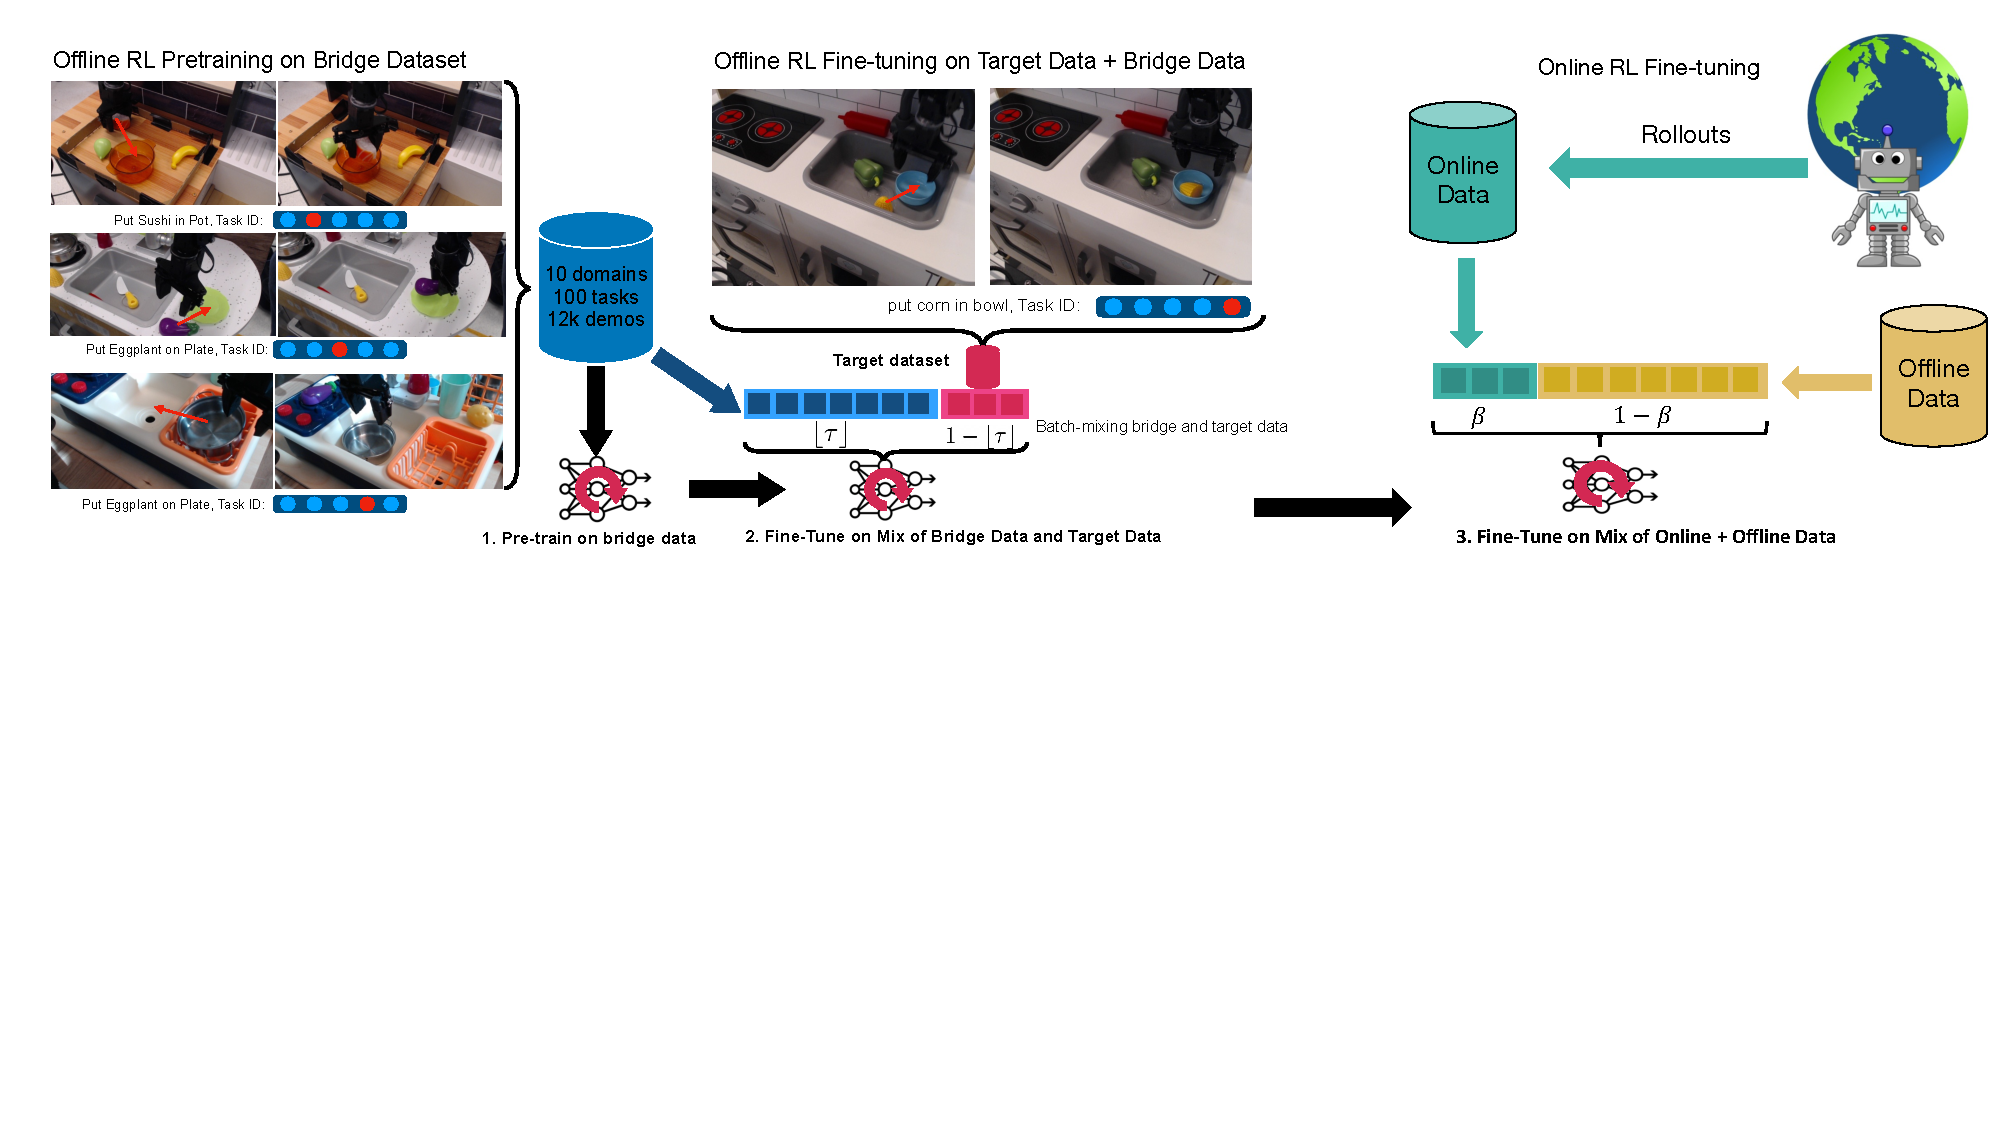
\includegraphics[width=0.9\linewidth]{system_overview.pdf}
  \vspace{-0.2cm}
  \captionof{figure}{ \label{fig:system_overview} \footnotesize \textbf{Overview of \methodname:} We first perform general offline pre-training on diverse multi-task robot data and subsequently fine-tune on one or several target tasks while mixing batches between the prior data and the target dataset using a batch mixing ratio of $\tau$. Additionally, a separate online fine-tuning phase can be done, where offline pre-training is done on a static dataset and an online replay buffer is collected using rollouts in the environment. The offline and online buffers are mixed per batch with a ratio of $\beta$.}
  \vspace{-0.35cm}
 }
\makeatother


\maketitle
\pagestyle{empty}

\begin{abstract}
Progress in deep learning highlights the tremendous potential of utilizing diverse robotic datasets for attaining effective generalization and makes it enticing to consider leveraging broad datasets for attaining robust generalization in robotic learning as well. However, in practice, we often want to learn a new skill in a new environment that is unlikely to be contained in the prior data. Therefore we ask: how can we leverage existing diverse offline datasets in combination with small amounts of task-specific data to solve new tasks, while still enjoying the generalization benefits of training on large amounts of data? In this paper, we demonstrate that end-to-end offline RL can be an effective approach for doing this, without the need for any representation learning or vision-based pre-training. We present pre-training for robots (PTR), a framework based on offline RL that attempts to effectively learn new tasks by combining pre-training on existing robotic datasets with rapid fine-tuning on a new task, with as few as 10 demonstrations. PTR utilizes an existing offline RL method, conservative Q-learning (CQL), but extends it to include several crucial design decisions that enable PTR to actually work and outperform a variety of prior methods. To our knowledge, PTR is the first RL method that succeeds at learning new tasks in a new domain on a real WidowX robot with as few as 10 task demonstrations, by effectively leveraging an existing dataset of diverse multi-task robot data collected in a variety of toy kitchens. We also demonstrate that PTR can enable effective autonomous fine-tuning and improvement in a handful of trials, without needing any demonstrations. An accompanying overview video can be found in the supplementary material and at this anonymous URL: \url{https://sites.google.com/view/ptr-rss}
\end{abstract}

\IEEEpeerreviewmaketitle


\section{Introduction}
\label{sec:intro}

% One of the primary drivers
% %\blfootnote{Correspondence to: Aviral Kumar (\texttt{aviralk@berkeley.edu})} 
% of the success of machine learning methods in open-world perception settings, such as computer vision~\cite{he2016resnet} and NLP~\cite{devlin2018bert}, has been the ability of high-capacity function approximators, such as deep neural networks, to learn generalizable models from large amounts of data. Reinforcement learning (RL) has proven comparatively difficult to scale to unstructured real-world settings because most RL algorithms require active data collection. As a result, RL algorithms can learn complex behaviors in simulation, where data collection is straightforward, 
% %~\cite{} \TODO{what's a good reference here?},
% %%SL.5.20: I think we could just omit any citation here, and cite all the RL stuff in the related work section. No need to needlessly spark a debate about whether Atari games, Go, or GTA driving require more or less generalization.
% but real-world performance is limited by the expense of active data collection. 
% %If we can develop effective off-policy RL methods, we would be able to train autonomous agents using large previously collected datasets. 
% In some domains, such as autonomous driving~\cite{yu2018bdd} and recommender systems~\citep{bennett2007netflix}, previously collected datasets are plentiful. Algorithms that can utilize such datasets effectively would not only make real-world RL more practical, but also would enable substantially better generalization by incorporating diverse prior experience.  

% aim in this paper is to devise off-policy RL algorithms that are stable and performant when trained entirely on off-policy experience, without any on-policy data collection.  
% Recent off-policy RL methods   (e.g.,~\citep{haarnoja2018sac,munos2016safe,kalashnikov18qtopt,impala2018}) have demonstrated sample-efficient performance on complex tasks in robotics~\cite{kalashnikov18qtopt} and simulated environments~\cite{mujoco}. 
% However, these methods can still fail to learn when presented with arbitrary off-policy data without the opportunity to collect more experience from the environment. This issue persists even when the off-policy data comes from effective expert policies, which in principle should address any exploration challenge~\citep{deBruin2015importance,fujimoto2018off,fu2019diagnosing}. This sensitivity to the training data distribution is a limitation of practical off-policy RL algorithms, and one would hope that an off-policy algorithm should be able to learn reasonable policies through training on static datasets before being deployed in the real world. %, without performance on the task decreasing as learning progresses. 

While state-of-the-art off-policy RL methods   (e.g.,~\citep{haarnoja2018sac,munos2016safe,kalashnikov18qtopt,impala2018}) have demonstrated sample-efficient performance on complex tasks in robotics~\cite{kalashnikov18qtopt} and in simulation~\cite{mujoco}, previously, we saw that these methods fail to learn when presented with arbitrary offline datasets. This issue persists even when the off-policy data comes from effective expert policies, which in principle should address any exploration challenge~\citep{deBruin2015importance,fujimoto2018off,fu2019diagnosing}. In this chapter, we aim to understand the root cause behind this inability and then develop off-policy, value-based RL methods that can learn from static, offline datasets. 

We show that a crucial challenge in applying value-based methods to off-policy scenarios arises in the bootstrapping process employed
when Q-functions are evaluated on out of \textit{out-of-distribution} action inputs for computing the backup when training from off-policy data. This may introduce errors in the Q-function and the algorithm is unable to collect new data in order to remedy those errors, making training unstable and divergent. We will first formalize and analyze the reasons for instability and poor performance when learning from off-policy data. Then, we will show that, through careful action selection, error propagation through the Q-function can be mitigated. We will then propose a principled algorithm called \emph{bootstrapping error accumulation reduction} (BEAR) to control bootstrapping error in practice, which uses the notion of \emph{support-set matching} to prevent error accumulation. Finally, through systematic experiments, we will show the effectiveness of our method on continuous-control MuJoCo Gym tasks, with a variety of off-policy datasets: generated by a random, suboptimal, or optimal policies. BEAR is consistently robust to the training dataset, matching or exceeding the state-of-the-art in all cases, whereas existing algorithms only perform well for specific datasets.


%Through systematic experiments, we demonstrate that this issue can lead to unstable, diverging, behavior (Sec.~\ref{sec:Problem Description}) during training.  %%SL.5.11: the above sentence doesn't actually say what we do -- what does it mean "we focus"? what are we doing?
%This includes state-of-the-art methods based on Q-learning~\citep{mnih2015humanlevel}, as well as actor-critic methods such as DDPG~\citep{lillicrap2015ddpg}, TD3~\cite{fujimoto18addressing}, and SAC~\citep{haarnoja2018sac}. This class of methods have been the focus of several theoretical analysis works that highlight the instabilities and sources of error that arise from the bootstrapping process employed by ADP methods~\citep{farahmand2010error}.
% In a standard supervised learning setup in machine learning, discrepancies between training performance and testing performance are often attributed to ``overfitting.'' However in reinforcement learning, agents suffer from substantial distribution shift, since updating the policy will change the distribution of states that the agent will experience. Simply obtaining more off-policy data from the same distribution is insufficient to guarantee stability in the learning process -- the design of stable off-policy algorithms must be observant of the fact that models will be evaluated at states with little data support over the course of training. In order to address problems related to learning from off-policy distributions, we analyze and address two major sources of error that arise from off-policy learning: bootstrapping error and evaluation error \textcolor{red}{TODO: make up better names for these}.
%Most of these ADP methods use bootstrapping to perform fixed point iteration with function approximators, which outputs an optimal policy at convergence. In this work, we analyse one major source of error that arises in these algorithms when learning with  static datasets -- which we call \textit{bootstrapping error}, and define next.
%%SL.5.11: We need to focus. The above paragraph casts the net a bit too broadly. If we focus on out-of-distribution actions, let's just motive that directly, instead of getting distracted with problems that are not the primary focus of our work. My recommendation would be to rewrite the above paragraph to focus exclusively on out-of-distribution action issues, and leave the rest for the discussion section.
%As Bellman error is typically minimized via supervised learning, the Q-values outside of training data. Moreover, function approximators used to model Q-functions in practice, have no guarantees whatsoever to produce reasonable values when queried with out-of-distribution inputs and can often generalize in unpredictable and undesired ways. These errors are hence, largely uncontrolled and these values can propagate to Q-values of neighboring states (which are then propagated further on subsequent iterations). 
%%SL.4.23: I think the above paragraph is reasonable, but it somewhat sweeps under the rug the critical observation: The issue here is that function approximators have no guarantees whatsoever to produce reasonable values when queried with out-of-distribution inputs. But this idea is missing in the above paragraph, and instead the issue is described in a way that is needlessly convoluted. Can we just state much more clearly that the problem is due to out-of-distribution inputs? This is good because it's not really an issue that prior work has thoroughly studied or addressed, due to lack of focus on function approximation. 
% The second source of error occurs from \textit{evaluating} the policy at states and actions not seen during training. When a policy is executed in an environment, it may inadvertently visit states that have not been experienced before. This can cause the policy to drift away from the training data during evaluation, causing compounding error over the course of an episode. This can happen, for instance, when training data exclusively comes from an expert policy, and during evaluation the policy visits a suboptimal state. Such issues have been extensively studied in imitation learning~\citep{ross2011dagger}, and we demonstrate that even in absence of bootstrapping error, this evaluation error can cause policies to be arbitrarily bad (Sec.~\ref{}).
%%SL.4.23: do we actually have a solution to this?
%%SL.4.23: The current introduction gets across the main idea, but it's a bit hard to parse and a bit technical. Can we more clearly draw out the common themes and state them out front? At a very fundamental level, both of these issues are issues due to out-of-distribution inputs, but they are also different from each other in perhaps a surprising way. Describing this simple fact early will make things look more coherent, and less like two disconnected and overly technical ideas.
%%SL.5.11: please address the above...
%%SL.5.11: also, the above discussion says nothing about how we address any of these problems
% Our primary contribution is 
%%SL.5.20: This seems like a pretty disappointing way to state the contribution. Can you more clearly state that the main contribution of our work is an analysis of bootstrapping error and a practical method for addressing it?
%%SL.4.23: another sentence about the results?
%%JF.4.25: I think we can just put a sentence on results in when we actually have them.

%%SL.5.11: We should rewrite the last paragraph to more directly describe what we do. Here is a potential phrasing:
% The main contribution in our paper is an analysis of several methods for stabilizing off-policy reinforcement learning. We first analyze the reasons for instability and poor performance when learning from off-policy data with approximate dynamic programming algorithms, using Q-learning and soft actor-critic~\cite{} in our analysis. We identify the out-of-distribution action problem and discuss its causes, and then propose three potential solutions. First, we show that actor-critic algorithms mitigate the issue both in theory and in practice, but only to a limited degree. Such methods remain susceptible to overtraining. Second, we show that a robust variant of importance sampling can greatly alleviate the out-of-distribution action problem, at the cost of severely conservative learning with poor final performance. Finally, we show that a combination of a pessimistic Q-value bound and a distributional support constraint mitigates the issue while maintaining good final performance. We analyze our method when learning from off-policy data with differing quality, ranging from random to near optimal, and on a range of discrete and continuous tasks. Our results show that mitigating the problem of out-of-distribution actions greatly improves the final performance and stability of off-policy RL.


%===============================================================================

\vspace{-0.2cm}
\section{Related Work}
\label{sec:related}
\vspace{-0.2cm}

Errors arising from inadequate sampling, distributional shift, and function approximation have been rigorously studied as ``error propagation'' in approximate dynamic programming (ADP)~\citep{bertsekas1996ndp,munos2003errorapi,farahmand2010error,bruno2015approximate}. These works often study how Bellman errors accumulate and propagate to nearby states via bootstrapping. In this chapter, we build upon tools from this analysis to show that performing Bellman backups on static datasets leads to error accumulation due to out-of-distribution values. Our approach is motivated as reducing the rate of propagation of error propagation between states.

BEAR constrains actor updates so that the actions remain in the support of the training dataset. Several works have explored similar ideas in the context of off-policy learning learning in online settings. \citet{kakade2002cpi} shows that large policy updates can be destructive, and propose a conservative policy iteration scheme which constrains actor updates to be small for provably convergent learning. \citet{grau-moya2018soft} use a learned prior over actions in the maximum entropy RL framework~\citep{levine2018rlasinference} and justify it as a regularizer based on mutual information. However, none of these methods use static datasets. Importance Sampling based distribution re-weighting~\cite{munos2016safe,gelada2019off,precup2001offpol,mahmood2015emphatic} has also been explored primarily in the context of off-policy policy evaluation.

Most closely related to our approach is batch-constrained Q-learning (BCQ)~\citep{fujimoto2018off} and SPIBB~\citep{laroche2019spibb}, which also discuss instability arising from previously unseen actions. \citet{fujimoto2018off} show convergence properties of an action-constrained Bellman backup operator in tabular, error-free settings. We prove stronger results under approximation errors and provide a bound on the \emph{suboptimality} of the solution. This is crucial as it drives the design choices for a practical algorithm. As a consequence, although we experimentally find that \citep{fujimoto2018off} outperforms standard Q-learning methods when the off-policy data is collected by an expert, BEAR outperforms \cite{fujimoto2018off} when the off-policy data is collected by a suboptimal policy, as is common in real-life applications. SPIBB~\citep{laroche2019spibb}, like BEAR, is an algorithm based on constraining the learned policy to the support of a behavior policy. However, the authors of SPIBB do not extend safe performance guarantees from the batch-constrained case to the relaxed support-constrained case, and do not study high-dimensional control tasks. 
% REM~\citep{agarwal19striving} is a concurrent work that uses a random convex combination of an ensemble of Q-networks to perform offline reinforcement learning from a static dataset consisting of interaction data generated while training a DQN agent.

	
%===============================================================================

\vspace{-0.2cm}
\section{Problem Statement and Definitions}
\vspace{-0.2cm}
% An RL algorithm aims to learn a policy in a Markov decision process (MDP), which is a tuple $\mathcal{M} = (\mathcal{S}, \mathcal{A}, \transitions, r, \mu_0, \gamma)$, where $\mathcal{S}, \mathcal{A}$ denote the state and action spaces, and
% $\transitions(\bs' | \bs, \mathbf{a})$, $r(\bs,\mathbf{a})$ represent the dynamics and reward function respectively. 
% $\mu_0(\bs)$ denotes the initial state distribution, and $\gamma \in (0,1)$ denotes the discount factor. The policy $\pi(\mathbf{a}|\bs)$ learned by RL agents must optimize the long-term cumulative reward, $\max_\policy J(\policy) := \E_{(\bs_t, \mathbf{a}_t) \sim \pi}[\sum_{t} \gamma^t r(\bs_t, \mathbf{a}_t)].$ 

\textbf{Problem statement.} Our goal is to learn general-purpose initializations from a broad, multi-task offline dataset and then fine-tune these initializations to specific downstream tasks. Following the notation from Chapter~\ref{chapter:cds_uds}, we denote the general-purpose offline dataset by $\mathcal{D}$, which is partitioned into $k$ chunks. Each chunk contains several transition typles for a given robotic task (e.g., picking and placing a given object) collected in a given domain (e.g., a particular kitchen). See \autoref{fig:system_overview} for an illustration. 
Formally, the dataset can be represented as $\mathcal{D} = \cup_{i=1}^k \left(i, \mathcal{D}_i \right)$, where we denote the set of training tasks concisely as $\mathcal{T}_{\text{train}} = [k]$. 
% Chunk $\mathcal{D}_i$ consists of data for a given task identifier $i$, and consists of a collection of transition tuples, $\mathcal{D}_i = \{(\bs^i_j, \mathbf{a}^i_j, r^i_j, \bs'^i_j)\}_{j=1}^n$ collected by a demonstrator on task $i$. 
% Each task has a different reward function.
Our goal is to utilize this multi-task dataset to help train a policy for one or multiple target tasks (denoted without loss of generality as task $\mathcal{T}_{\text{target}} = \{k+1, \cdots, n\}$). 

While the diverse prior dataset $\mathcal{D}$ does not contain any experience for the target tasks, in the offline fine-tuning setting, we are provided with a very small dataset of demonstrations $\mathcal{D}^* := \{\mathcal{D}_{k+1}^*, \mathcal{D}^*_{k+1}, \cdots, \mathcal{D}^*_n\}$ corresponding to each of the target tasks. In our experiments, we use only 10 to 15 demonstrations for each target task, making it impossible to learn the target task from this data alone, such that a method that effectively maximizes performance for the target tasks $\mathcal{T}_\text{target}$ must leverage the prior data $\mathcal{D}$. We also study the setting where we aim to quickly fine-tune the policy learned via offline pre-training and offline fine-tuning using limited amounts of autonomously collected data via online real-world interaction. More details about this are in Section~\ref{sec:experiments_online}.
 
%%AK: maybe problem statement and background should be different sections?
% \textbf{Background and preliminaries.} The Q-value of a given state-action tuple $Q^\pi(\bs, \mathbf{a})$ for a policy $\pi$ is the long-term discounted reward attained by executing action $\mathbf{a}$ at state $\bs$ and following policy $\pi$ thereafter. The Q-function satisfies the Bellman equation $Q^\pi(\bs, \mathbf{a}) = r(\bs, \mathbf{a}) + \gamma \mathbb{E}_{\bs', \mathbf{a}'}[Q^\pi(\bs', \mathbf{a}')]$. Typical model-free offline RL methods~\citep{fujimoto2018off,kumar2019stabilizing,kumar2020conservative} alternate between estimating the Q-function of a fixed policy $\pi$ using the offline dataset $\mathcal{D}$ and then improving the policy $\pi$ to maximize the learned Q-function. Our system, \ptrmethodname, utilizes one such model-free offline-RL method, conservative Q-learning (CQL)~\citep{kumar2020conservative}. We discuss how we adapt CQL for pre-training on diverse data followed by single-task fine-tuning in Section~\ref{sec:method}.

\textbf{Tasks and domains}. We use the Bridge Dataset~\cite{ebert2021bridge} as the source of our pre-training tasks, which we augment with a few additional tasks as discussed in Section~\ref{sec:result}. Our terminology for ``task'' and ``domain'' follows \citet{ebert2021bridge}: a task is a skill-object pair, such as ``put potato in pot'' and a domain corresponds to an environment, which in the case of the Bridge Dataset consists of different toy kitchens, potentially with different viewpoints and robot placements. We assume the new tasks and environments come from the same training distribution, but are not seen in the prior data.

% \begin{wrapfigure}{r}{7cm}
%   \vspace{-0.3cm}
%   \centering
%   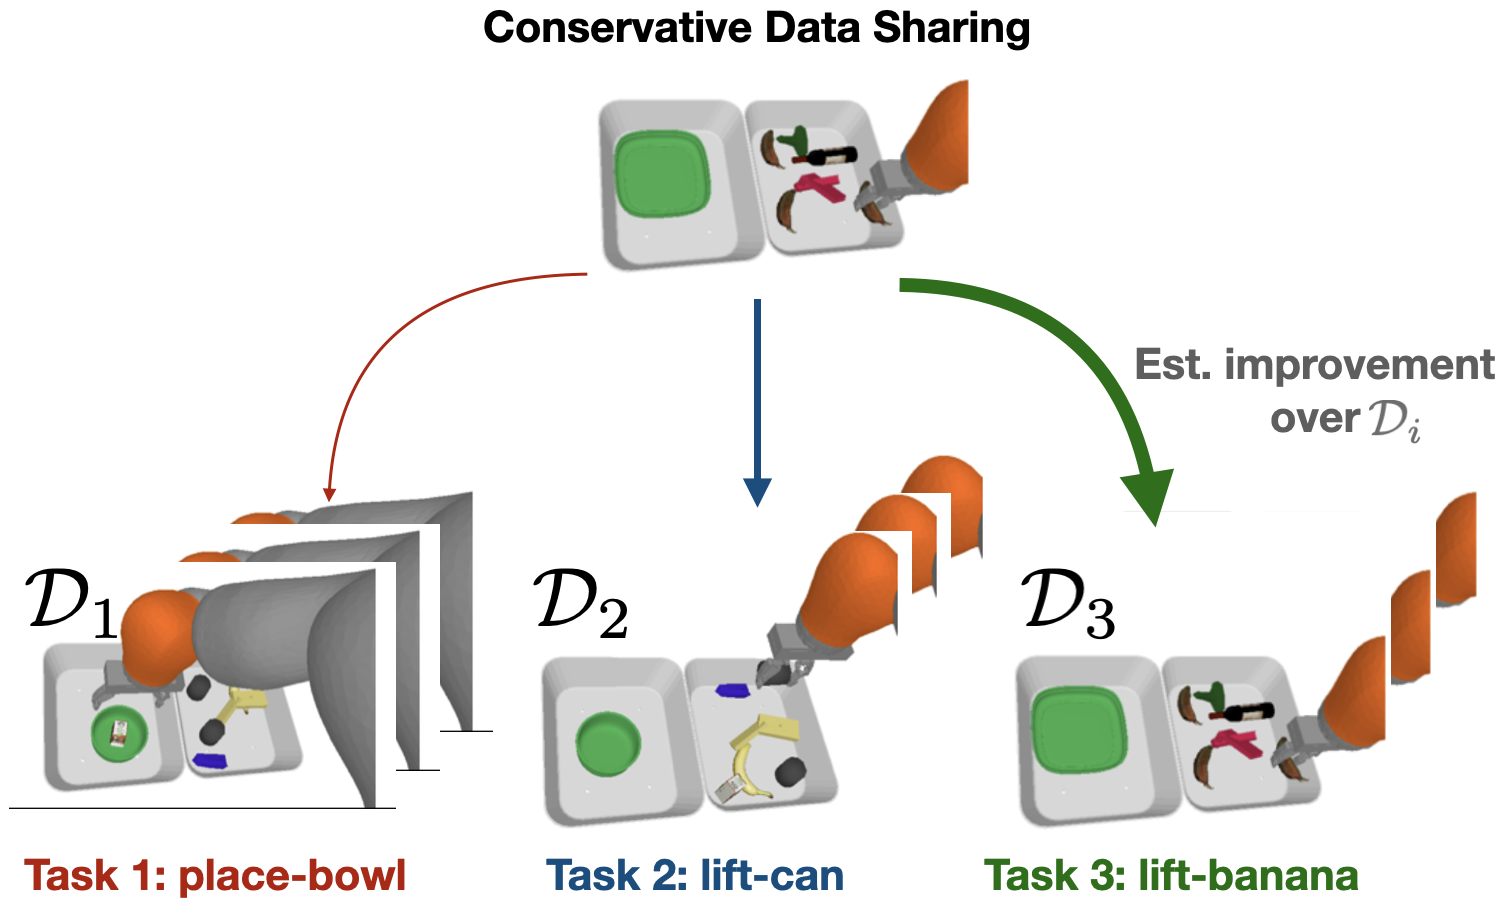
\includegraphics[width=0.45\textwidth]{chapters/cds/cds_teaser.png}
%   %%SL.7.31: consider making this a wrapfigure
%   \vspace{-0.2cm}
%   \caption{\footnotesize A visualization of \cdsmethodname, which routes a transition to
%   the offline dataset $\mathcal{D}_i$ for each task $i$ with a weight based on the estimated improvement over the behavior policy $\pi_\beta(\ba|\bs, i)$ of $\mathcal{D}_i$ after sharing the transition.}
%   \label{fig:teaser}
%   \vspace{-0.3cm}
% \end{wrapfigure}


\subsection{When Does Data Sharing Actually Help in Offline Multi-Task RL?}
\label{sec:analysis}
\vspace{-0.1cm}

Our goal is to leverage experience from all tasks to learn a policy for a particular task of interest. Perhaps the simplest approach to leveraging experience across tasks is to train the task policy on not just the data coming from that task, but also relabeled data from all other tasks~\citep{caruana1997multitask}. Is this na\"ive data sharing strategy sufficient for learning effective behaviors from multi-task offline data? In this section, we aim to answer this question via empirical analysis on a relatively simple domain, which will reveal interesting aspects of data sharing. We first describe the experimental setup and then discuss the results and possible explanations for the observed behavior. Using insights obtained from this analysis, we will then derive a simple and effective data sharing strategy in Section~\ref{sec:method}.

\textbf{Experimental analysis setup.} To assess the efficacy of data sharing, we experimentally analyze various multi-task RL scenarios created with the walker2d environment in Gym~\citep{brockman2016openai}. We construct different test scenarios on this environment that mimic practical situations, including settings where different amounts of  data of varied quality are available for different tasks~\citep{kalashnikov2021mt,xie2019improvisation,singh2020parrot}. In all these scenarios, the agent attempts three tasks: \texttt{run forward}, \texttt{run backward}, and \texttt{jump}, which we visualize in Figure~\ref{fig:env}. Following the problem statement in Section~\ref{sec:prelims}, these tasks share the same state-action space and transition dynamics, differing only in the reward function that the agent is trying to optimize. 
Different scenarios are generated with varying size offline datasets, each collected with policies that have different degrees of suboptimality. This might include, for each task, a single policy with mediocre or expert performance, or a mixture of policies given by the initial part of the replay buffer trained with online SAC~\citep{haarnoja2018soft}. We refer to these three types of offline datasets as medium, expert and medium-replay, respectively, following \citet{fu2020d4rl}.

We train a single-task policy $\pi_\mathrm{CQL}(\mathbf{a}|\bs, i)$ with CQL~\citep{kumar2020conservative} as the base offline RL method, along with two forms of data-sharing, as shown in Table~\ref{tab:analysis}: no sharing of data across tasks (\textbf{No Sharing}) and complete sharing of data with relabeling across all tasks (\textbf{Sharing All}). In addition, we also measure the divergence term in Equation~\ref{eqn:generic_multitask_offline_rl}, $D(\pi(\cdot|\cdot, i), \pi^\mathrm{eff}_\beta(\cdot|\cdot, i))$, for $\pi = \pi_\mathrm{CQL}(\mathbf{a}|\bs, i)$, averaged across tasks by using the
Kullback-Liebler divergence. This value quantifies the average divergence between the single-task optimal policy and the relabeled behavior policy averaged across tasks.  

\begin{table*}[t]
\centering
\scriptsize
\def\arraystretch{0.9}
\setlength{\tabcolsep}{0.42em}
\resizebox{0.95\textwidth}{!}{\begin{tabular}{cc|cc|cc}
  \toprule
 \multicolumn{1}{c}{\multirow{1.5}[2]{*}{Dataset types / Tasks}} & \multicolumn{1}{c}{\multirow{1.5}[2]{*}{Dataset Size}}\vline &
 \multicolumn{2}{c}{Avg Return}\vline & \multicolumn{2}{c}{$D_\text{KL}(\pi, \pi_\beta)$}\\
 & \multicolumn{1}{c}{}\vline & \multicolumn{1}{c}{\textbf{No Sharing}}  & \multicolumn{1}{c}{\textbf{Sharing All}}\vline  & \multicolumn{1}{c}{\textbf{No Sharing}}  & \multicolumn{1}{c}{\textbf{Sharing All}} \\
\midrule
  medium-replay / \texttt{run forward} & 109900 & \textbf{998.9} & 966.2 & \textbf{3.70} & 10.39\\
  medium-replay / \texttt{run backward} & 109980 & \textbf{1298.6} & 1147.5 & \textbf{4.55} & 12.70\\
  medium-replay / \texttt{jump} & 109511 & \textbf{1603.1} & 1224.7 & \textbf{3.57} & 15.89\\
  \rowcolor{Gray}
  \textbf{average task performance} & N/A & \textbf{1300.2} & 1112.8 & \textbf{3.94}  & 12.99\\
  \midrule
  medium / \texttt{run forward} & 27646 & 297.4  & \textbf{848.7} &\textbf{6.53} & 11.78\\
  medium / \texttt{run backward} & 31298 & 207.5 & \textbf{600.4}& \textbf{4.44} & 10.13\\
  medium / \texttt{jump} & 100000 & 351.1 & \textbf{776.1}& \textbf{5.57} & 21.27\\
%   \hline
\rowcolor{Gray}
  \textbf{average task performance} & N/A & 285.3 & \textbf{747.7} & \textbf{5.51} & 14.39 \\
  \midrule
  medium-replay / \texttt{run forward} & 109900 & 590.1 & \textbf{701.4}& \textbf{1.49} & 7.76\\
  medium / \texttt{run backward} & 31298 & 614.7 & \textbf{756.7}& \textbf{1.91} & 12.2\\
  \rowcolor{yellow}
  expert / \texttt{jump} & 5000 & \textbf{1575.2} & 885.1 & \textbf{3.12} & 27.5\\
%   \hline
\rowcolor{Gray}
  \textbf{average task performance} & N/A & \textbf{926.6} & 781 & \textbf{2.17}  & 15.82 \\
    \bottomrule
\end{tabular}}
    \vspace{-0.1cm}
         \caption{\footnotesize We analyze how sharing data across all tasks (\textbf{Sharing All}) compares to \textbf{No Sharing} in the multi-task walker2d environment with three tasks: run forward, run backward, and jump. We provide three scenarios with different styles of per-task offline datasets in the leftmost column. The second column shows the number of transitions in each dataset. We report the per-task average return, the KL divergence between the single-task optimal policy $\pi$ and the behavior policy $\behavior$ after the data sharing scheme, as well as averages across tasks. \textbf{Sharing All} generally helps training while increasing the KL divergence. However, on the row highlighted in yellow, \textbf{Sharing All} yields a particularly large KL divergence between the single-task $\pi$ and $\behavior$ and degrades the performance, suggesting sharing data for all tasks is brittle.
     \label{tab:analysis}
     \vspace{-0.2cm}
     }
\end{table*}

\textbf{Analysis of results in Table~\ref{tab:analysis}.} To begin, note that even na\"ively sharing data is  better than not sharing any data at all on \textbf{5/9} tasks considered
(compare the performance across \textbf{No Sharing} and \textbf{Sharing All} in Table~\ref{tab:analysis}). However, a closer look at Table~\ref{tab:analysis} suggests that data-sharing can significantly degrade performance on certain tasks, especially in scenarios where the amount of data available for the original task is limited, and where the distribution of this data is narrow.
For example, when using expert data for jumping in conjunction with more than 25 times as much lower-quality (mediocre \& random) data for running forward and backward, we find that the agent performs poorly on the jumping task despite access to near-optimal jumping data.

~

\niparagraph{\emph{Why does na\"ive data sharing degrade performance on certain tasks despite near-optimal behavior for these tasks in the original task dataset?}} We argue that the primary reason that na\"{i}ve data sharing can actually hurt performance in such cases is because it exacerbates the distributional shift issues that afflict offline RL. Many offline RL methods combat distribution shift by implicitly or explicitly constraining the learned policy to stay close to the training data. Then, when the training data is changed by adding relabeled data from another task, the constraint causes the learned policy to change as well. When the added data is of low quality for that task, it will correspondingly lead to a lower quality learned policy for that task, unless the constraint is somehow modified. This effect is evident from the higher divergence values between the learned policy without any data-sharing and the effective behavior policy for that task \emph{after} relabeling (e.g., expert+\texttt{jump}) in Table~\ref{tab:analysis}. Although these results are only for CQL, we expect that any offline RL method would, insofar as it combats distributional shift by staying close to the data, would exhibit a similar problem. 


\niparagraph{\textbf{To mathematically quantify}} the effects of data-sharing in multi-task offline RL, we appeal to safe policy improvement bounds~\citep{laroche2019safe,kumar2020conservative,yu2021combo} and discuss cases where data-sharing between tasks $i$ and $j$ can degrade the amount of worst-case guaranteed improvement over the behavior policy. Prior work~\citep{kumar2020conservative} has shown that the generic offline RL algorithm in Equation~\ref{eqn:generic_offline_rl} enjoys the following guarantees of policy improvement on the actual MDP, beyond the behavior policy: 
\begin{align}
\label{eqn:spi}
    J(\pi^*) &\geq J(\pi_\beta) - \mathcal{O}(1/ (1 - \gamma)^2) \mathbb{E}_{\bs, \mathbf{a} \sim d^{\pi}} \left[\sqrt{\frac{D(\pi(\cdot|\bs), \pi_\beta(\cdot|\bs))}{|\mathcal{D}(\bs)|}}\right] + \alpha/(1 - \gamma) D(\pi, \pi_\beta).
\end{align}
We will use Equation~\ref{eqn:spi} to understand the scenarios where data sharing can hurt. When data sharing modifies $\mathcal{D} = \mathcal{D}_i$ to $\mathcal{D} = \mathcal{D}^\mathrm{eff}_i$, which includes $\mathcal{D}_i$ as a subset, it effectively aims at reducing the magnitude of the second term (i.e., sampling error) by increasing the denominator. This can be highly effective if the state distribution of the learned policy $\pi^*$ and the dataset $\mathcal{D}$ overlap. However, an increase in the divergence $D(\pi(\cdot|\bs), \pi^\beta(\cdot|\bs))$ as a consequence of relabeling implies a potential increase in the sampling error, unless the increased value of $|\mathcal{D}^\mathrm{eff}(\bs)|$ compensates for this. Additionally, the bound also depends on the quality of the behavior data added after relabeling: if the resulting behavior policy $\pi^\mathrm{eff}_\beta$ is more suboptimal compared to $\pi_\beta$, i.e., $J(\pi^\mathrm{eff}_\beta) < J(\pi_\beta)$, then the guaranteed amount of improvement also reduces.

% \begin{proposition}[Na\"ive data-sharing can hurt policy performance.] Assume that the the multi-task MDP consists of discrete states $\mathcal{S}$ and actions $\mathcal{A}$. Consider the scenario where data from task $\mathcal{T}_j$, $\mathcal{D}(\mathcal{T}_j)$, is relabelled to task $\mathcal{T}_i$ and let $\mathcal{D}_\mathrm{eff}(\mathcal{T}_i) = \mathcal{D}(\mathcal{T}_j \rightarrow \mathcal{T}_i) \cup \mathcal{D}(\mathcal{T}_i)$. For any dataset, let $|\mathcal{D}(\bs)|$ be the frequency of a state $\bs$ in $\mathcal{D}$, $\pi^*(\mathbf{a}|\bs, \mathcal{T}_i)$ denote the optimal solution to Equation~\ref{eqn:generic_multitask_offline_rl} without any data sharing and let $\pi^*_\mathrm{eff}(\mathbf{a}|\bs)$ be the optimal solution of Equation~\ref{eqn:generic_multitask_offline_rl} with data sharing. Let $\pi^\mathrm{eff}_\beta(\mathbf{a}|\bs, \mathcal{T}_i)$ denote the effective behavior policy for $\mathcal{D}_\mathrm{eff}(\mathcal{T}_i)$. Then, sharing data from task $\mathcal{T}_j$ to task $\mathcal{T}_i$ may not improve the resulting policy performance on task $\mathcal{T}_i$, i.e., $J(\pi^*, \mathcal{T}_i) \geq J(\pi^*_\mathrm{eff}, \mathcal{T}_i) + \zeta$, in the worst-case where:
% \begin{equation*}
%     \zeta \geq  C \mathbb{E}_{\bs, \mathbf{a} \sim d^{\pi^*}} \left[ \sqrt{\frac{D(\pi(\cdot|\bs), \pi^\mathrm{eff}_\beta(\cdot|\bs))}{{|\mathcal{D}_\mathrm{eff}(\mathcal{T}_i)(\bs)|}}} \right] - C \mathbb{E}_{\bs, \mathbf{a} \sim d^{\pi^*}} \left[ \sqrt{\frac{D(\pi(\cdot|\bs), \pi_\beta(\cdot|\bs))}{{|\mathcal{D}(\mathcal{T}_i)(\bs)|}}} \right] + J_{\mathcal{T}_i}(\pi_\beta) - J_{\mathcal{T}_i}(\pi_\beta^\mathrm{eff}) 
% \end{equation*}
% where $C$ is a universal constant depending on the MDP, $d^{\pi^*}$ denotes the state-action marginal of policy $\pi^*$ on the MDP and $\varepsilon > 0$.
% \label{prop:data_sharing}
% \end{proposition}
% While the inequality in Proposition~\ref{prop:data_sharing} is only a bound on performance, it still reveals some tradeoffs associated with data sharing: when data sharing induces distributional shift, such that the value of $D(\pi, \pi^\mathrm{eff}_\beta)$ increases compared to $D(\pi, \pi_\beta)$, without increasing visitation frequencies of states under the learned single-task policy, such that $|\mathcal{D}_\mathrm{eff}(\mathcal{T}_i)(\bs)|$ does not increase enough
% beyond $|\mathcal{D}(\mathcal{T}_i)(\bs)|$ to compensate for the increase in $D(\pi, \pi^\mathrm{eff}_\beta)$, poor performance might be obtained.
% %%SL.5.23: what about the proposition indicates that poor performance might be obtained? can we make this part of the statement more precise?
% The performance decrease is exacerbated when the data being shared is of low quality, i.e., $J(\pi_\beta^\mathrm{eff}) \leq J(\pi_\beta)$. 
% %%AK: maybe we should also have a figure illustrating the spectrum of data-sharing: there is an optimistic end, share everything, a conservative end, share nothing and the more conservative side of the spectrum where our method lies? This is kinda like what I had drawn earlier on the jamboard notes when we discussed a few months back.

% Two considerations: (1) task alignment (2) different dataset types, which can hurt optimziation. Summarioze the main "rules", phenomenon by this this happens. Consequences -- conservative or you become optimistic, etc
% To conclude, we observe that while na\"ive data sharing can generally help improve performance in multi-task offline RL, but that the behavior policy coupled with the amount of data observed can have a significant impact on the performance of na\"ive data sharing. This may prevent existing algorithms from leveraging large pre-existing datasets of potentially useful, but not directly-relevant behaviors to improve performance, thereby hindering generalization. In the next section, we present our method, \cdsmethodname,  that addresses this issue and is derived via a principled optimization problem that aims to maximize per-task performance.

\textbf{To conclude,} our analysis reveals that while data sharing is often helpful in multi-task offline RL, it can lead to substantially poor performance on certain tasks as a result of exacerbated distributional shift between the optimal policy and the effective behavior policy induced after sharing data. 
% Thus, in order to obtain effective policies for all tasks in this setting, we propose to share data \emph{conservatively},
% with precaution taken to not exacerbate distributional shift via relabeling. This forms the basis of our data-sharing scheme, \cdsmethodname, which we will discuss next.

% \vspace{-5pt}
% \section{Regimes of Data Sharing in Multi-Task Offline RL}
% \label{sec:different_regimes}
% The analysis in Section~\ref{sec:analysis} shows that na\"ive data sharing may be highly sub-optimal in some cases, and although it often does improve over no data sharing at all in practice, it can also lead to exceedingly poor performance. On the other hand, no data sharing can also lead to poor performance since it is overly conservative, and does not share any experience at all. In this section, we aim to understand the spectrum in between no data sharing and complete data sharing, aiming to understand the kinds of data sharing schemes that provide a balanced tradeoff between no data sharing and full data sharing. We will then use the insights gathered from this section to derive a complete method in Section~\ref{sec:method}.

% Since full data sharing exacerbates distributional shift, a simple data sharing strategy could be to share data only when distributional shift is reduced. That is, more formally, for any given transition $(\bs, \mathbf{a}, r, \bs')$, this scheme would compare $D(\pi, \pi_\beta)(\bs)$ and $D(\pi, \pi^{\text{eff}}_\beta)(\bs)$ and utilize the transition for training only when $D(\pi, \pi_\beta)(\bs) \geq D(\pi, \pi_\beta^\text{eff})(\bs)$. We refer to this scheme as X. 

% While X provably alleviates the concerns of increasing distribution shift as a result of data sharing, it is overly conservative in practice. A distinct, more optimistic scheme for data sharing is to share a use a transition $(\bs, \mathbf{a}, r, \bs')$ for training only if the resulting data improves upon the learned policy performance.   

\vspace{-5pt}
\subsection{\cdsmethodname: Reducing Distributional Shift in Multi-Task Data Sharing}
\label{sec:method}
\vspace{-5pt}
The analysis in Section~\ref{sec:analysis} shows that na\"ive data sharing may be highly sub-optimal in some cases, and although it often does improve over no data sharing at all in practice, it can also lead to exceedingly poor performance. Can we devise a conservative approach that shares data intelligently to not exacerbate distributional shift as a result of relabeling?
%%CF.8.1: This question above is super long, and starts to get incomprehensible towards the end. Can you shorten or split it up? And, what's the difference between the benefits of sharing data and the benefits of sharing data of high quality?? I think that my suggested edit should fix this.
%%AK: addressed, just kept the first part of this since the story of quality and sampling error comes in after 5.1

\subsubsection{A First Attempt at Designing a Data Sharing Strategy}
A straightforward data sharing strategy is to utilize a transition for training only if it reduces the distributional shift.
%%SL.8.1: The above sentence comes across as a bit obtuse -- of course doing X only if it reduces distributional shift will, by definition, not increase distributional shift -- can you rephrase?
%%CF.8.1: +1. Maybe "A starightforward data sharing strategy is to utilize a transition for training only if it reduces the distribution shift."
%%AK: done
Formally, this means that for a given transition $(\bs, \mathbf{a}, r_j(\bs, \mathbf{a}), \bs') \in \mathcal{D}_j$ sampled from the dataset $\mathcal{D}_j$, such a scheme would prescribe using it for training task $i$ (i.e., $(\bs, \mathbf{a}, r_i(\bs, \mathbf{a}), \bs') \in \mathcal{D}^\mathrm{eff}_i$) only if: 
%%CF.8.1: can you simplify the structure of the above sentence? it is a lot to take in and will probably require the reader to read it twice in its current form.
%%AK: slightly reogranized. Is it still too hard to read?
\begin{tcolorbox}[colback=blue!6!white,colframe=black,boxsep=0pt,top=-3pt,bottom=2pt]
\begin{equation}
\label{eqn:pessimistically_conservative}
    \text{\textbf{CDS (basic)}:}~~~~~~~\Delta^\pi(\bs, \mathbf{a}) := D(\pi(\cdot|\cdot, i), \pi_\beta(\cdot|\cdot, i))(\bs) - D(\pi(\cdot|\cdot, i), \pi_\beta^{\text{eff}}(\cdot|\cdot, i))(\bs) \geq 0. 
\end{equation}
\end{tcolorbox}
%%AK: the above equation is not technically correct, since there is no a on the right side of \Delta^\pi(s, a), need to fix this.
The scheme presented in Equation~\ref{eqn:pessimistically_conservative} would guarantee that distributional shift (i.e., second term in Equation~\ref{eqn:generic_multitask_offline_rl}) is reduced.
%%CF.8.1: i.e. that distribution shift is reduced.
%%AK: done
Moreover, since sharing data can only increase the size of the dataset and not reduce it, this scheme is guaranteed to not increase the sampling error term in Equation~\ref{eqn:spi}. We refer to this scheme as the basic variant of conservative data sharing (\textbf{CDS (basic)}).
%%CF.8.1: hmm, I wouldn't recommend forward referencing equations like this.
%%AK: this was an error in the equatino refercing, this question appears before.

While this scheme can prevent the negative effects of increased distributional shift, this scheme is quite pessimistic. Even in our experiments, we find that this variant of CDS does not improve performance by a large margin.
%%TY.8.2: did our experiments show this? Maybe we should rephrase to "we find that this variant of CDS performs underwhelmingly, achieving worse results compared to the naively data sharing and no data sharing approaches".
%%AK: done
Additionally, as observed in Table~\ref{tab:analysis} (medium-medium-medium data composition) and discussed in Section~\ref{sec:analysis}, data sharing can often be useful despite an increased distributional shift (note the higher values of $D_\mathrm{KL}(\pi, \pi_\beta)$ in Table~\ref{tab:analysis}) likely because it reduces sampling error and potentially utilizes data of higher quality for training. \textbf{CDS (basic)} described above does not take into account these factors. Formally, the effect of the first term in Equation~\ref{eqn:generic_multitask_offline_rl}, $J_{\mathcal{D}^\text{eff}}(\pi)$ (the policy return in the empirical MDP generated by the dataset) and a larger increase in $|\mathcal{D}^\mathrm{eff}(\bs)|$ at the cost of somewhat increased value of $D(\pi(\cdot|\bs), \pi_\beta(\cdot|\bs)$ are not taken into account. Thus we ask: can we instead design a more complete version of CDS that effectively balances the tradeoff by incorporating all the discussed factors (distributional shift, sampling error, data quality)?  
% This term is guaranteed to increase with the scheme in Equation~\ref{eqn:pessimistically_conservative} in practice, since this scheme only utilizes \emph{additional} data corresponding to other tasks for training which would not reduce the performance of the policy compared to no sharing. Combined with the reduced value of the second term, this implies that this scheme increases the objective in Equation~\ref{eqn:generic_multitask_offline_rl}. 

%%SL.8.1: In the interest of space, I think this paragraph can largely be cut, since the end of the previous paragraph already motivates the need for a less conservative method. You could cut this and replace it with a sentence or two at the beginning of the next section.
%%CF.8.1: +1
% \textbf{Is p-CDS sufficient for effective multi-task offline RL?} While p-CDS guarantees that the shared data will not exacerbate distributional shift, which is quite useful in cases such as the walker2d expert scenario analyzed in Section~\ref{sec:analysis}, this scheme can be overly pessimistic. As we also find in our experiments in Section~\ref{sec:exp}, p-CDS often chooses to not share any data in scenarios where it is impossible to meet the strong requirement of reduced distributional shift. On the other side, in a number of scenarios, data sharing improves performance because more training data stabilizes training and reduces sampling error and improves the quality of the data in the dataset, albeit at the cost of slightly increased distributional shift. This raises the question: Can we devise a conservative data sharing scheme that instead \emph{optimistically} shares data, by effectively balancing the improvement due to reduced sampling error and increased data quality, and a deterioration due to increased distributional shift? Such an optimistic scheme would not only reduce the second term in Equation~\ref{eqn:generic_multitask_offline_rl}, but would also share data if the gain in the first term $J_{\mathcal{D}^\text{eff}}(\pi)$ outweighs a slight increase in distributional shift. This is the key idea behind \textbf{optimistically conservative data sharing (o-CDS)} that we discuss next.

\subsubsection{The Complete Version of Conservative Data Sharing (CDS)}
\label{sec:complete_cds}
\begin{wrapfigure}{r}{0.5\textwidth}
\centering
\vspace{-0.7cm}
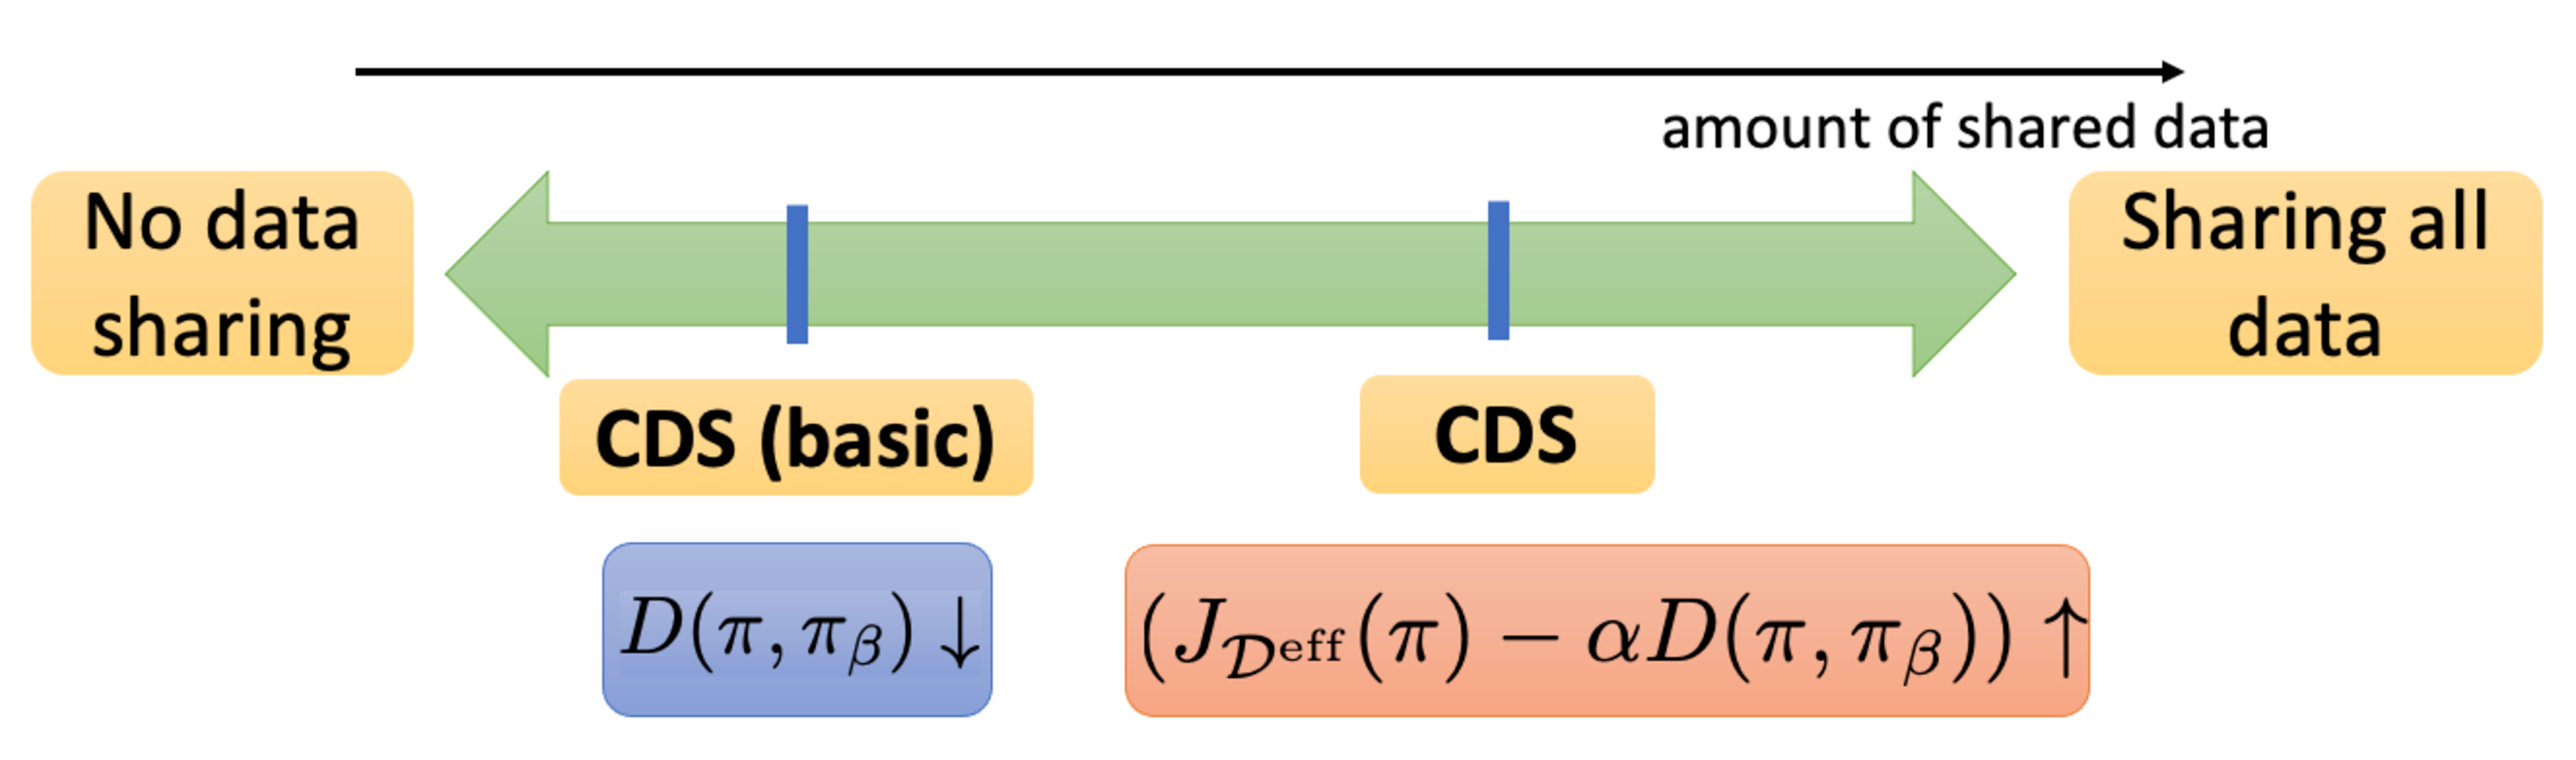
\includegraphics[width=0.99\linewidth]{chapters/cds/cds_variants.pdf}
%%CF.8.1: I think this is a nice figure. My only comment is that it isn't clear what "naive data sharing" means without having read parts of the main text. (and you should expect readers to skim figures without reading all of the text. I would change it to something like "Sharing all data" instead.
\vspace{-0.6cm}
\caption{\label{fig:cds_variants_main} \footnotesize A schematic comparing \textbf{CDS} and \textbf{CDS (basic)} data sharing schemes relative to no sharing (left extreme) and full data sharing (right extreme). While p-CDS only shares data when distributional shift is strictly reduced, o-CDS is more optimistic and shares data when the objective in Equation~\ref{eqn:generic_multitask_offline_rl} is larger. Typically, we would expect that CDS shares more transitions than CDS (basic).}
\vspace{-0.6cm}
\end{wrapfigure}
Next, we present the complete version of our method. The complete version of CDS, which we will refer to as \textbf{CDS}, for notational brevity is derived from the following perspective: we note that a data sharing scheme can be viewed as altering the dataset $\mathcal{D}^\mathrm{eff}_i$, and hence the effective behavior policy, $\pi^\mathrm{eff}_\beta(\mathbf{a}|\bs, i)$.
Thus, we can directly \emph{optimize} the objective in Equation~\ref{eqn:generic_multitask_offline_rl} with respect to $\pi^\mathrm{eff}_\beta$,
in addition to $\pi$, where $\pi^\mathrm{eff}_\beta$ belongs to the set of all possible effective behavior policies that can be obtained via any form of data sharing. Note that unlike CDS (basic), this approach would not rely on only indirectly controlling the objective in Equation~\ref{eqn:generic_multitask_offline_rl} by controlling distributional shift, but would aim to directly optimize the objective in Equation~\ref{eqn:generic_multitask_offline_rl}.  We formalize this optimization below in Equation~\ref{eqn:optimize_behavior}:
\begin{align}
\label{eqn:optimize_behavior}
    % &(\pi^*(\cdot|\cdot, i), \pi^\mathrm{eff}_\beta(\cdot|\cdot, i))\nonumber\\
    \arg \max_{\pi} \textcolor{red}{\max_{\pi^\mathrm{eff}_\beta \in \Pi_{\mathrm{relabel}}}}~~~ \left[J_{\mathcal{D}^\mathrm{eff}_i}(\pi) - \alpha D(\pi, \pi^\mathrm{eff}_\beta; i)\right],
\end{align}
where $\Pi_{\mathrm{relabel}}$ denotes the set of all possible behavior policies that can be obtained via relabeling. The next result characterizes safe policy improvement for Equation~\ref{eqn:optimize_behavior} and discusses how it leads to improvement over the behavior policy and also produces an effective practical method.

\begin{tcolorbox}[colback=blue!6!white,colframe=black,boxsep=0pt,top=-3pt,bottom=2pt]
\vspace{2mm}
\begin{proposition}[Characterizing safe-policy improvement for CDS.] 
\label{prop:spi_thm}
Let $\pi^*(\mathbf{a}|\bs)$ be the policy obtained from Equation~\ref{eqn:optimize_behavior}, and let $\pi_\beta(\mathbf{a}|\bs)$ be the behavior policy for $\mathcal{D}_i$. Then, w.h.p. $\geq 1 - \delta$, $\pi^*$ is a $\zeta$-safe policy improvement over $\pi_\beta$, i.e., $J(\pi^*) \geq J(\pi_\beta) - \zeta$, where $\zeta$ is given by:
\begin{align*}
\small{
    \!\!\zeta = \mathcal{O}\left(\frac{1}{(1 - \gamma)^2}\right)  \mathbb{E}_{\bs \sim d^{\pi^*}_{\mathcal{D}^\mathrm{eff}_i}}\left[\sqrt{\frac{D_{\text{CQL}}(\pi^*, \pi_\beta^*)(\bs) + 1}{|\mathcal{D}^\mathrm{eff}_i(\bs)|}} \right]
    -  \left[\alpha D(\pi^*, \pi_\beta^*) + \underbrace{J(\pi^*_\beta) - J(\pi_\beta)}_{\text{(a)}} \right],}
\end{align*}
\!\!where $\mathcal{D}^\mathrm{eff}_i \sim d^{\pi_\beta^*}(\bs)$ and $\pi^*_\beta(\mathbf{a}|\bs)$ denotes the policy $\pi \in \Pi_{\text{relabel}}$ that maximizes Equation~\ref{eqn:optimize_behavior}. 
\end{proposition}
\end{tcolorbox}
%%CF.8.1: I might consider putting this theoretical result back to the appendix. Right now, the main method doesn't come until the bottom of page 7, and the practical implementation doesn't come until page 8. Given that you can only really expect the reader to read ~9 pages, I think that the core info about the method is more important than this theoretical result.

A proof and analysis of this proposition is provided in Appendix~\ref{app:proofs}, where we note that the bound in Proposition~\ref{prop:spi_thm} is stronger than both no data sharing as well as na\"ive data sharing. We show in Appendix~\ref{app:proofs} that optimizing Equation~\ref{eqn:optimize_behavior} reduces the numerator $D_\mathrm{CQL}(\pi^*, \pi_\beta^*)$ term while also increasing $|\mathcal{D}^\mathrm{eff}_i(\bs)|$, thus reducing the amount of sampling error. In addition, Lemma~\ref{lemma:a_gt_0} shows that the improvement term $(a)$ is guaranteed to be positive if a large enough $\alpha$ is chosen in Equation~\ref{eqn:optimize_behavior}. Combining these, we find data sharing using Equation~\ref{eqn:optimize_behavior} improves over both complete data sharing (which may increase $D_\mathrm{CQL}(\pi, \pi_\beta)$) and no data sharing (which does not increase $|\mathcal{D}^\mathrm{eff}_i(\bs)|$). A schematic comparing the two variants of CDS and na\"ive and no data sharing schemes is shown in Figure~\ref{fig:cds_variants_main}.

~

\niparagraph{\textbf{Optimizing Equation~\ref{eqn:optimize_behavior} tractably.}} 
The next step is to effectively convert Equation~\ref{eqn:optimize_behavior} into a simple condition for data sharing in  multi-task offline RL. While directly solving Equation~\ref{eqn:optimize_behavior} is intractable in practice, since both the terms depend on $\pi^\mathrm{eff}_\beta(\mathbf{a}|\bs)$ (since the first term $J_{\mathcal{D}^\mathrm{eff}}(\pi)$ depends on the empirical MDP induced by the effective behavior policy and the amount of sampling error), we need to instead  solve Equation~\ref{eqn:optimize_behavior} approximately. Fortunately, we can optimize a \textit{lower-bound approximation} to Equation~\ref{eqn:optimize_behavior} that uses the dataset state distribution for the policy update in Equation~\ref{eqn:optimize_behavior} similar to modern actor-critic methods~\citep{degris2012off,lillicrap2015continuous,fujimoto2018addressing,haarnoja2018soft,kumar2020conservative} which only introduces an additional $D(\pi, \pi_\beta)$ term in the objective. This objective is given by: $\mathbb{E}_{\bs \sim \mathcal{D}^{\mathrm{eff}}_i}[\mathbb{E}_\pi[Q(\bs, \mathbf{a}, i)] - \alpha' D(\pi(\cdot|\bs,i), \pi_\beta^\mathrm{eff}(\cdot|\bs,i))]$, which is equal to the expected ``conservative Q-value'' $\hat{Q}^\pi(\bs, \mathbf{a}, i)$ on dataset states, policy actions and task $i$. Optimizing this objective via a co-ordinate descent on $\pi$ and $\pi^\mathrm{eff}_\beta$ dictates that $\pi$ be updated using a standard update of maximizing the conservative Q-function, $\hat{Q}^\pi$ (equal to the difference of the Q-function and $D(\pi, \pi^{\mathrm{eff}}_\beta; i)$).
Moreover, $\pi^{\mathrm{eff}}_\beta$ should also be updated towards maximizing the same expectation, $\mathbb{E}_{\bs, \mathbf{a} \sim \mathcal{D}^\mathrm{eff}_i}[\hat{Q}^\pi(\bs, \mathbf{a}, i)] := \mathbb{E}_{\bs, \mathbf{a} \sim \mathcal{D}^\mathrm{eff}_i}[Q(\bs, \mathbf{a}, i)] - \alpha D(\pi, \pi_\beta^\mathrm{eff}; i)$. This implies that when updating the behavior policy, we should prefer state-action pairs that maximize the conservative Q-function.
% Additionally $\pi^{\mathrm{eff}}_\beta$ should be updated towards minimizing the distribution shift $\mathbb{E}_{\bs, \mathbf{a} \sim \mathcal{D}^\mathrm{eff}_i}[ D(\pi, \pi_\beta^\mathrm{eff}; i)]$, i.e. learning a new behavior policy of task $i$ with minimal distribution shift after relabeling. In the case where $D(\pi, \pi_\beta^\mathrm{eff}; i) = D_\text{CQL}(\pi, \pi_\beta^\mathrm{eff}; i)$, we have the following objective for updating $\pi_\beta$: $\min_{\pi_\beta}\mathbb{E}_{\bs, \mathbf{a} \sim \mathcal{D}^\mathrm{eff}_i}[\hat{Q}^\pi(\bs,\mathbf{a}, i)]$
% \begin{align}
%     J_{\mathcal{D}^\mathrm{eff}_i}(\pi) - \alpha D(\pi, \pi^\mathrm{eff}_\beta; i) &:= \mathbb{E}_{\bs, \mathbf{a} \sim d^\pi_{\mathrm{eff}}}\left[Q(\bs, \mathbf{a}) - \alpha D(\pi, \pi_\right] 
% \end{align}

~

\niparagraph{\textbf{{Deriving the data sharing strategy for CDS.}}}
%%SL.8.1: not clear what the word "condition" means
%%CF.8.1: +1. What condition are you deriving?
%%AK: fixed
Utilizing the insights for optimizing Equation~\ref{eqn:optimize_behavior} tractably, we now present the effective data sharing rule prescribed by CDS. For any given task $i$, we want relabeling to incorporate transitions with the highest conservative Q-value into the resulting dataset $\mathcal{D}^\mathrm{eff}_i$, as this will directly optimize the tractable lower bound on Equation~\ref{eqn:optimize_behavior}. While directly optimizing Equation~\ref{eqn:optimize_behavior} will enjoy benefits of reduced sampling error since $J_{\mathcal{D}^\mathrm{eff}_i}(\pi)$ also depends on sampling error, our tractable lower bound approximation does not enjoy this benefit. This is because optimizing the lower-bound only increases the frequency of a state in the dataset, $|\mathcal{D}^\mathrm{eff}_i(\bs)|$ by atmost 1. To encourage further reduction in sampling error, we modify CDS to instead share all transitions with a conservative Q-value more than the top $k^\text{th}$ quantile of the original dataset $\mathcal{D}_i$, where $k$ is a hyperparameter. This provably increases the objective value in Equation~\ref{eqn:optimize_behavior} still ensuring that term $(a) > 0$ in Proposition~\ref{prop:spi_thm}, while also reducing $|\mathcal{D}^{\mathrm{eff}}_i(\bs)|$ in the denominator. Thus, for a given transition $(\bs, \mathbf{a}, \bs') \in \mathcal{D}_j$,  
\begin{tcolorbox}[colback=blue!6!white,colframe=black,boxsep=0pt,top=-5pt,bottom=5pt]
\begin{align}
   \text{\textbf{CDS}:~~~~~~~~} \!\!\!\!\!\!\!\!\!(\bs, \mathbf{a}, r_i, \bs') \in \mathcal{D}^{\mathrm{eff}}_i  \text{~if~} {\Delta}^\pi(\bs, \mathbf{a})\! := \hat{Q}^\pi(\bs, \mathbf{a}, i) - P_{k\%}\!\left\{\!\hat{Q}^\pi(\bs', \mathbf{a}', i)\!\!: \bs', \mathbf{a}' \sim \mathcal{D}_i\!\right\} \geq 0,
\label{eqn:method}
\end{align}
\end{tcolorbox}
where $\hat{Q}^\pi$ denotes the learned conservative Q-function estimate. If the condition in Equation~\ref{eqn:method} holds for the given $(\bs, \mathbf{a})$, then the corresponding relabeled transition, $(\bs, \mathbf{a}, r_{i}(\bs, \mathbf{a}), \bs')$ is added to $\mathcal{D}^\mathrm{eff}_i$. 

We summarize the pesudocode of CDS in Algorithm~\ref{alg:cds} in Appendix~\ref{app:alg} and include the practical implementation details of CDS in Appendix~\ref{app:details}.

% Our main data-sharing scheme, o-\cdsmethodname, is based on the insight discussed above. o-\cdsmethodname\ first runs any standard conservative offline RL algorithm on each task individually without any data sharing. Consistent with our insight from above, relabeling a transition that contributes a lower conservative Q-value to the current task will only decrease the average conservative Q-value of the effective resulting dataset for this task, whereas the $\pi^\mathrm{eff}_\beta$ is to be optimized to maximize this value. On the other hand, more samples in $\mathcal{D}^\mathrm{eff}_i$ will reduce sampling error. Hence, we employ a simple rule to decide which transitions from the data for other tasks will be relabeled to the current task, say task $i$: o-\cdsmethodname\ checks if the conservative Q-value estimate for this transition under task $i$ is greater than a specific percentile of the conservative Q-value for the original dataset for task $i$, $\mathcal{D}_i$. This is sufficient to increase the average conservative Q-value in $\mathcal{D}^\mathrm{eff}_i$ after relabeling, while still allowing us to keep sampling error under control.

% Thus, o-\cdsmethodname\ first estimates a conservative Q-value estimate, $\hat{Q}^\pi(\bs, \mathbf{a}, i)$ (which can be obtained via any offline RL algorithm), and for a given transition, $(\bs, \mathbf{a}, r_j, \bs') \in \mathcal{D}_j$ it then checks if the following condition is satisfied: 

% If the condition in Equation~\ref{eqn:method} holds for the given $(\bs, \mathbf{a})$, then the corresponding relabeled transition, $(\bs, \mathbf{a}, r_{i}(\bs, \mathbf{a}), \bs')$ is added to $\mathcal{D}^\mathrm{eff}_i$. \arxiv{In practice, instead of computing $\mathbb{E}_{\bs', \mathbf{a}' \sim \mathcal{D}_i}\left[ \hat{Q}^\pi(\bs', \mathbf{a}', i) \right]$, we use the $90$-th percentile of $\hat{Q}^\pi(\bs', \mathbf{a}', i)$ $\forall \bs', \mathbf{a}' \in \mathcal{D}_i$.} This rule for relabeling is applied independently on each transition $(\bs, \mathbf{a}, r, \bs') \in \mathcal{D}$. 

% \subsection{{Practical implementation of \cdsmethodname}} 
%%CF.8.1: In the section header and throughout the section, I would just have this discuss the main variant, not both. 
% The pseudocode of CDS is summarized in Algorithm~\ref{alg:cds} in Appendix~\ref{app:alg}. The complete variant of CDS can be directly implemented using the rule in Equation~\ref{eqn:method} with conservative Q-value estimates obtained via any offline RL method that constrains the learned policy to the behavior policy. For implementing \cdsmethodname\ (basic), we reparameterize the divergence $D$ in Equation~\ref{eqn:pessimistically_conservative} to use the learned conservative Q-values. This is especially useful for our implementation since we utilize CQL as the base offline RL method, and hence we do not have access to an explicit divergence. In this case, $\Delta^\pi(\bs, \mathbf{a})$ can be redefined as, $\Delta^\pi(\bs, \mathbf{a}) :=$
% \begin{align}
%     \mathbb{E}_{\bs' \sim \mathcal{D}^i}\left[\mathbb{E}_{\mathbf{a}' \sim \pi}[\hat{Q}(\bs', \mathbf{a}', i)] - \mathbb{E}_{\mathbf{a}'' \sim \mathcal{D}_i}[\hat{Q}(\bs', \mathbf{a}'', i)]\right] - \left(\mathbb{E}_{\mathbf{a}' \sim \pi}[\hat{Q}(\bs, \mathbf{a}', i)] - Q(\bs, \mathbf{a}, i)\right),
% \label{eqn:p-cds}
% \end{align}
% % \begin{align}
% %     \Delta^\pi(\bs, \mathbf{a})  := 
% %     -\left(\mathbb{E}_{\mathbf{a} \sim \mu(\cdot|\bs)}\!\left[Q(\bs,\mathbf{a}, i)\right]\!-\!\mathbb{E}_{\bs', \mathbf{a}' \sim \mathcal{D}_i}\!\left[Q(\bs',\mathbf{a}', i)\right]\right) +
% %     \left(\mathbb{E}_{\bs\sim \mathcal{D}_i, \mathbf{a} \sim \mu(\cdot|\bs)}\!\left[Q(\bs,\mathbf{a}, i)\right]\!-\!\mathbb{E}_{\bs', \mathbf{a}' \sim \mathcal{D}_i}\!\left[Q(\bs',\mathbf{a}', i)\right]\right)
% % \label{eqn:p-cds}
% % \end{align}
% % where $\mu(\cdot|s)$ is a wide sampling distribution such as the uniform distribution over the range of actions.
% Equation~\ref{eqn:p-cds} can be viewed as the difference between the CQL~\citep{kumar2020conservative} regularization term on a given $(\bs, \mathbf{a})$ and the original dataset for task $i$, $\mathcal{D}_i$. This CQL regularization term is equal to the divergence between the learned policy $\pi(\cdot|\bs)$ and the behavior policy $\pi_\beta(\cdot|\bs)$, therefore Equation~\ref{eqn:p-cds} practically computes Equation~\ref{eqn:pessimistically_conservative}. 
% % Intuitively, if the condition in Equation~\ref{eqn:p-cds} is true for certain $(\bs, \mathbf{a})$, adding it to $\mathcal{D}^\mathrm{eff}_i$ would decrease the expected CQL regularization term, which estimates the distributional shift $D_\text{CQL}(\pi(\cdot|\cdot, i), \pi_\beta^{\text{eff}}(\cdot|\cdot, i))$.

% Finally, both variants of \cdsmethodname\ train a policy, 
% $\pi(\mathbf{a}|\bs; i)$, either conditioned on the task $i$ (i.e., with weight sharing) or a separate $\pi(\mathbf{a}|\bs)$ policy for each task with no weight sharing, using the resulting relabeled dataset, $\mathcal{D}^\mathrm{eff}_i$.
% For practical implementation details of \cdsmethodname\, see Appendix~\ref{app:details}.

%%CF.5.22: you seem to have forgotten the punch line here.

%%SL.5.23: I think it would really help to add some pseudocode that describes the method. Right now, readers have to do a bit of detective work to piece together the complete algorithm. Pseudocode + algorithm summary would really help.

%%AK: just regular CQL weighted by the weights w_(s, a) described above

%%AK: there is a critical point here -- if we keep doing our scheme continually, would we eventually diverge, since we are doing many rounds of relabelling effectively? How should we handle that?



%% Theoretical Analysis

\vspace{-0.2cm}
\subsection{Experimental Evaluation}
\label{sec:scaling_exps}
\vspace{-0.2cm}

\begin{figure}[t]
    \centering
    \begin{minipage}{0.65\linewidth}
 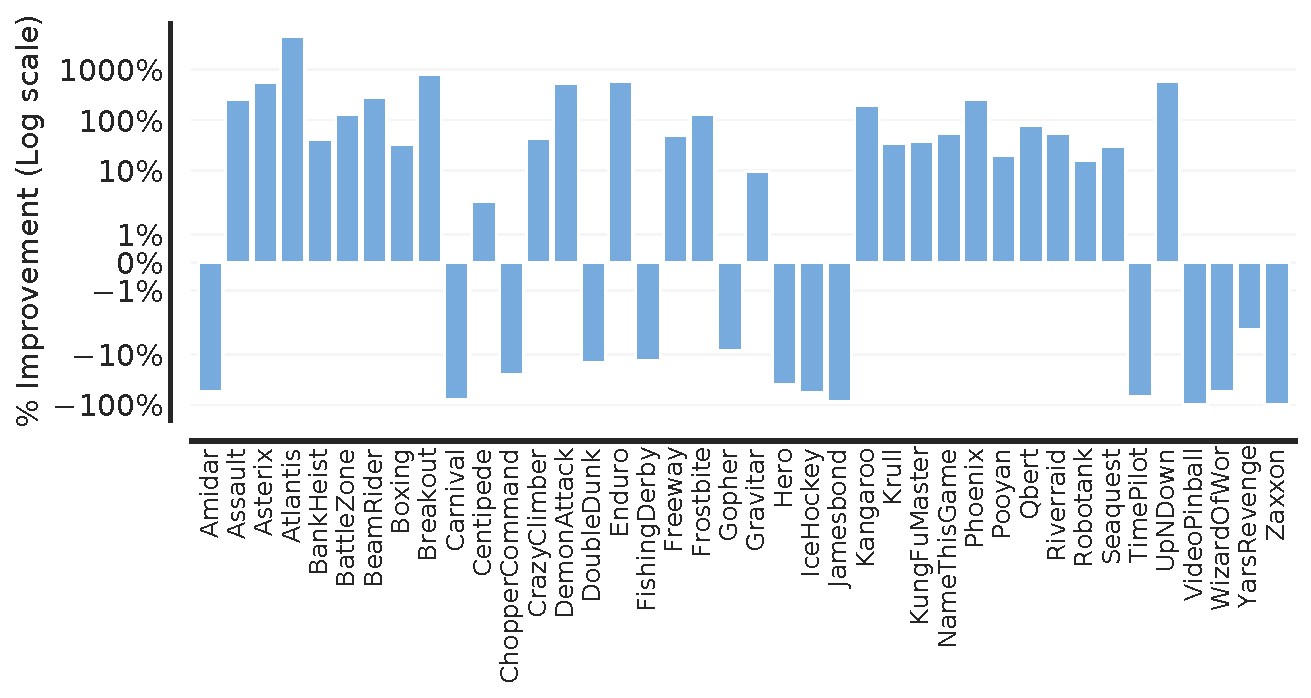
\includegraphics[width=\linewidth]{chapters/scaled_ql/figures/percent_improvement_over_DT.pdf}
    \end{minipage}
    \hfill
    \begin{minipage}{0.34\linewidth}
    \vspace{-0.2cm}
 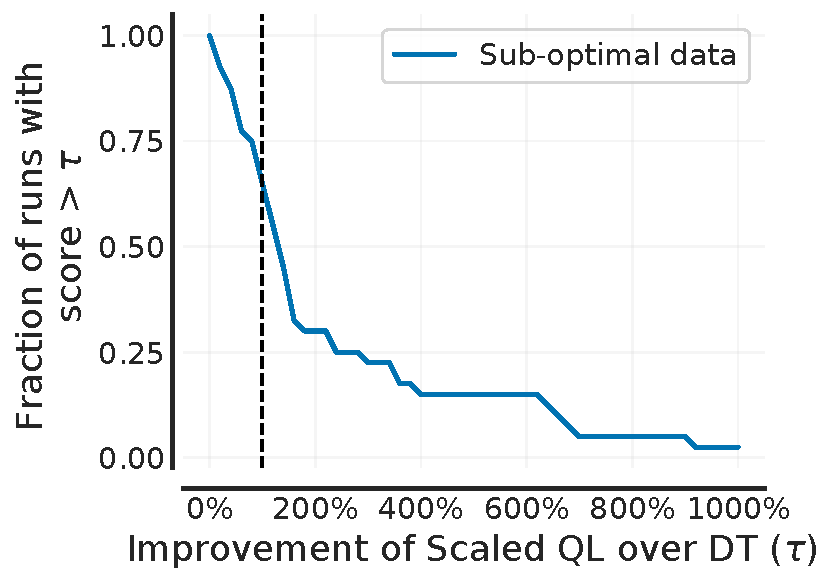
\includegraphics[width=\linewidth]{chapters/scaled_ql/figures/pp_profile_ql_dt.pdf}
    \end{minipage}
    \vspace{-0.4cm}
    \caption{\textbf{Comparing Scaled QL to DT} on all training games on the sub-optimal dataset.}
    \label{fig:percent_improvement}
    \vspace{-0.5cm}
\end{figure}

In our experiments, we study how our approach, scaled Q-learning, can simultaneously learn from sub-optimal and optimal data collected from 40 different Atari games. 
We compare the resulting multi-task policies to behavior cloning~(BC) with same architecture as scaled QL, and the prior state-of-the-art method based on decision transformers (DT)~\citep{chen2021decision}, which utilize return-conditioned supervised learning with large transformers~\citep{lee2022multi}, and have been previously proposed for addressing this task. 
We also study the efficacy of the multi-task initialization produced by scaled Q-learning in facilitating rapid transfer to new games via both offline and online fine-tuning, in comparison to state-of-the-art self-supervised representation learning methods and other prior approaches. Our goal is to answer the following questions: \textbf{(1)} How do our proposed design decisions impact performance scaling with high-capacity models?, \textbf{(2)} Can scaled QL more effectively leverage higher model capacity compared to na\"ive instantiations of Q-learning?, \textbf{(3)} Do the representations learned by scaled QL transfer to new games? We will answer these questions in detail through multiple experiments in the coming sections, but we will first summarize our main results below.


\textbf{Main empirical findings.} Our main results are summarized in Figures~\ref{fig:suboptimal_offline} and \ref{fig:main_results}. These figures show the performance of scaled QL, multi-game decision transformers~\citep{lee2022multi} (marked as ``DT''), a prior method based on supervised learning via return conditioning, and standard behavioral cloning baselines (marked as ``BC'') in the two settings discussed previously, where we must learn from: (i) near optimal data, and (ii) sub-optimal data obtained from the initial 20\% segment of the replay buffer (see our discussion about the problem setup). See Figure~\ref{fig:percent_improvement} for a direct comparison between DT and BC.


\begin{wrapfigure}{r}{0.5\linewidth}
    \vspace{-0.5cm}
    \centering
    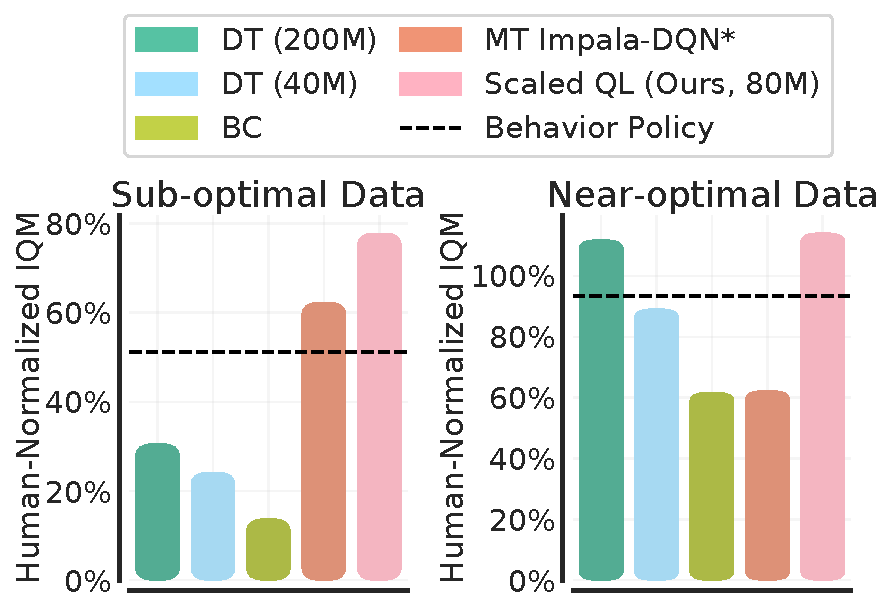
\includegraphics[width=0.95\linewidth]{chapters/scaled_ql/combnined_data_results_iqm.pdf}
    \vspace{-0.25cm}
    \caption{\footnotesize{\textbf{Offline scaled conservative Q-learning vs other prior methods} with near-optimal data and sub-optimal data. Scaled QL outperforms the best DT model, attaining an IQM human-normalized score of \textbf{114.1\%} on the near-optimal data and \textbf{77.8\%} on the sub-optimal data, compared to 111.8\% and 30.6\% for DT, respectively.}}
    \label{fig:main_results}
    \vspace{-0.5cm}
\end{wrapfigure}

In the more challenging sub-optimal data setting, scaled QL attains a performance of \textbf{77.8\%} IQM human-normalized score, although trajectories in the sub-optimal training dataset only attain 51\% IQM human-normalized score. Scaled QL also outperforms the prior DT approach by \textbf{2.5 times} on this dataset, even though the DT model has more than twice as many parameters and uses data augmentation, compared to scaled QL. 

In the $2^{nd}$ setting with near-optimal data, where the training dataset already contains expert trajectories, scaled QL with 80M parameters still outperforms the DT approach with 200M parameters, although the gap in performance is small (3\% in IQM performance, and 20\% on median performance). 
Overall, these results show that scaled QL is an effective approach for learning from large multi-task datasets, for a variety of data compositions including sub-optimal datasets, where we must stitch useful segments of suboptimal trajectories to perform well, and near-optimal datasets, where we should attempt to mimic the best behavior in the offline dataset. 

To the best of our knowledge, these results represent the largest performance improvement over the average performance in the offline dataset on such a challenging problem. We will now present experiments that show that offline Q-learning scales and generalizes.

\begin{figure}[h]
\centering
\vspace{-0.2cm}
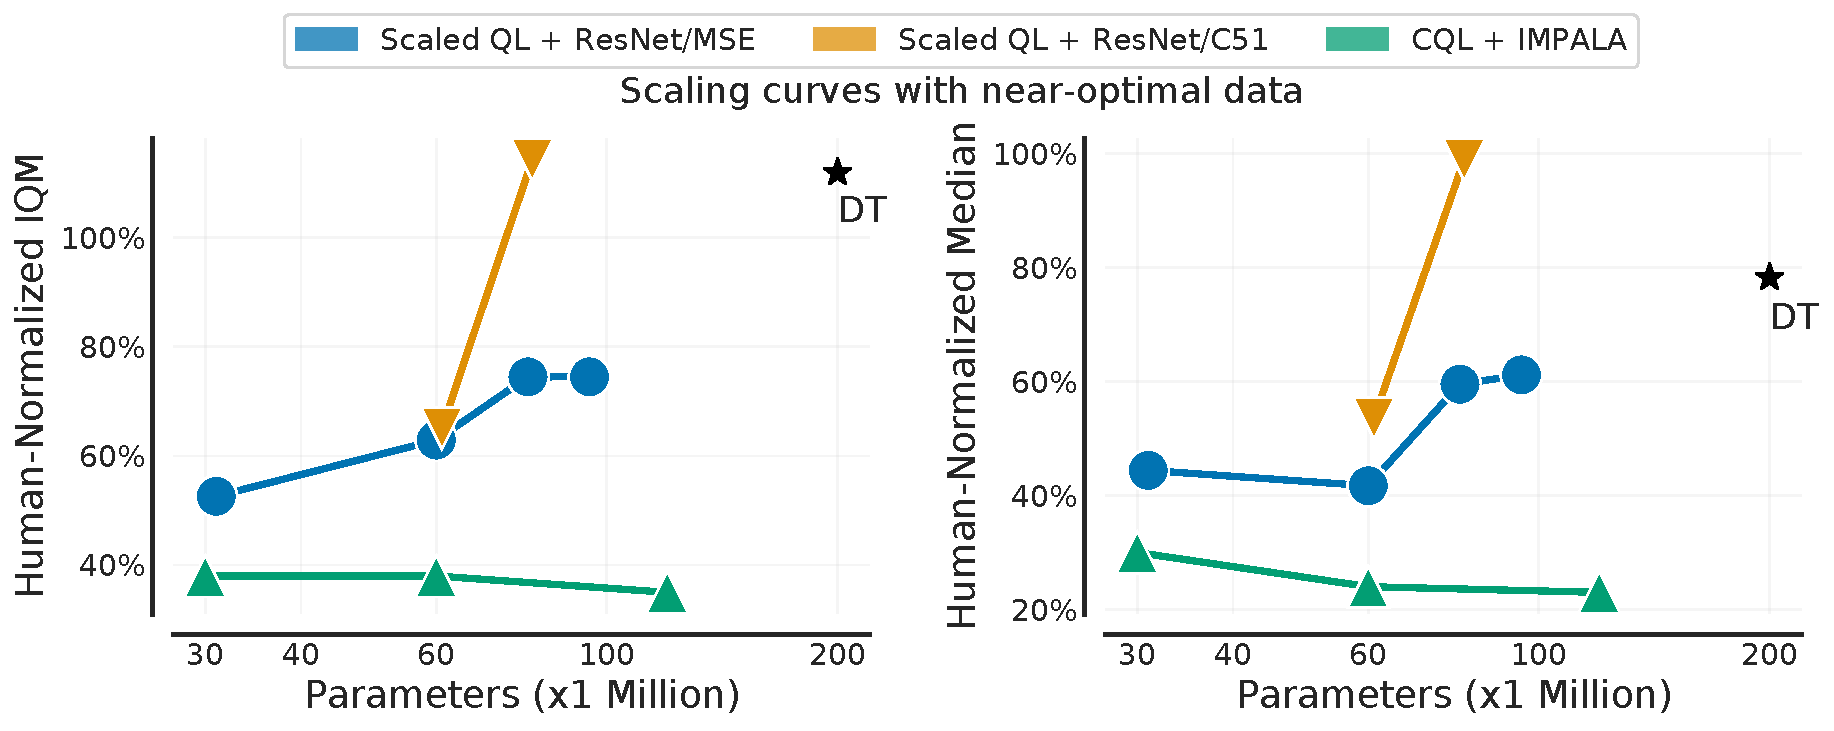
\includegraphics[width=0.75\linewidth]{chapters/scaled_ql/figures/scaling_plot_params_with_dt.pdf}
\vspace{-0.2cm}
\caption{\footnotesize{\textbf{Scaling trends for offline Q-learning.} Observe that while the performance of scaled QL instantiated with IMPALA architectures~\citep{espeholt2018impala} degrades as we increase model size, the performance of scaled QL utilizing the ResNets described in Section~\ref{sec:scaledql_method} continues to increase as model capacity increases. This is true for both an MSE-style TD error as well as for the categorical TD error used by C51 (which performs better on an absolute scale). The CQL + IMPALA performance numbers are from~\citep{lee2022multi}.}
}
\label{fig:scaling}
\vspace{-0.2cm}
\end{figure}

\vspace{-0.2cm}
\subsubsection{Does Offline Conservative Q-Learning Scale Favorably?}
\vspace{-0.2cm}
One of the primary goals of this chapter was to understand if scaled Q-learning is able to leverage the benefit of higher capacity architectures. Recently, \citet{lee2022multi} found that the performance of CQL with the IMPALA architecture does not improve with larger model sizes and may even degrade with larger model sizes. To verify if scaled Q-learning can address this limitation, we compare our value-based offline RL approach with a variety of model families: \textbf{(a)} IMPALA family~\citep{espeholt2018impala}: three IMPALA models with varying widths ($4, 8, 16$) whose performance numbers are taken directly from \citet{lee2022multi} (and was consistent with our preliminary experiments), 
%%AK: check if this is the standard naming or not?
\textbf{(b)} ResNet 34, 50, 101 and 152 from the ResNet family, modified to include group normalization and learned spatial embeddings.%, and \textbf{(c)} ViT-Base and ViT-Large from the vision transformer family, similar to decision transformers. 
These architectures include both small and large networks, spanning a wide range from 1M to 100M parameters. As a point of reference, we use the scaling trends of the multi-game decision transformer and BC approaches from \citet{lee2022multi}.
%%SL.9.27: if we don't end up including vit, make sure to revise the above discussion

Observe in Figure~\ref{fig:scaling} that the performance of scaled Q-learning improves as the underlying Q-function model size grows. Even though the standard mean-squared error formulation of TD error results in worse absolute performance than C51 (blue vs orange), for both of these versions, the performance of scaled Q-learning increases as the models become larger. This result indicates that value-based offline RL methods can scale favorably, and give rise to better results, but this requires carefully picking a model family. This also explains the findings from \citet{lee2022multi}: while this prior work observed that CQL with IMPALA scaled poorly as model size increases, they also observed that the performance of return-conditioned RL instantiated with IMPALA architectures also degraded with higher model sizes. Combined with the results in Figure~\ref{fig:scaling} above, this suggests that poor scaling properties of offline RL can largely be attributed to the choice of IMPALA architectures, which may not work well in general even for supervised learning methods (like return-conditioned BC).


\vspace{-0.2cm}
\subsubsection{Can Offline RL Learn Useful Initializations that Enable Fine-Tuning?}
\label{sec:ft_off_on}
\vspace{-0.2cm}

Next, we study how multi-task training on multiple games via scaled QL can learn general-purpose representations that can enable \emph{rapid} fine-tuning to new games. We study this question in two scenarios: fine-tuning to a new game via offline RL with a small amount of held-out data (1\% uniformly subsampled datasets from DQN-Replay~\citep{agarwal2019optimistic}), and finetuning to a new game mode via sample-efficient online RL initialized from our multi-game offline Q-function. For finetuning, we transfer the weights from the visual encoder and reinitialize the downstream feed-forward component (Figure~\ref{fig:overview}). For both of these scenarios, we utilize a ResNet101 Q-function trained via the methodology in Section~\ref{sec:scaledql_method}, using C51 and feature normalization.

\begin{figure}[t]
    \centering
    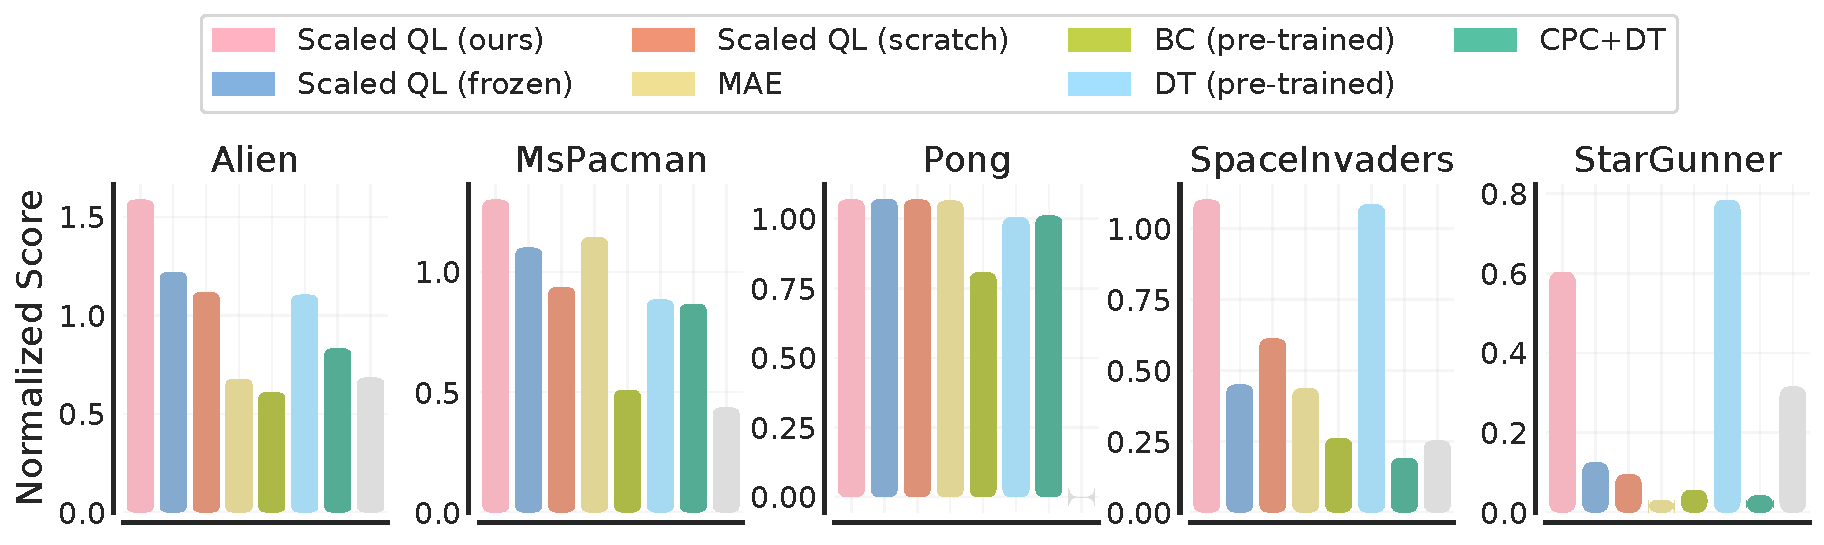
\includegraphics[width=0.99\linewidth]{chapters/scaled_ql/figures/offline_ft.pdf}
    \vspace{-0.25cm}
    \caption{\footnotesize{\textbf{Offline fine-tuning} performance on unseen games trained with 1\% of held-out game's data, measured in terms of DQN-normalized score, following \citep{lee2022multi}. On average, pre-training with scaled QL outperforms other methods by \textbf{82\%}. Furthermore, scaled QL improves over scaled QL (scratch) by 45\%, indicating that the representations learned by scaled QL during multi-game pre-training are useful for transfer. Self-supervised representation learning (CPC, MAE) alone does not attain good fine-tuning performance.}}
    \label{fig:offline_ft}
    \vspace{-0.3cm}
\end{figure}
%%AK: not having baselines para here, since the comparisons are different

\textbf{Scenario 1 (Offline fine-tuning)}: First, we present the results for fine-tuning in an offline setting: following the protocol from \citet{lee2022multi}, we use the pre-trained representations to rapidly learn a policy for a novel game using limited offline data (1\% of the experience of an online DQN run). In Figure~\ref{fig:offline_ft}, we present our results for offline fine-tuning on 5 games from \citet{lee2022multi}, \textsc{Alien, MsPacman, Space Invaders, StarGunner} and \textsc{Pong}, alongside the prior approach based on decision transformers (``DT (pre-trained)''), and fine-tuning using pre-trained representations learned from state-of-the-art self-supervised representation learning methods such as contrastive predictive coding (CPC)~\citep{oord2018representation} and masked autoencoders (MAE)~\citep{he2111masked}. For CPC performance, we use the baseline reported in \citet{lee2022multi}. MAE is a more recent self-supervised approach that we find generally outperformed CPC in this comparison. For MAE, we first pretrained a vision transformer~(ViT-Base)~\citep{dosovitskiy2020image} encoder with 80M parameters trained via a reconstruction loss on observations from multi-game Atari dataset and freeze the encoder weights as done in prior work~\citep{xiao2022masked}. 
Then, with this frozen visual encoder, we used the same feed forward architecture, Q-function parameterization, and training objective (CQL with C51) as scaled QL to finetune the MAE network. We also compare to baseline methods that do not utilize any multi-game pre-training (DT (scratch) and Scaled QL (scratch)). 

\textbf{Results.} Observe in Figure~\ref{fig:offline_ft} that multi-game pre-training via scaled QL leads to the best fine-tuning performance and improves over prior methods, including decision transformers trained from scratch. %, by XX\% in aggregate. 
Importantly, we observe \emph{positive transfer} to new games via scaled QL. Prior works~\citep{badia2020agent57}
running multi-game Atari (primarily in the online setting) have generally observed negative transfer across Atari games. We show for the first time that pre-trained representations from Q-learning enable positive transfer to novel games that significantly outperforms return-conditioned supervised learning methods and dedicated representation learning approaches.

\textbf{Scenario 2 (Online fine-tuning)}: Next, we study the efficacy of the learned representations in enabling online fine-tuning. While deep RL agents on ALE are typically trained on default game modes~(referred to as $m0d0$), we utilize new \emph{variants} of the ALE games designed to be challenging for humans~\citep{machado18sticky} for online-finetuning. We investigate whether multi-task training on the 40 default game variants can enable fast online adaptation to these never-before-seen variants. In contrast to offline fine-tuning (Scenario 1), this setting tests whether scaled QL can also provide a good initialization for online data collection and learning, for closely related but different tasks. Following \citet{farebrother2018generalization}, we use the same \emph{variants} investigated in this prior work: $\textsc{Breakout}$, $\textsc{Hero}$, and $\textsc{Freeway}$, which we visualize in Figure~\ref{fig:online_ft}~(left).
To disentangle the performance gains from multi-game pre-training and the choice of Q-function architecture, we compare to a baseline approach (``scaled QL (scratch)'') that utilizes an identical Q-function architecture as pre-trained scaled QL, but starts from a random initialization. As before, we also evaluate fine-tuning performance using the representations obtained via masked auto-encoder pre-training~\citep{he2111masked,xiao2022masked}. We also compare to a single-game DQN performance attained after training for 50M steps, $16\times$ more transitions than what is allowed for scaled QL, as reported by \citet{farebrother2018generalization}.

\textbf{Results}. Observe in Figure~\ref{fig:online_ft} that fine-tuning from the multi-task initialization learned by scaled QL significantly outperforms training from scratch as well as the single-game DQN run trained with \textbf{16x} more data. Fine-tuning with the frozen representations learned by MAE performs poorly, which we hypothesize is due to differences in game dynamics and subtle changes in observations, which must be accurately accounted for in order to learn optimal behavior~\citep{dean2022don}. Our results confirm that offline Q-learning can both effectively benefit from higher-capacity models and learn multi-task initializations that enable sample-efficient transfer to new games. 


\begin{figure}[t]
    \centering
        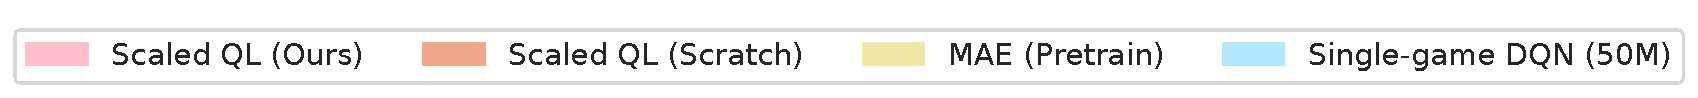
\includegraphics[width=0.9\linewidth]{chapters/scaled_ql/figures/legend_online_ft.pdf}
        \vspace{-0.1cm}
        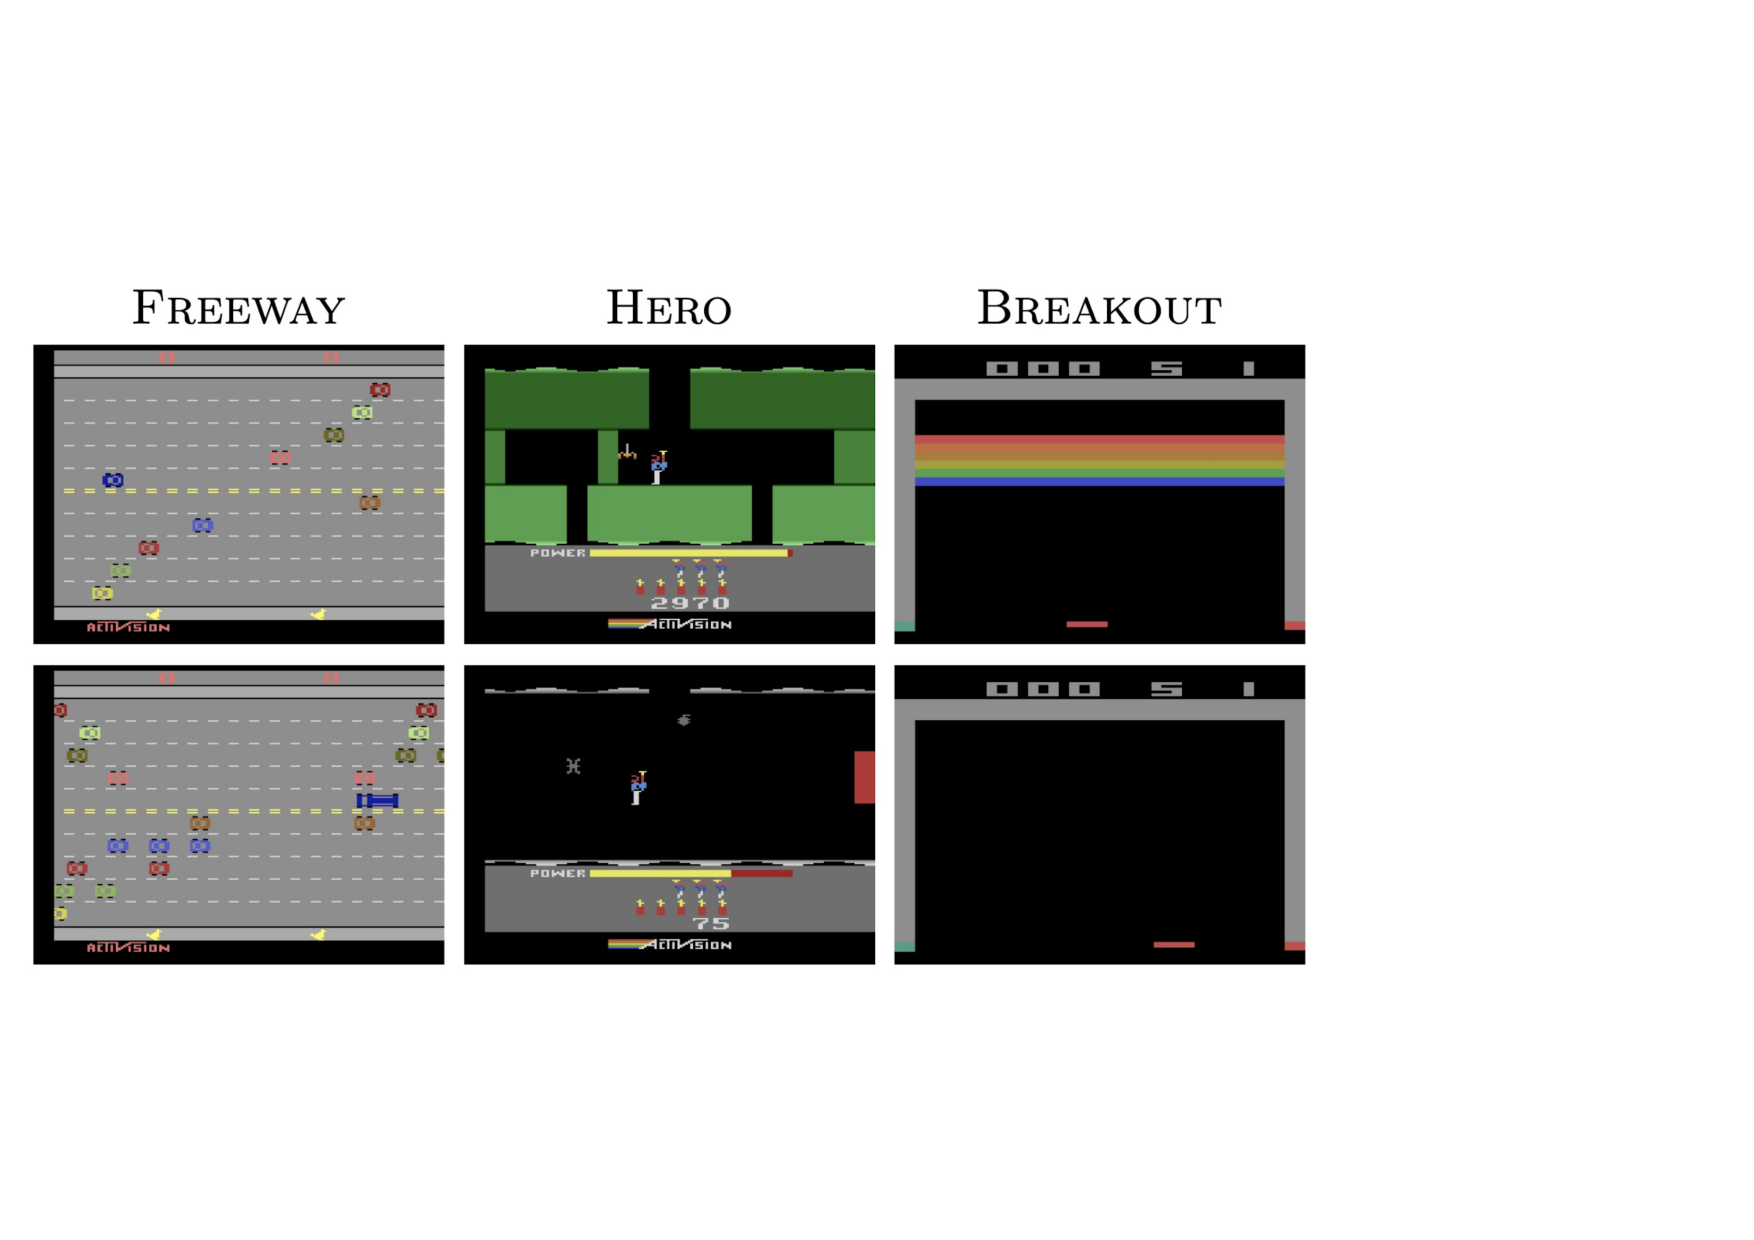
\includegraphics[width=0.35\linewidth]{chapters/scaled_ql/figures/atari_modes_3games.pdf}
        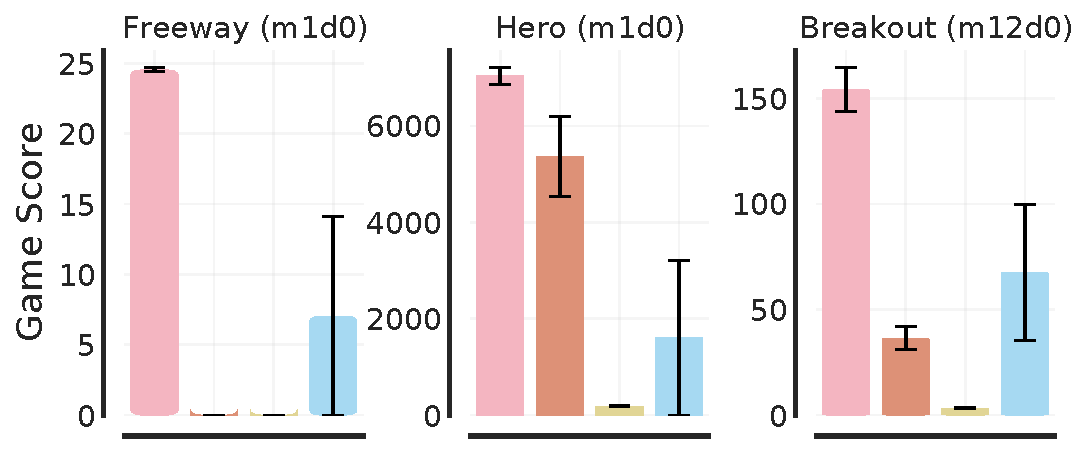
\includegraphics[width=0.5\linewidth]{chapters/scaled_ql/figures/online_ft_3_games.pdf}
    \vspace{-0.1cm}
    \caption{\footnotesize{\textbf{Online fine-tuning} results on unseen game \emph{variants}. \textbf{Left}. The top row shows default variants and the bottom row shows unseen variants evaluated for transfer: Freeway’s mode 1 adds buses, more vehicles, and increases velocity; Hero’s mode 1 starts the agent at level 5; Breakout’s mode 12 hides all bricks unless the ball has recently collided with a brick. \textbf{Right}. We fine-tune all methods except single-game DQN for 3M online frames (as we wish to test fast online adaptation). Error bars show minimum and maximum scores across 2 runs while the bar shows their average. Observe that scaled QL significantly outperforms learning from scratch and single-game DQN with 50M online frames. Furthermore, scaled QL also outperforms RL fine-tuning on representations learned using masked auto-encoders. See Figure~\ref{fig:lr_curves_online_ft} for learning curves.}}
    \label{fig:online_ft}
    \vspace{-0.5cm}
\end{figure}


\vspace{-0.25cm}
\subsubsection{Ablation Studies}
\label{sec:ablation}
\vspace{-0.25cm}

Finally, in this section we perform controlled ablation studies to understand how crucial the design decisions introduced in Section~\ref{sec:scaledql_method} are for the success of scaled Q-learning. In particular, we will attempt to understand the benefits of using C51 and feature normalization.

\textbf{MSE vs C51:} We ran scaled Q-learning with identical network architectures (ResNet 50 and ResNet 101), with both the conventional squared error formulation of TD error, and compare it to C51, which our main results utilize. Observe in Table~\ref{tab:ablation_mse} that C51 leads to much better performance for both ResNet 50 and ResNet 101 models. The boost in performance is the largest for ResNet 101, where C51 improves by over \textbf{39\%} as measured by median human-normalized score. This observation is surprising since prior work~\citep{agarwal2021deep} has shown that C51 performs on par with standard DQN with an Adam optimizer, which all of our results use. One hypothesis is that this could be the case as TD gradients would depend on the scale of the reward function, and hence some games would likely exhibit a stronger contribution in the gradient. This is despite the fact that our implementation of MSE TD-error already attempts to correct for this issue by applying the unitary scaling technique from \citep{kurin2022defense} to standardize reward scales across games. That said, we still observe that C51 performs significantly better.

\begin{table}[t]
    \centering
% \fontsize{8}{8}\selectfont
    \centering
    \vspace{-0.3cm}
    \caption{\footnotesize{\textbf{Performance of Scaled QL with the standard mean-squared TD-error and C51} in the offline 40-game setting aggregated by the median human-normalized score. Observe that for both ResNet 50 and ResNet 101, utilizing C51 leads to a drastic improvement in performance.}}% (as large as 39.4\% improvement on human-median normalized score with ResNet 101).}}
    \label{tab:ablation_mse}
    \vspace{0.1cm}
\resizebox{0.6\linewidth}{!}{\begin{tabular}{lcc}
\toprule
 & \textbf{Scaled QL (ResNet 50)} & \textbf{Scaled QL (ResNet 101)} \\
\midrule
\textbf{with MSE}  &  41.1\% & 59.5\%  \\
\midrule
\textbf{with C51}  & 53.5\% (+12.4\%) & 98.9\% (+39.4\%) \\
\bottomrule
\vspace{-0.25in}
\end{tabular}}
\end{table}


\textbf{Importance of feature normalization:} We ran small-scale experiments with and without feature normalization (Section~\ref{sec:scaledql_method}). In these experiments, we consider a multi-game setting with only 6 games: \textsc{Asterix}, \textsc{Breakout}, \textsc{Pong}, \textsc{SpaceInvaders}, \textsc{Seaquest}, and we train with the initial 20\% data for each game. We report aggregated median human-normalized score across the 6 games in Table~\ref{tab:ablation_dr3} for three different network architectures (ResNet 34, ResNet 50 and ResNet 101). Observe that the addition of feature normalization significantly improves performance for all the models. Motivated by this initial empirical finding, we used feature normalization in all of our main experiments. Overall, the above ablation studies validate the efficacy of the two key design decisions in this chapter. 
% However, there are several avenues for future investigation: 1) it is unclear if C51 works better because of the distributional formulation or the categorical representation and experiments with other distributional formulations could answer this question, 2) we did not extensively try alternate feature normalization schemes which may improve results. 

\begin{table}[ht]
    \centering
% \fontsize{8}{8}\selectfont
    \centering
    \vspace{-0.2cm}
    \caption{\footnotesize{\textbf{Performance of Scaled QL with and without feature normalization in the 6 game setting} reported in terms of the median human-normalized score. Observe that with models of all sizes, the addition of feature normalization improves performance.}}
    \label{tab:ablation_dr3}
    \vspace{0.1cm}
\resizebox{\linewidth}{!}{\begin{tabular}{lccc}
\toprule
 & \textbf{Scaled QL (ResNet 34)} & \textbf{Scaled QL (ResNet 50)} & \textbf{Scaled QL (ResNet 101)} \\
\midrule
\textbf{without feature normalization}  &  50.9\%  & 73.9\% & 80.4\%    \\
\midrule
\textbf{with feature normalization}  & 78.0\% (+28.9\%)  & 83.5\% (+9.6\%)  & 98.0\% (+17.6\%) \\
\bottomrule
\vspace{-0.2in}
\end{tabular}
}
\end{table}

\textbf{Additional ablations:} We also conducted ablation studies for the choice of the backbone architecture (spatial learned embeddings) in Appendix~\ref{app:backbone_ablation}, and observed that utilizing spatial embeddings is better. We also evaluated the performance of scaled QL without conservatism to test the importance of utilizing pessimism in our setting with diverse data in Appendix~\ref{app:no_pessimism}, and observe that pessimism is crucial for attaining good performance on an average. We also provide some scaling studies for another offline RL method (discrete BCQ) in Appendix~\ref{app:discrete_bcq}.



\vspace{0.1cm}
\section{Discussion and Conclusion}
\label{sec:conclusion}
\vspace{0.1cm}
We presented a system that uses diverse prior data for general-purpose offline RL pre-training, followed by fine-tuning to downstream tasks. The prior data, sourced from a publicly available dataset, consists of over a hundred tasks across ten scenes and our policies can be fine-tuned with as few as 10 demonstrations. We show that this approach outperforms prior pre-training and fine-tuning methods based on imitation learning. One of the most exciting directions for future work is to further scale up this pre-training to provide a single policy initialization, that can be utilized as a starting point, similar to GPT3~\citep{brown2020language}. 
An exciting future direction is to scale PTR up to more complex settings, including to novel robots. {Since joint training with offline RL was worse than pre-training and then fine-tuning with PTR, another exciting direction for future work is to understand the pros and cons of joint training and fine-tuning in the context of robot learning.}

\vspace{0.1cm}

% \clearpage


%===============================================================================

% The maximum paper length is 8 pages excluding references and acknowledgements, and 10 pages including references and acknowledgements


% The acknowledgments are automatically included only in the final and preprint versions of the paper.
%\acknowledgments{todo!}

%===============================================================================

% no \bibliographystyle is required, since the corl style is automatically used.
% \bibliography{example}  % .bib


\bibliography{main}
\bibliographystyle{plainnat}


\newpage
\clearpage
\appendix

\subsection{Diagnostic study in simulation}
\label{app:sim_diagnostic}
 We perform a diagnostic study in simulation to verify some of the insights observed in our real-world experiments. We created a bin sort task, where a WidowX250 robot is placed in front two bins and is provided with two objects (more details in Appendix~\ref{app:exp_setup}). The task is to sort each object in the correct bin associated with that object. The pre-training data provided to this robot is pick-place data, which only demonstrates how to pick \emph{one} of the objects and place it in one of the bins, but does not demonstrate the compound task of placing both objects. In order to succeed at this such a compound task, a robot must learn an abstract representation of the skill of sorting an object during the pre-training phase and then figure out that it needs to apply this skill multiple times in a trajectory to succeed at the task from just \emph{five} demonstrations of the desired sorting behavior.


The performance numbers (along with 95\%-confidence intervals) are shown in Table~\ref{tab:sim_complete}. Observe that \methodname improves upon prior methods in a statistically significant manner, outperforming the BC and COG baselines by a significant margin. This validates the efficacy of \methodname in simulation and corroborates our real-world results. 


\begin{table}[h]
\centering
\begin{tabular}{l|r}
\toprule
\textbf{Method} & \textbf{Success rate}  \\ \midrule
BC (joint training) & 7.00 $\pm$ 0.00 \% \\
COG (joint training) & 8.00 $\pm$ 1.00 \% \\
BC (finetune) & 4.88 $\pm$ 4.07 \% \\ \midrule
\textbf{\methodname (Ours)} & \textbf{17.41 $\pm$ 1.77 \%} \\
\bottomrule
\end{tabular}
\caption{\label{tab:sim_complete} \footnotesize{\textbf{Performance of \methodname in comparison with other methods} on the simulated bin sorting task, trained for many more gradient steps for all methods until each one of them converges. Observe that \methodname substantially outperforms other prior methods, including joint training on the same data with BC or CQL. Training on target data only is unable to recover a non-zero performance, so we do not report it in this table. Since the 95\%-confidence intervals do not overlap between \methodname and other methods, it indicates that \methodname improves upon baselines in a statistically significant manner.}}
\end{table}



\subsection{Details of Our Experimental Setup}
\label{app:exp_setup}

\vspace{0.1cm}
\subsubsection{Real-World Experimental Setup}

A picture of our real-world experimental setup is shown in Figure \ref{fig:setup_overview}. The scenarios considered in our experiments (Section~\ref{sec:result}) are designed to evaluate the performance of our method under a variety of situations and therefore we set up these tasks in different toykitchen domains (see Figure \ref{fig:setup_overview}) on three different WidowX 250 robot arms. We use data from the bridge dataset~\citep{ebert2021bridge} consisting of data collected with many robots in many domains for training but exclude the task/domain that we use for evaluation from the training dataset.  

\begin{figure}[h]
\centering
  \includegraphics[width=\linewidth]{setup_overview.pdf}
  \caption{\footnotesize{\textbf{Setup Overview}: Following \citet{ebert2021bridge}, we use a toykitchen setup described in that prior work for our experiments. This utilizes a 6-DoF WidowX 250 robot. \textbf{(1):}  Held-out toykitchen used for experiments in Scenario 3 (denoted ``toykitchen 6''), \textbf{(2):}  Re-targeting toykitchen used for experiments in Scenario 2 (denoted ``toykitchen 2''), \textbf{(3):} target objects used in the experiments of scenario 3.}, \textbf{(4):} the held-out kitchen setup used for door opening (``toykitchen 1'').}
  \label{fig:setup_overview}
  \vspace{-0.3cm}
\end{figure}



\subsubsection{Diagnostic Experimental Setup in Simulation}
\label{sec:sim_appendix}

\begin{figure}{}
\centering
    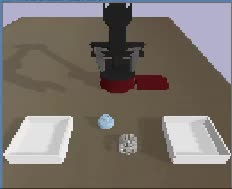
\includegraphics[width=0.8\linewidth]{binsort_figure.jpg}
  \caption{\footnotesize{\textbf{Bin-Sorting task used for our simulated evaluations.} The task requires sorting the cylinder into the left bin and the teapot into the right bin.}}
  \label{app:sim_setup}
\end{figure}

We evaluate our approach in a simulated bin-sorting task on the simulated WidowX 250 platform, aimed to mimic the setup we use for our real-world evaluations. This setup is designed in the PyBullet simulation framework provided by \citet{singh2020cog}. A picture is shown in Figure \ref{app:sim_setup}. In this task, two different bins and two different objects are placed in front of the WidowX robot. The goal of the robot is to correctly sort each of the two objects to their designated bin (e.g the cylinder is supposed to be placed in the left bin and the teapot should be placed in the right bin. We refer to this task as a \emph{compound} task since it requires successfully combining behaviors of two different pick-and-place skills one after the other in a single trajectory while also adequately identifying the correct bin associated with each object. Success is counted only when the robot can accurately sort \emph{both} of the objects into their corresponding bins.

\textbf{Offline pre-training dataset.} The dataset provided for offline pre-training only consists of demonstrations that show how the robot should pick one of the two objects and place it into one of the two bins. Each episode in the pre-training dataset is about 30-40 timesteps long. A picture showing some trajectories from the pre-training dataset is shown in Figure \ref{fig:app_pretrain_rollout_sim}. While the downstream task only requires solving this sorting task with two specific objects (shown in Figure \ref{fig:app_targ_rollout_sim}), the pre-training data consists of 10 unique objects (some shown in Figure \ref{fig:app_pretrain_rollout_sim}). The two target objects that appear together in the downstream target scene are never seen together in the pre-training data. Since the pre-training data only demonstrates how the robot must pick up one of the objects and place it in one of the two bins (not necessarily in the target bin that the target task requires), it neither consists of any behavior that places objects into bins sequentially nor does it consist of any behavior where one of the objects is placed one of the bins while the other one is not. This is what makes this  task particularly challenging.

\textbf{Target demonstration data.} The target task data provided to the algorithm consists of only \textbf{\emph{five}} demonstrations that show how the robot must complete both the stages of placing both objects (see Figure \ref{fig:app_targ_rollout_sim}). Each episode in the target demonstration data is 80 timesteps long, which is substantially longer than any trajectory in the pre-training data, though one would hope that good representations learned from the pick and place tasks are still useful for this target task. While all methods are able to generally solve the first segment of placing the first object into the correct bin, the primary challenge in this task is to effectively sort the second object, and we find that \methodname attains a substantially better success rate than other baselines in this exact step.  

\begin{figure*}
\centering
  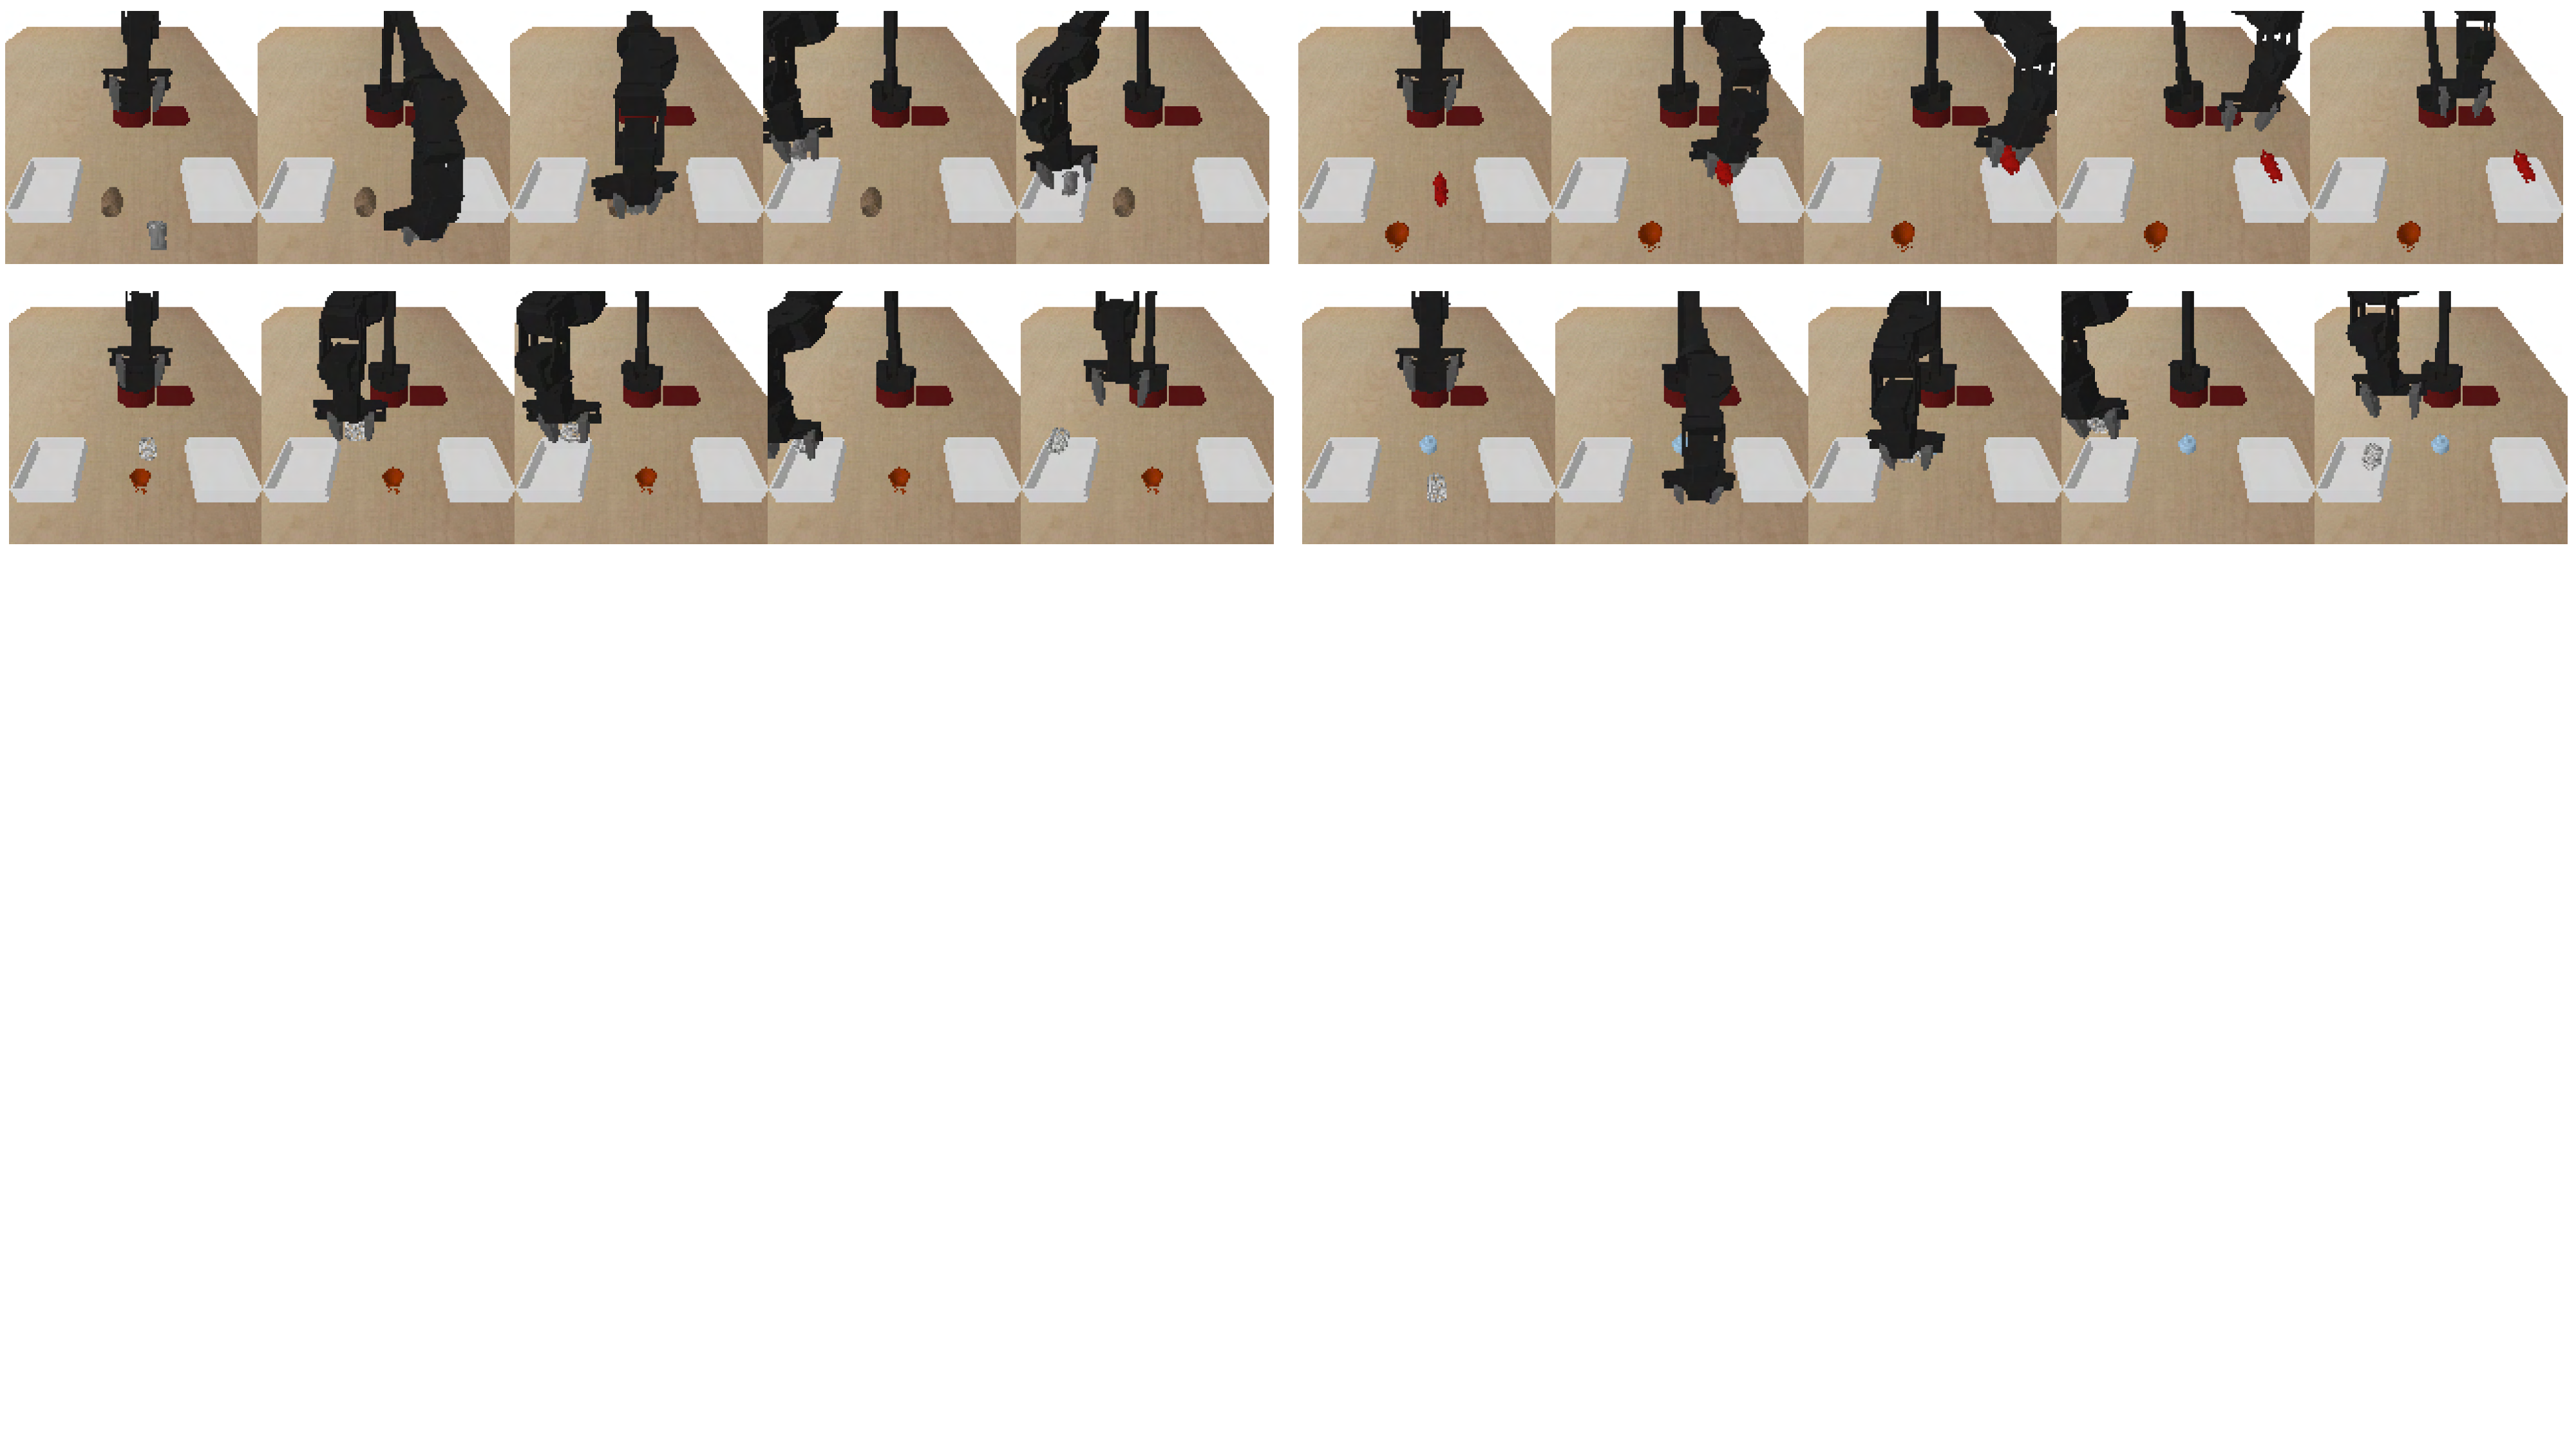
\includegraphics[width=\textwidth]{BinsortPretrainTrajAppendix.pdf}
  \caption{\label{fig:app_pretrain_rollout_sim} \footnotesize {Some trajectories from the pre-training data used in the simulated bin-sort task.}}
\end{figure*}

\begin{figure*}
\centering
  \includegraphics[width=\textwidth]{BinsortTargetTrajAppendix.pdf}
  \caption{\label{fig:app_targ_rollout_sim} \footnotesize {The five demonstration trajectories used for Phase 2 of \methodname.}}
\end{figure*}

\subsection{Description of the Real-World Evaluation Scenarios}
\label{app:tasks}
In this section, we describe the real-world evaluation scenarios considered in Section~\ref{sec:result}. We additionally include a much more challenging version of Scenario 3, for which we present results in Appendix~\ref{app:exp_results}. These harder test cases evaluate the fine-tuning performance on four different tasks, starting from the same initialization trained on bridge data except the toykitchen 6 domain in which these four tasks were set up. In the following sections, the nomenclature for the toy kitchens is drawn from \citet{ebert2021bridge} and as described in the caption of Figure~\ref{fig:setup_overview}.

\subsubsection{Scenario 1: Re-targeting skills for existing to solve new tasks}

\begin{figure}
\centering
  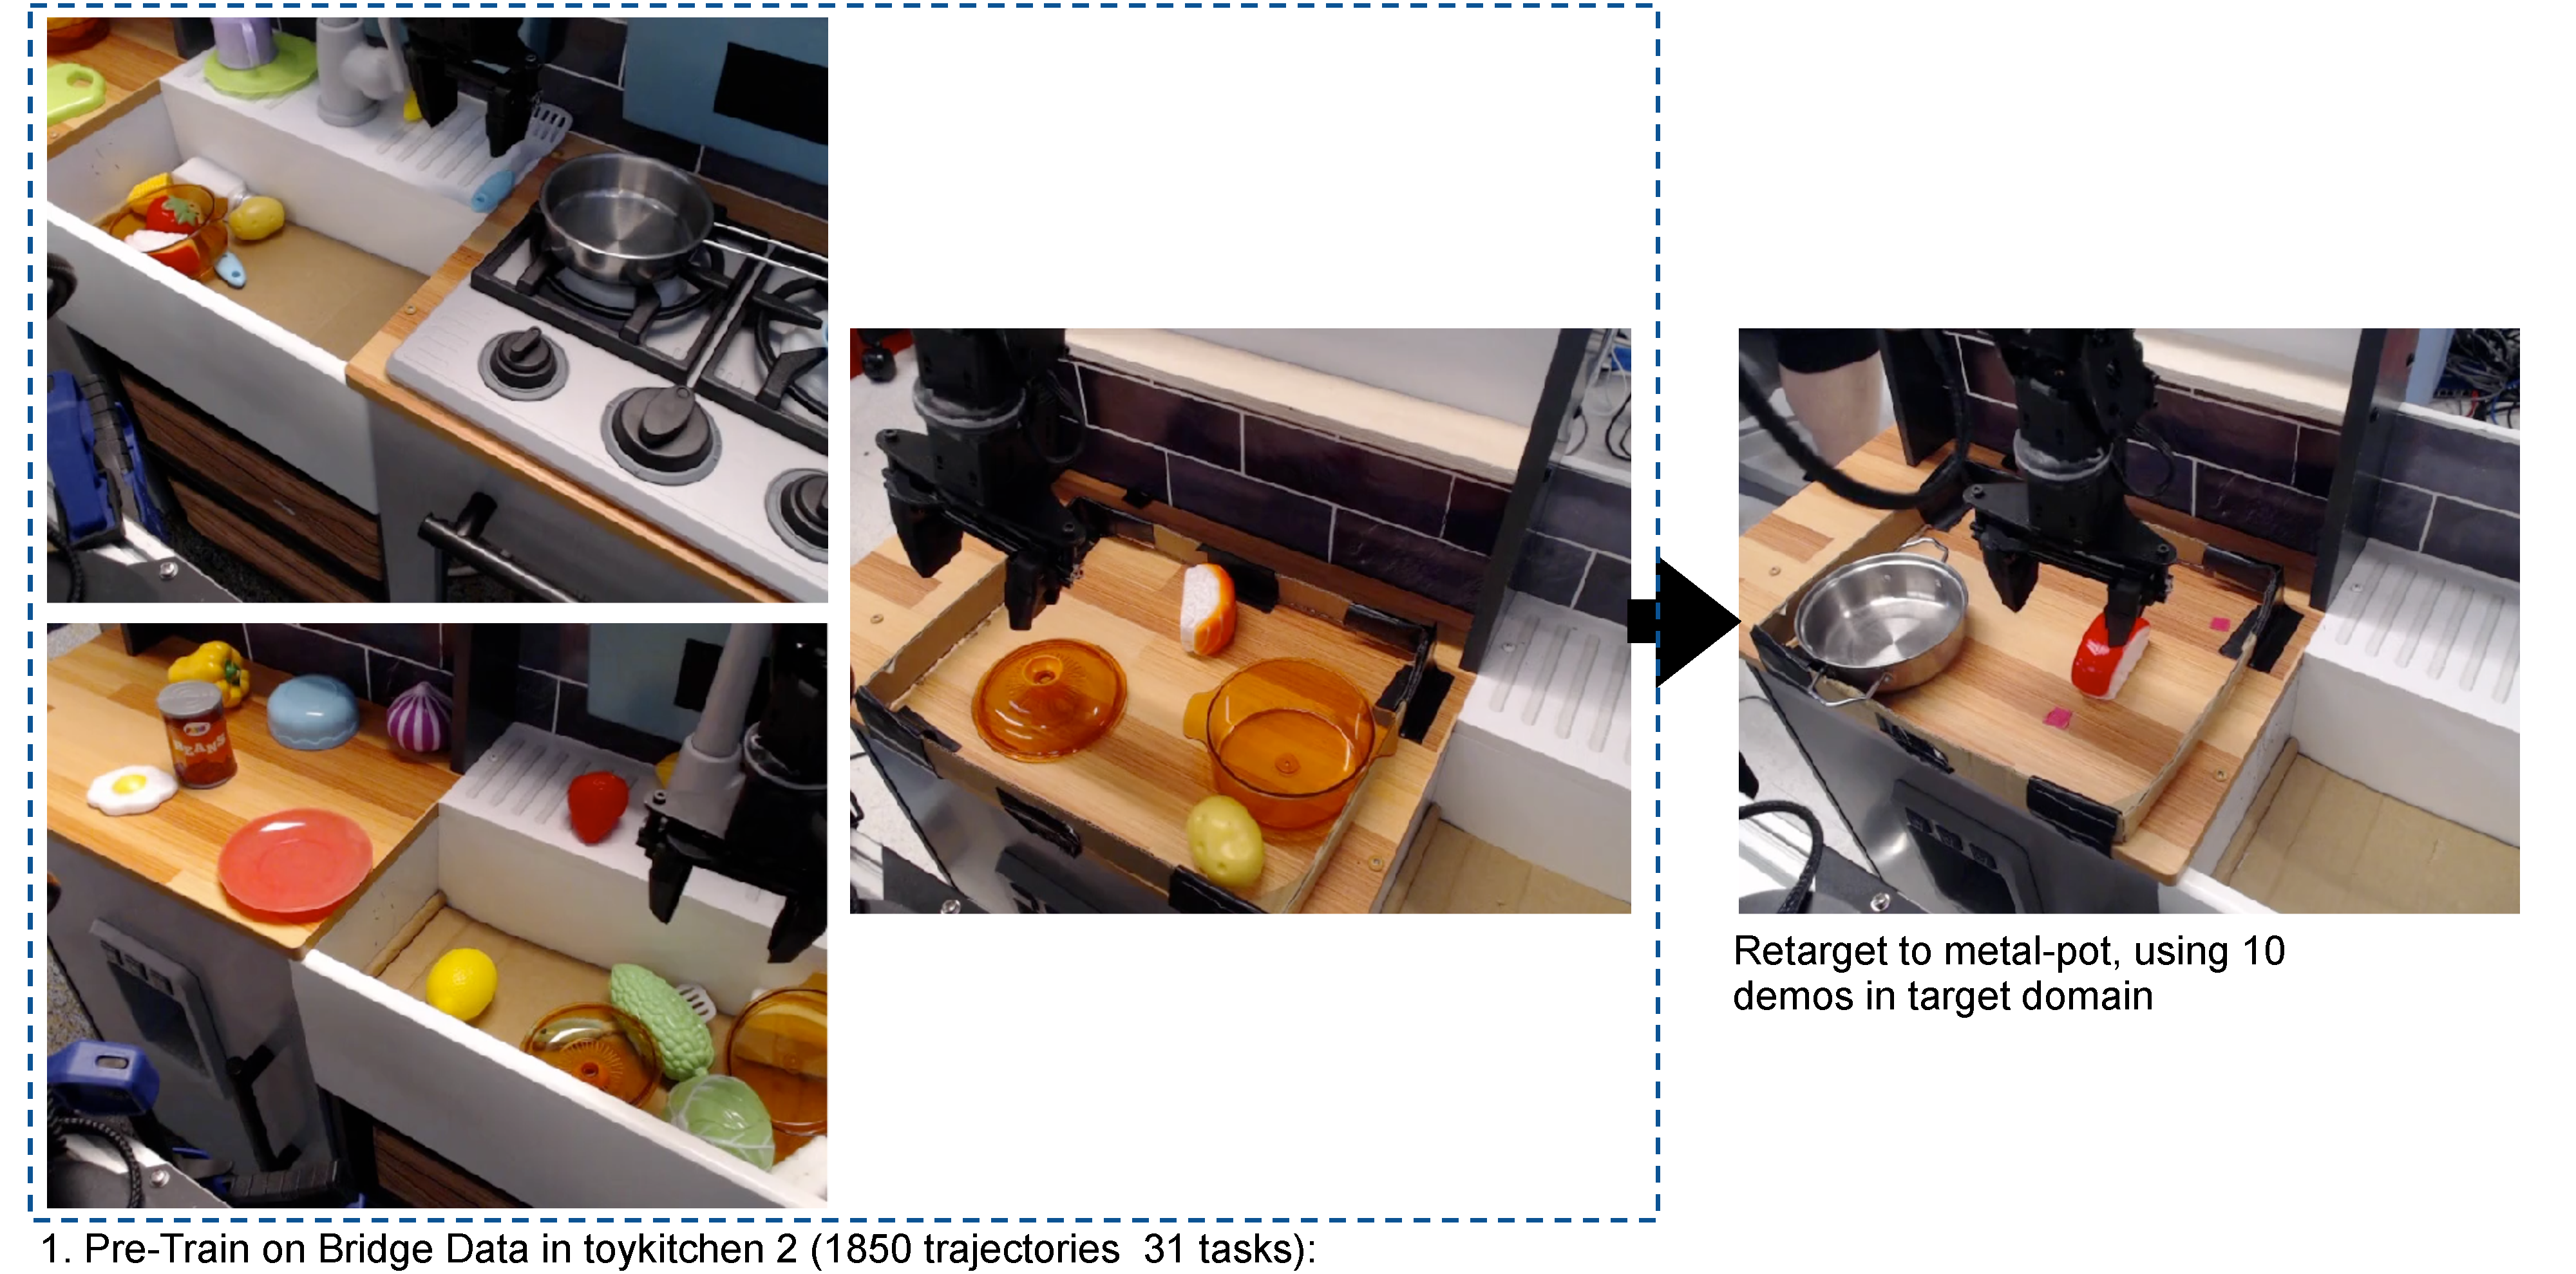
\includegraphics[width=0.83\linewidth]{scenario1_overview.pdf}
  \caption{\footnotesize \textbf{Illustration of pre-training data and finetuning data used for Scenario 1}: re-targeting the put sushi in metal-pot behavior to put the object in the metal pot instead of the orange transparent pot.}
  \label{fig:retargeting_setup}
\end{figure}


\textbf{Pre-training data.} The pre-training data comprises all of the pick and place data from the bridge dataset~\citep{ebert2021bridge} from toykitchen 2. This includes data corresponding to the task of putting the sushi in the transparent orange pot (Figure \ref{fig:retargeting_setup}).  

\textbf{Target task and data.} Since our goal in this scenario is to re-target the skill for putting the sushi in the transparent orange pot to the task of putting the sushi in the metallic pot, we utilize a dataset of 20 demonstrations that place the sushi in a metallic pot as our target task data that we fine-tune with (shown in Figure~\ref{fig:retargeting_setup}). 

\textbf{Quantitative evaluation protocol.} For our quantitative evaluations in Table \ref{tab:retarget}, we run 10 controlled evaluation rollouts that place the sushi and the metallic pot in different locations of the workspace. In all runs, the arm starts at up to 10 cm distance above the target object. The initial object and arm poses and positions are matched as closely as possible for different methods.

\subsubsection{Scenario 2: Generalizing to Previously Unseen Domains}

\begin{figure}
\centering
  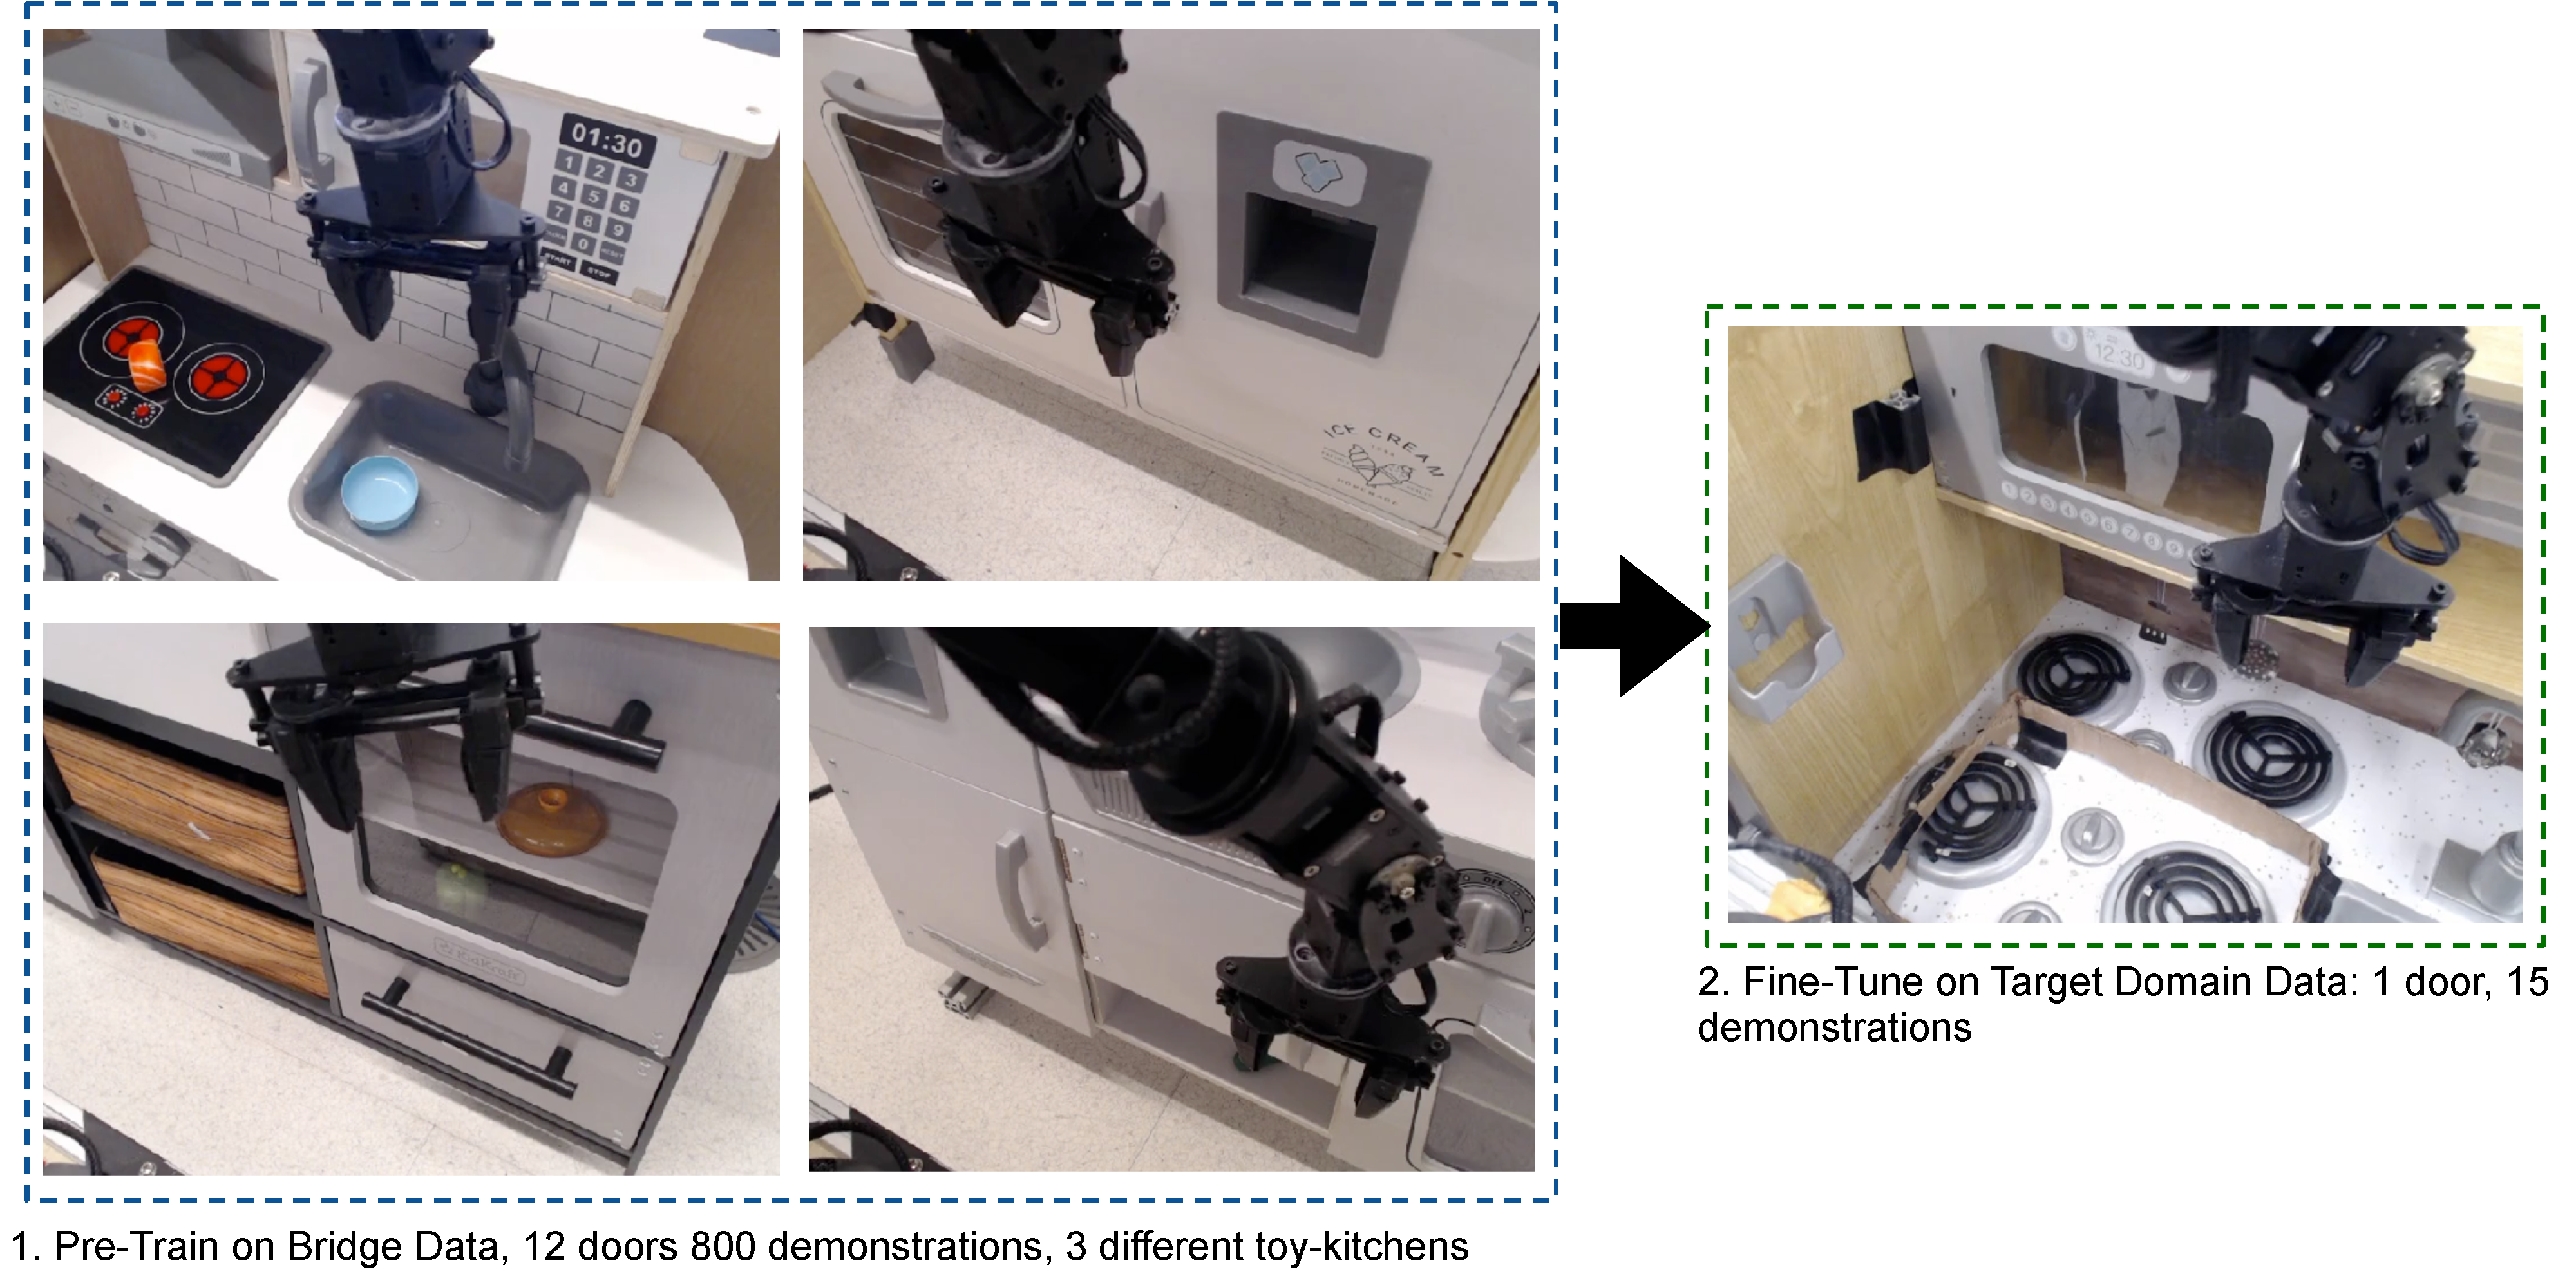
\includegraphics[width=0.83\linewidth]{scenario2_overview.pdf}
  \caption{\footnotesize \textbf{Illustration of pre-training data and fine-tuning data used for Scenario 2 (door opening)}: transferring a behavior to a held-out domain.}
  \vspace{-0.5cm}
  \label{fig:door_open_setup}
\end{figure}


\textbf{Pre-training data.} The pre-training data in Scenario 2 consists of 800 door-opening demonstrations on 12 different doors across 3 different toykitchen domains.

\textbf{Target task and data.} The target task requires opening the door of an unseen microwave in toykitchen 1 using a target dataset of only 15 demonstrations.

\textbf{Quantitative evaluation protocol.} We run 20 rollouts with each method, counting successes when the robot opened the door by at least 45 degrees. To perform this successfully, there is a degree of complexity as the robot has to initially open the door till it's open to about 30 degrees. Then due to physical constraints, the robot needs to wrap around the door and push it open from the inside. To begin an evaluation rollout, we reset the robot to randomly sampled poses obtained from held-out demonstrations on the target door.  This is a compound task requiring the robot to first grab the door by the handle, next move around the door, and finally push the door open. As before, we match the initial pose of the robot as closely as possible for all the methods. 


\subsubsection{Scenario 3: Learning to Solve New Tasks in New Domains}

\begin{figure}
\centering
  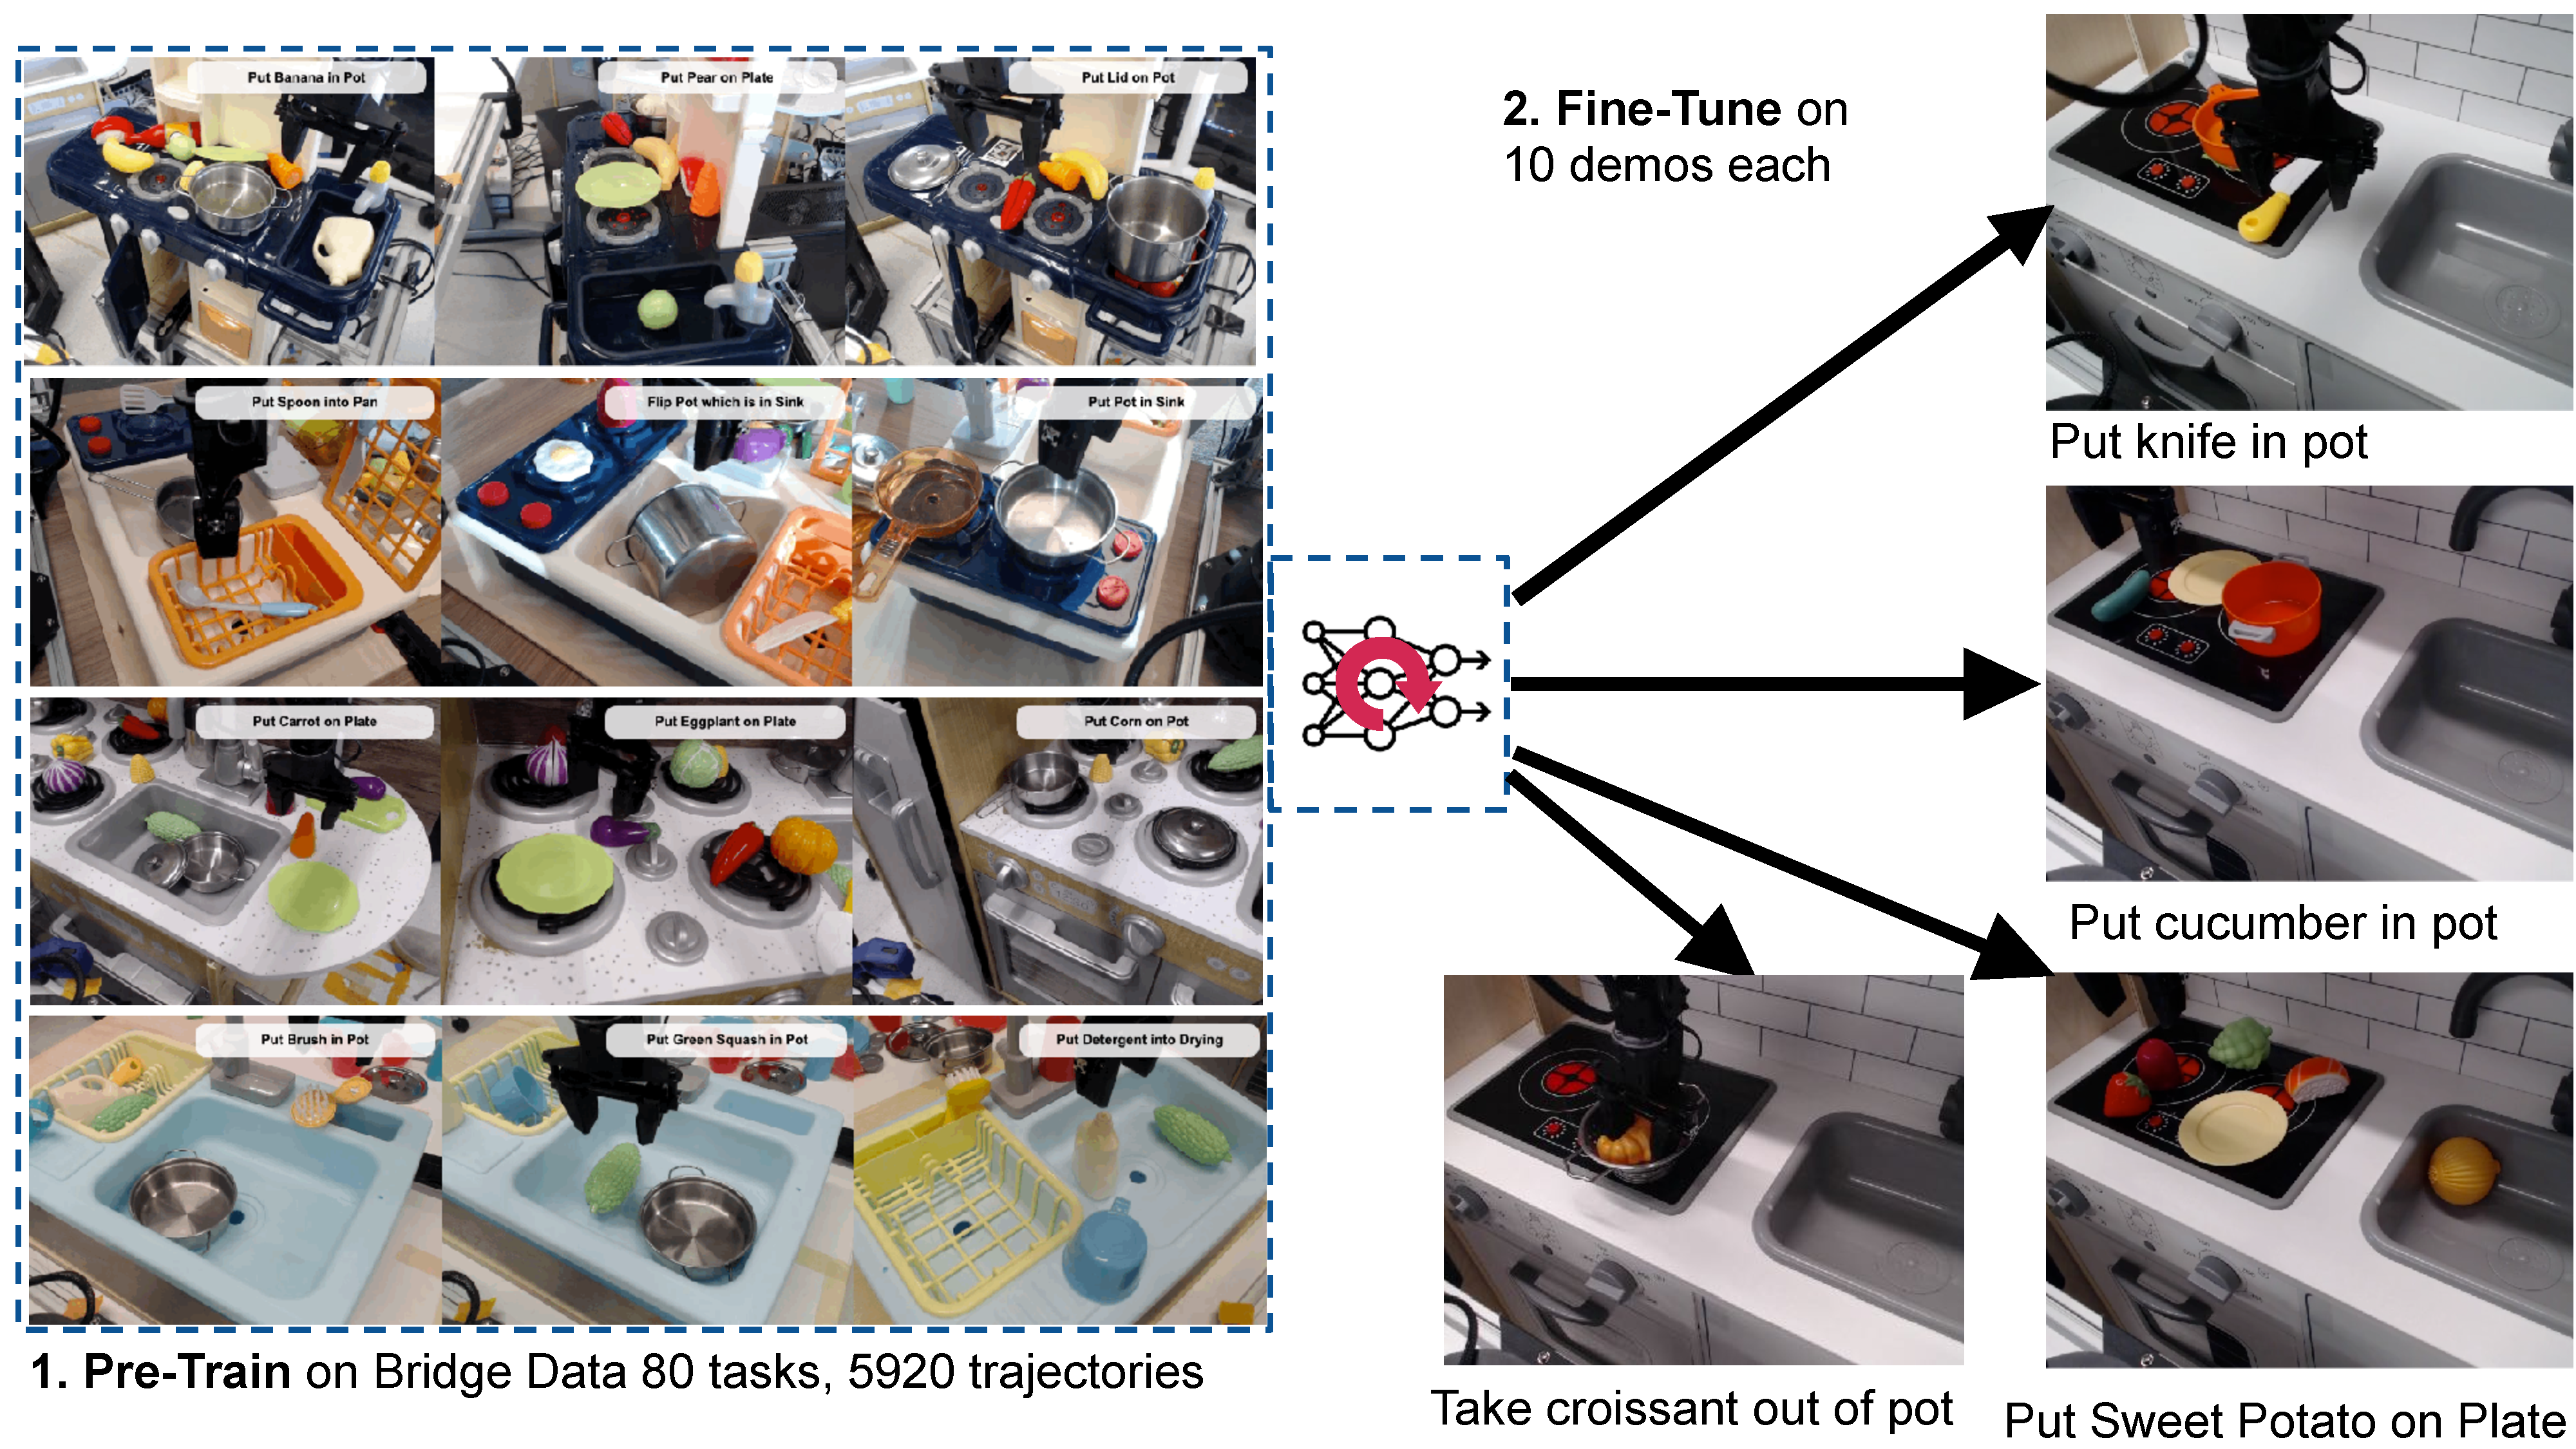
\includegraphics[width=0.83\linewidth]{scenario3_overview.pdf}
  \caption{\footnotesize {\textbf{Illustration of pre-training data and fine-tuning data used for the new tasks we have added in Scenario 3}. The goal is to learn to solve new tasks in new domains starting from the same pre-trained initialization and when fine-tuning is only performed using 10-20 demonstrations of the target task.}}
  \label{fig:scenario4_overview}
\end{figure}

\textbf{Pre-training data.} All pick-and-place data in the bridge dataset~\citep{ebert2021bridge} except any demonstration data collected in toykitchen~6, where our evaluations are performed.

\textbf{Target task and data.} The target task requires placing corn in a pot in the sink in the new target domain and the target dataset provides 10 demonstrations for this task. These target demonstrations are sampled from the bridge dataset itself.

\textbf{Quantitative evaluation protocol.} During the evaluation we were unable to exactly match the camera orientation used to collect the target demonstration trajectories, and therefore ran evaluations with a slightly modified camera view. This presents an additional challenge for any method as it must now generalize to a modified camera view of the target toykitchen domain, without having ever observed this domain or this camera view during training. We sampled initial poses for our method by choosing transitions from a held-out dataset of demonstrations of the target task and resetting the robot to those initial poses for each method. We attempted to match the positions of objects across methods as closely as possible.

\subsubsection{More Tasks in Scenario 3: Learning to Solve Multiple New Tasks in New Domains From the Same Initialization}
\label{app:scenario4}

In Appendix~\ref{app:exp_results}, we have now added results for more tasks in Scenario 3. The details of these tasks are as follows:

\textbf{Pre-training data.} All pick-and-place data from bridge dataset~\citep{ebert2021bridge} except data from toykitchen~6.

\textbf{Target task and data.} We consider four downstream tasks: take croissant from a metallic bowl, put sweet potato on a plate, place the knife in a pot, and put cucumber in a bowl. We collected 10 target demonstrations for the croissant, sweet potato, and put cucumber in bowl tasks, and 20 target demonstrations for the knife in pot task. A picture of these target tasks is shown in Figure \ref{fig:scenario4_overview}.

\textbf{Qualitative evaluation protocol.} For our evaluations, we utilize either 10 or 20 evaluation rollouts. As with all of our other quantitative results, we evaluate all the baseline approaches and \methodname starting from an identical set of initial poses for the robot. These initial poses are randomly sampled from the poses that appear in the first 10 timesteps of the held-out demonstration trajectories for this target task. For the configuration of objects, we test our policies in a variety of task-specific configurations that we discuss below:

\begin{itemize}
    \item \textbf{Take croissant from metallic bowl:} For this task, we alternate between two kinds of positions for the metallic bowl. In the ``easy'' positions, the metallic bowl is placed roughly vertically beneath the robot's initial starting pose, whereas in the ``hard'' positions, the robot must first move itself to the right location of the bowl and then execute the policy.
    \item \textbf{Put the cucumber in bowl:} We run 10 evaluation rollouts starting from 10 randomly sampled initial poses of the robot for our evaluations. Here we moved the bowl between the two stovetops in each trial. 
    \item \textbf{Put sweet potato on plate:} For this task, we performed 20 evaluation rollouts. We only sampled 10 initial poses for the robot, but for each position, we evaluated every policy on two orientations of the sweet potato (i.e., the sweet potato is placed on the table on its flat face or on its curved face). Each of these orientations presents some unique challenges, and evaluating both of them allows us to gauge how robust the learned policy is to changes in orientation. The demonstration data had a variety of orientations for the sweet potato object that differed for each collected trajectory. 
    \item \textbf{Place knife in pot:} We evaluate this task over 10 evaluation rollouts, where the first five rollouts use a smaller knife, while the other five rollouts use a larger knife (shown in Figure~\ref{fig:setup_overview}). Each knife was seen in the demonstration dataset with equal probability.
\end{itemize}

We will discuss the results obtained on these new tasks in Appendix~\ref{app:exp_results}.


\subsection{Additional Experimental Results}
\label{app:exp_results}

\begin{figure}[h]
\vspace{-0.3cm}
\centering
  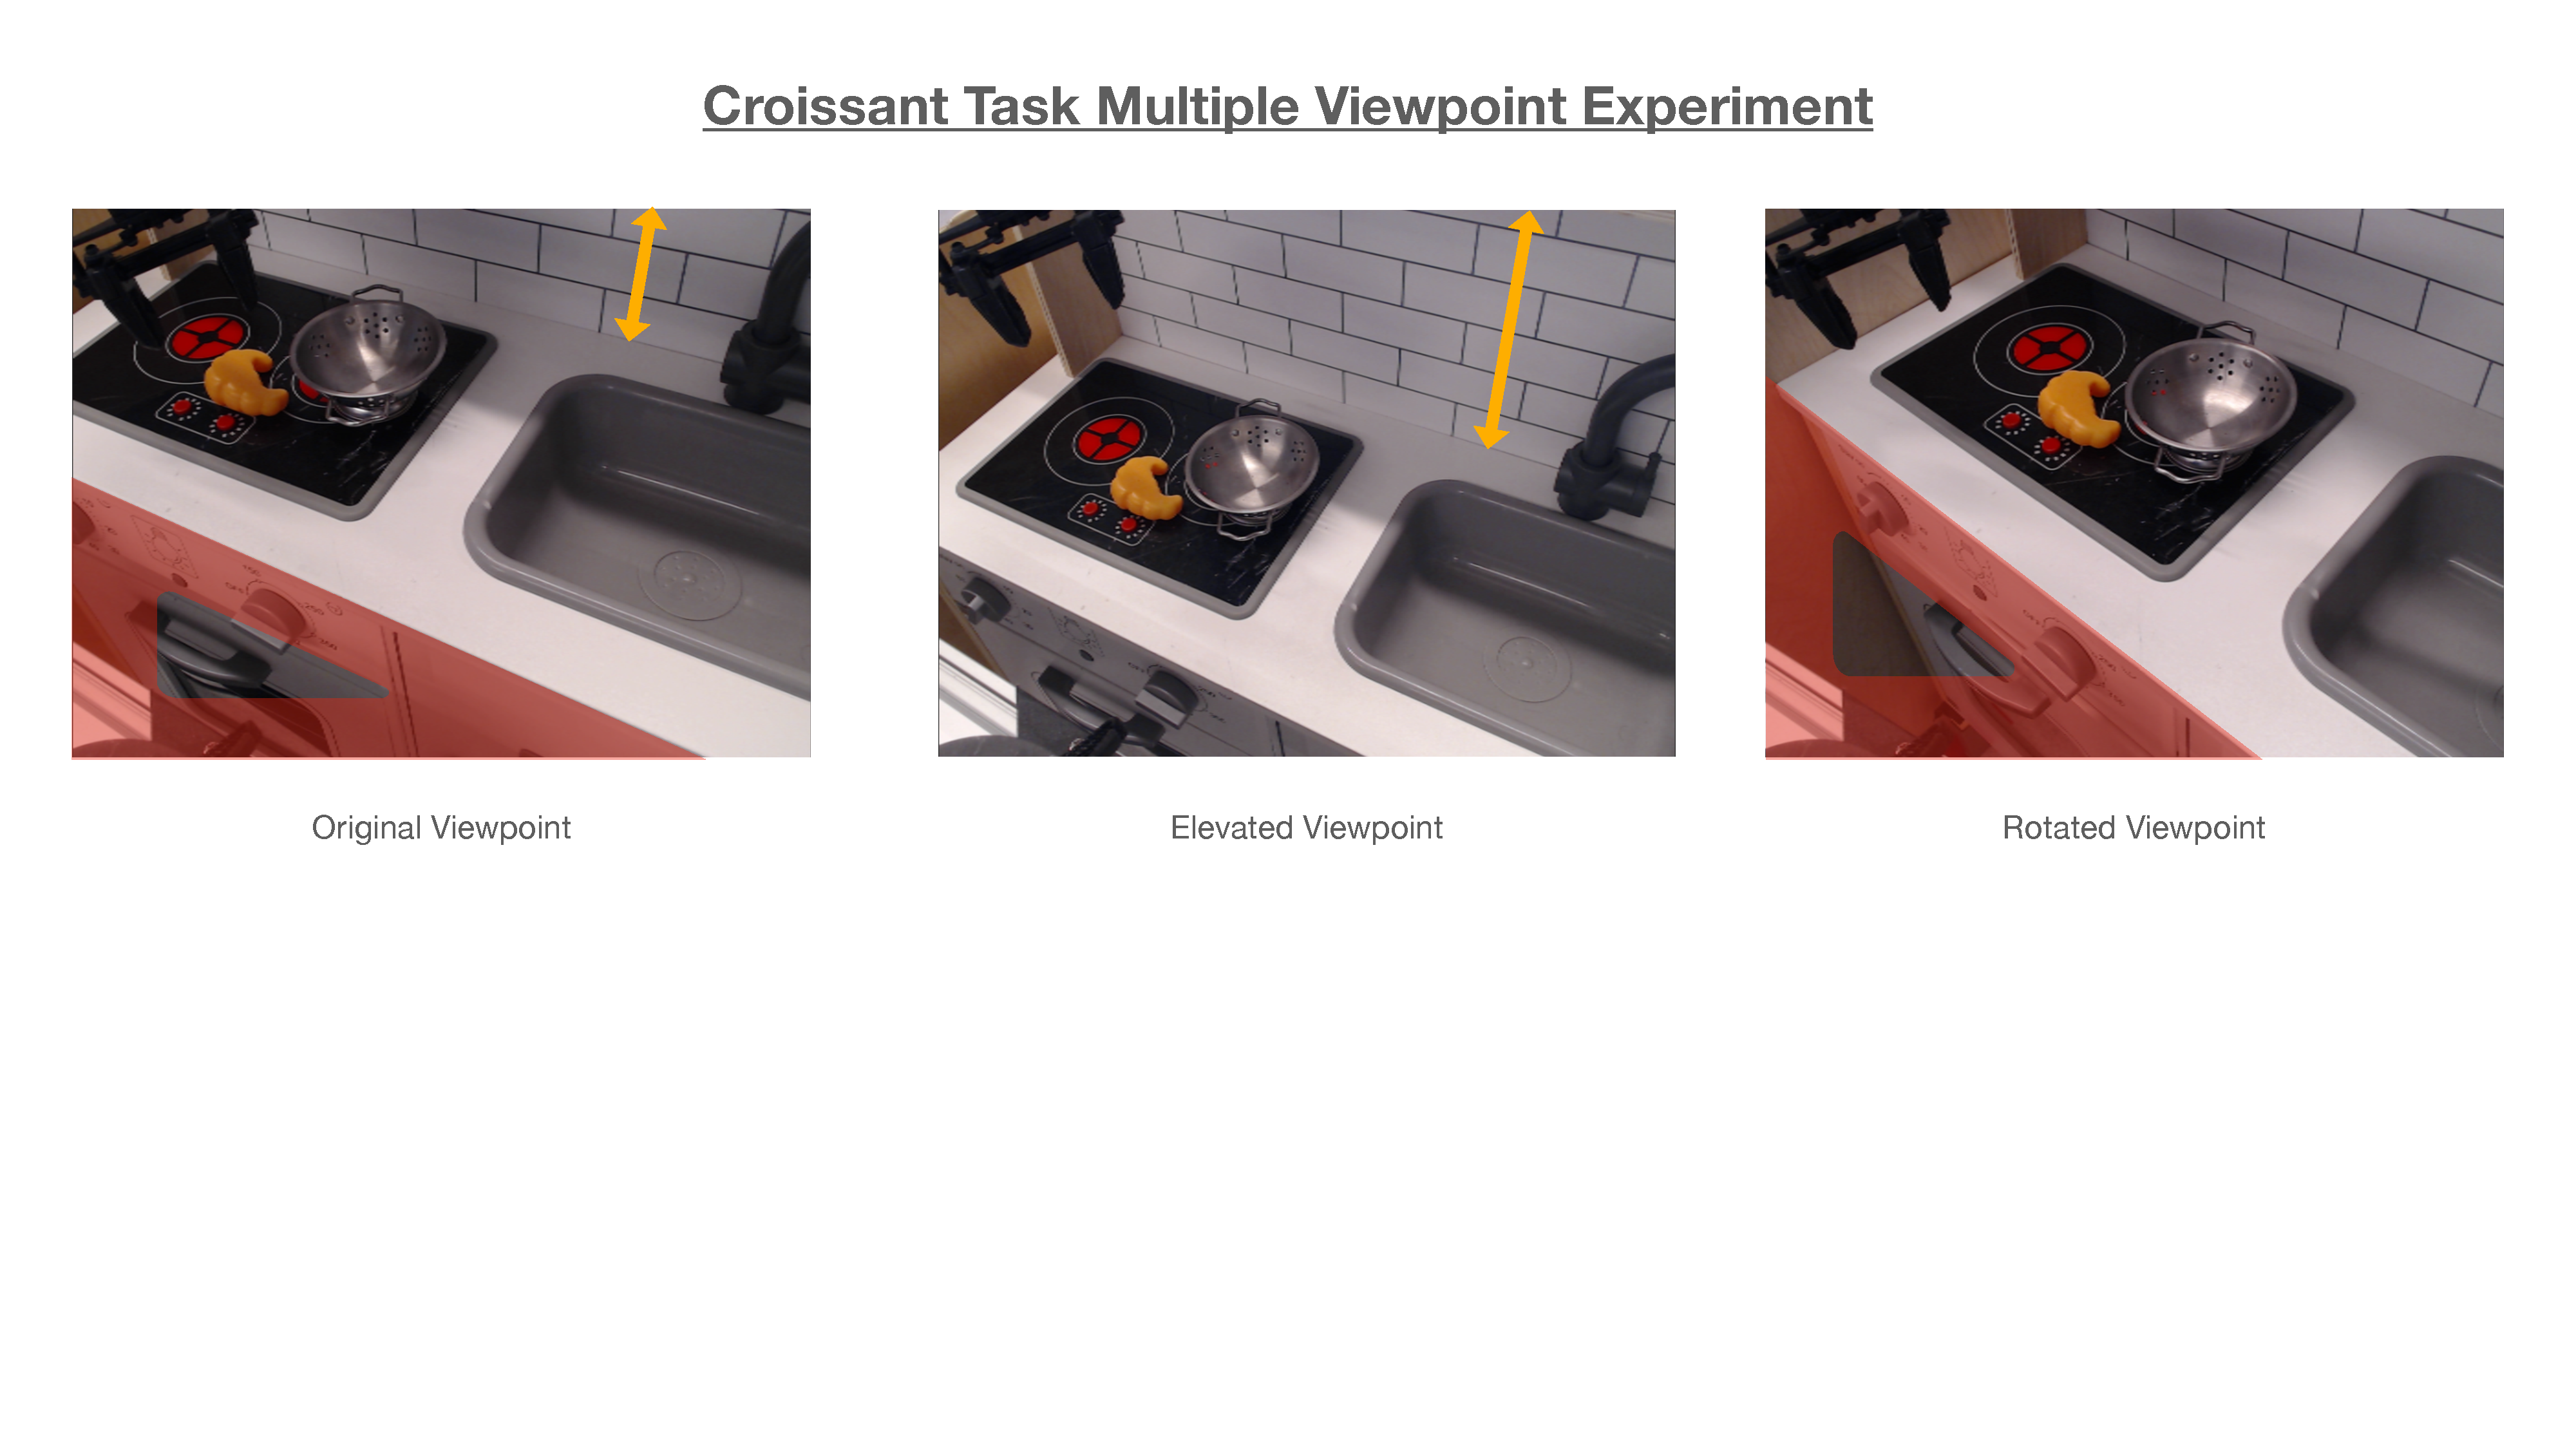
\includegraphics[width=0.9\linewidth]{MultViewpoint.pdf}
  \vspace{-0.3cm}
  \caption{\footnotesize \textbf{Sample observations from different camera viewpoints, only used during fine-tuning}. \textbf{Left:} the original camera viewpoint found in Figure~\ref{fig:scenario4_overview}. \textbf{Middle:} an elevated camera viewpoint where the robot and camera have been raised 7 cm. \textbf{Right:} a rotated camera viewpoint where the kitchen has been slightly translated and rotated 15 degrees counterclockwise relative to the camera and robot.}
  \label{fig:multviewpoint}
  \vspace{-0.2cm}
\end{figure}

\textbf{Finetuning to novel camera viewpoints:} Even though Scenario 3 already presents a novel toy-kitchen domain and previously unseen objects during finetuning, we also evaluate \methodname on a more challenging scenario where we additionally alter the camera viewpoint during finetuning. We apply two kinds of alterations to the camera: \textbf{(a)} we elevate the mounting platform of the camera by 7 cm, which necessitates adapting the way the physical coordinates of the robot end-effector are interpreted by the policy, and \textbf{(b)} we rotate the camera by about 15 degrees to induce a more oblique image observation than what was ever seen during pre-training. Note that in both of these scenarios, the robot has never encountered such camera viewpoints during pre-training, which makes this scenario even more challenging. The original dataset in \citep{ebert2021bridge} had the camera elevated to the same position for each domain and always ensured the kitchen was parallel to the camera platform, with translations being the primary changes in the scene for each domain. In Table \ref{tab:viewpoint_comp}, we present our results comparing \methodname and BC (finetune). Observe that \methodname still clearly outperforms BC (finetune), and attains performance close to that of \methodname in Table~\ref{tab:scenario4}, indicating that such shifts in the camera do not drastically hurt \methodname.


\begin{table}[h]
% \small{
\centering
\begin{tabular}{l|r|r}
\toprule
\textbf{Method} & \textbf{Elevated Viewpoint} & \textbf{Rotated Viewpoint}  \\ \midrule
BC (finetune) & 2/10  & 3/10  \\
\textbf{\methodname (Ours)} & \textbf{6/10}  & \textbf{7/10}  \\
\bottomrule
\end{tabular}
\vspace{-0.1cm}
\caption{\footnotesize{\textbf{Comparison of \methodname and BC (finetune), when evaluated on novel camera viewpoints} with elevated and rotated cameras as shown in Figure~\ref{fig:multviewpoint} for the croissant task. Observe that \methodname still outperforms BC (finetune) in this setting and attains more than 2x success rate of BC (finetune).}}
\label{tab:viewpoint_comp}
\end{table}

\subsubsection{Expanded Discussion: Why Does \methodname Outperform BC-based methods, Even With Demonstration Data?}

One natural question to ask given the results in this paper is: why does utilizing an offline RL method for pre-training and finetuning as in \methodname outperform BC-based methods even though the dataset is quite ``BC-friendly'', consisting of only demonstrations? One might speculate that an answer to this question is that our BC baseline can be tuned to be much better. However, note that our BC baseline is not suboptimally tuned. We utilize the procedure prescribed by prior work~\citep{ebert2021bridge} for tuning BC as we discuss in Appendix~\ref{app:hyperparams}. In addition, the fact that \textbf{BC (joint)} does actually outperform \textbf{CQL (joint)} in many of our experiments, indicates that our BC baselines are well-tuned. To explain the contrast to \citet{ebert2021bridge}, note that the setup in this prior work utilized many more target task demonstrations ($\geq 50$ demonstrations from the target task) compared to our evaluations, which might explain why our BC-baseline numbers are lower in an absolute sense. Therefore, the technical question still remains: why  would we expect \methodname to perform better than BC? We will attempt to answer this question using some empirical evidence and visualizations. Also, we will aim to provide intuition for why our approach \methodname outperforms the baseline.

\begin{figure}[h]
\centering
\vspace{-0.4cm}
  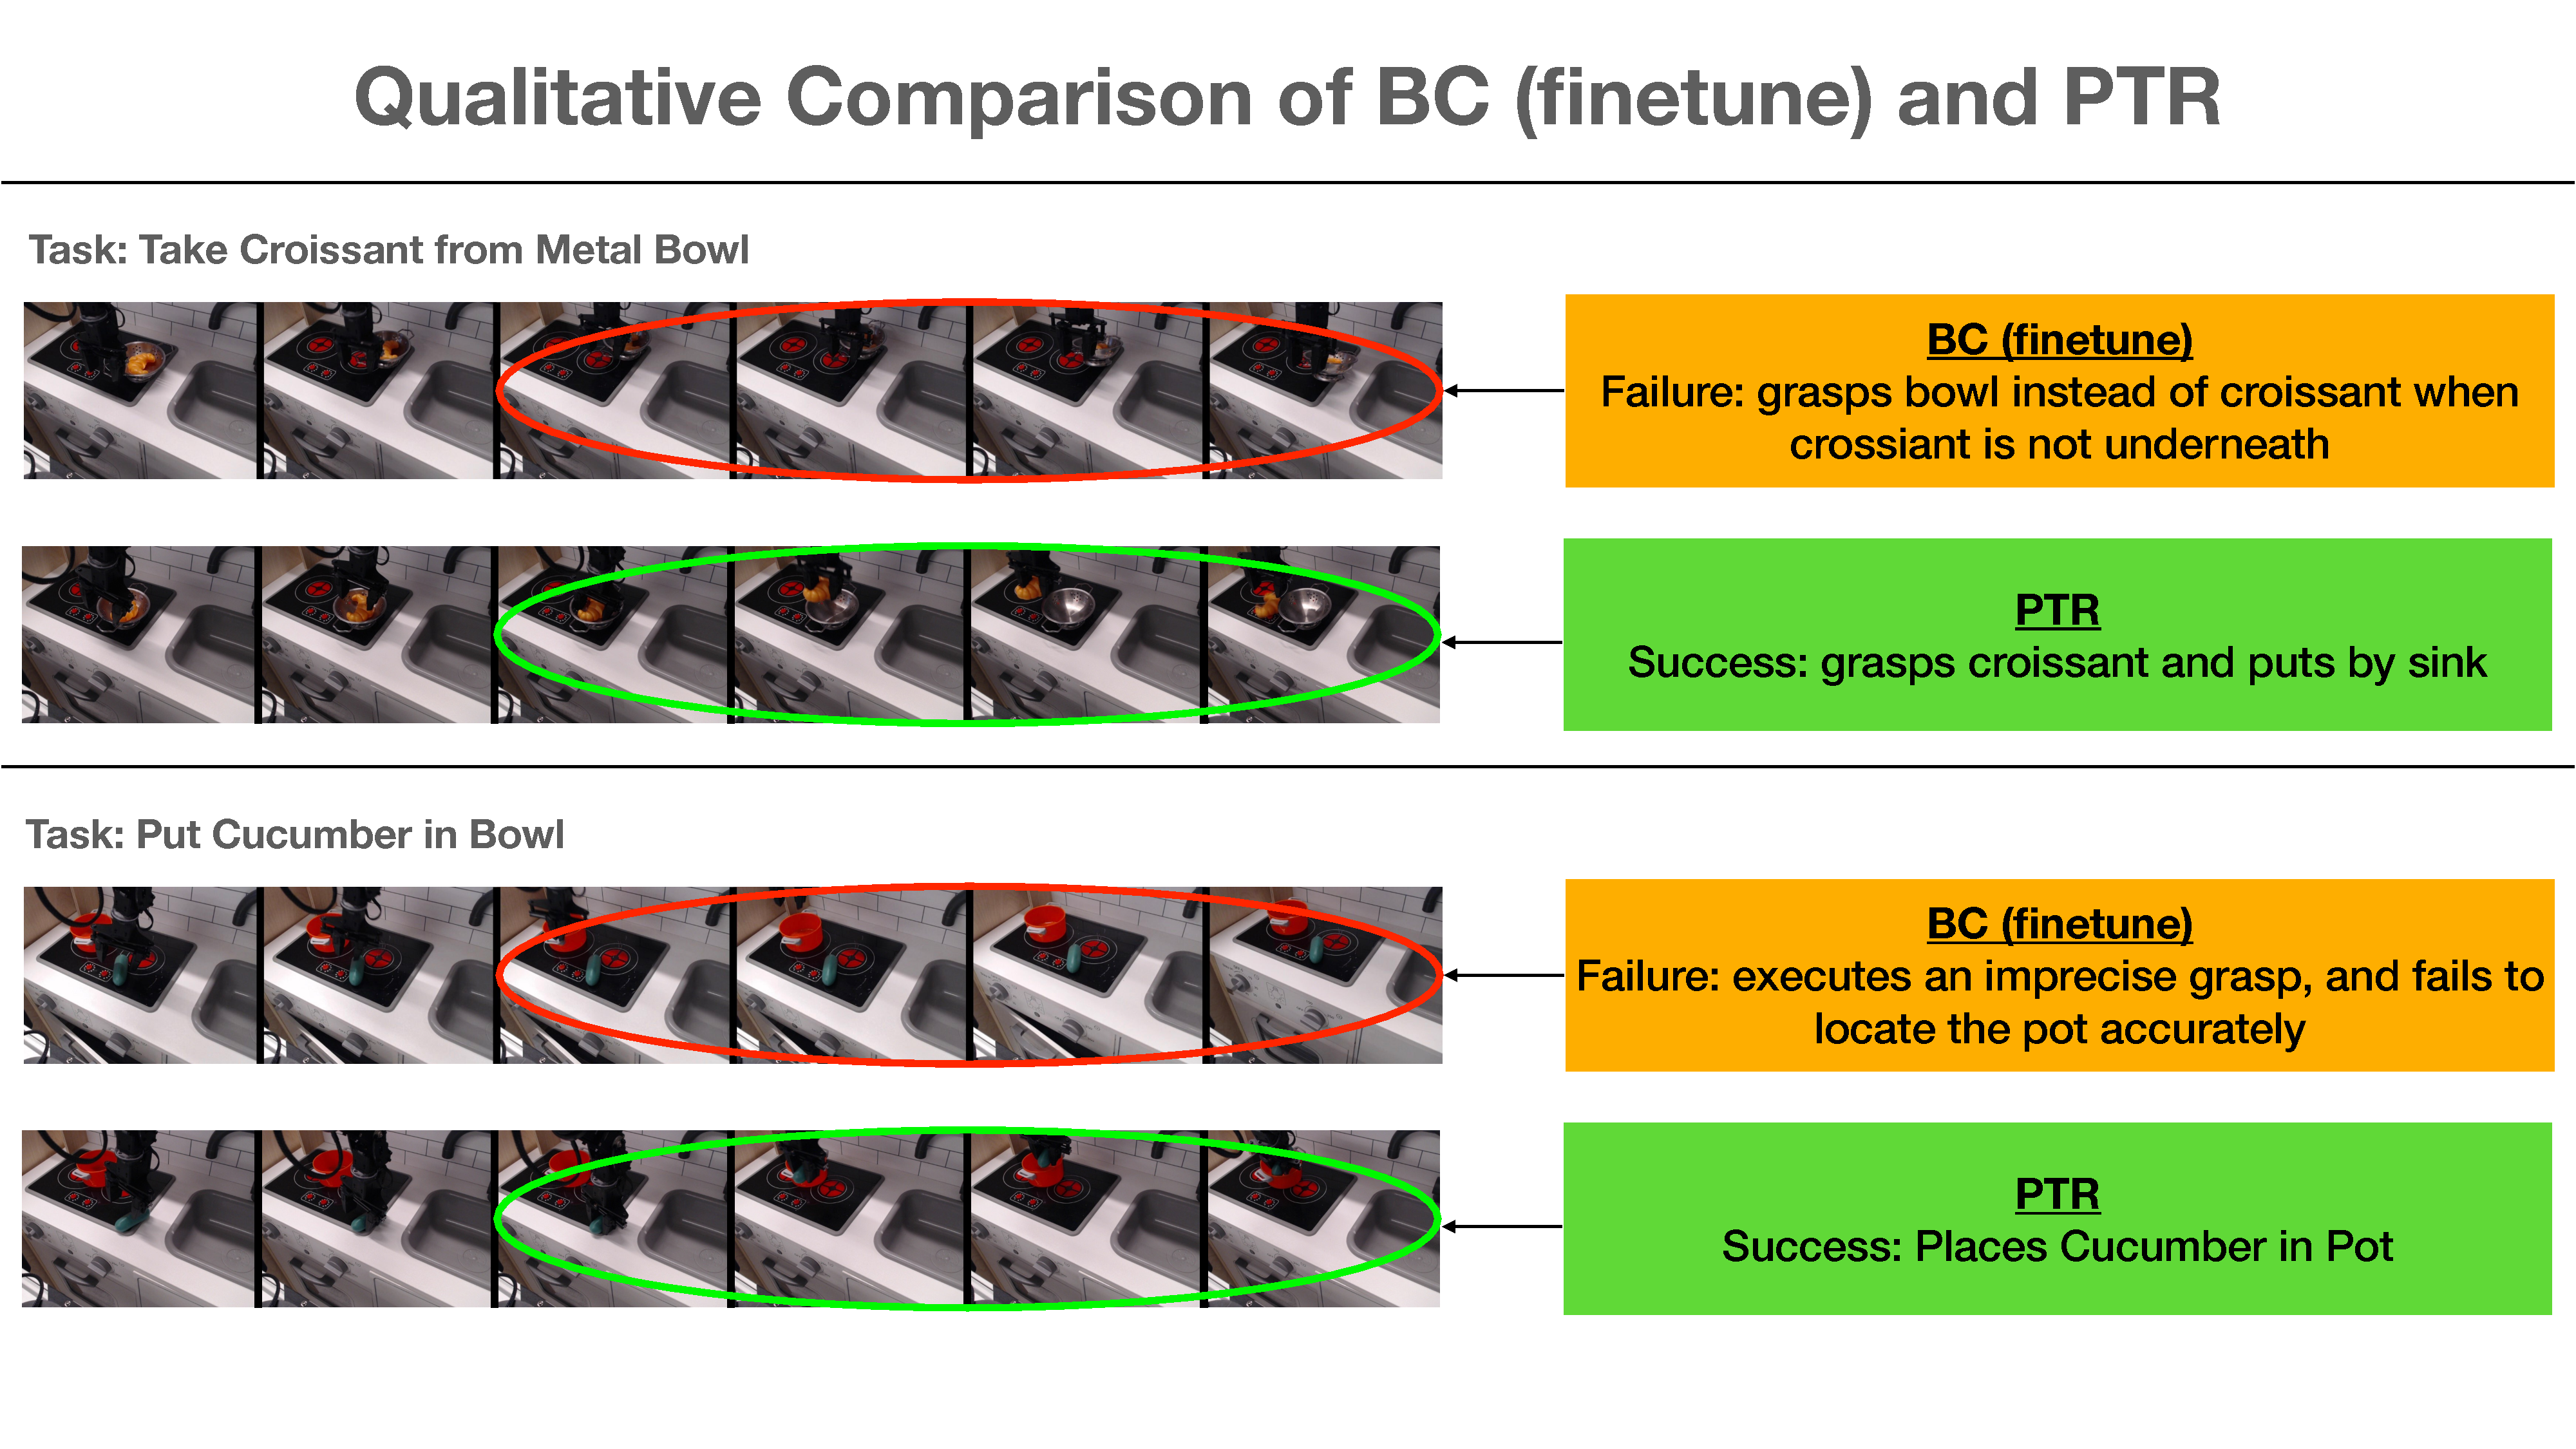
\includegraphics[width=0.83\linewidth]{Comparison.pdf}
  \vspace{-0.5cm}
  \caption{\footnotesize \textbf{Qualitative successes of \methodname visualized alongside failures of BC (finetune).} As an example, observe that while \methodname is accurately able to reach to the croissant and grasp it to solve the task, BC (finetune) is imprecise and grasps the bowl instead of the croissant resulting in failure.}
  \label{fig:dumb_behavior2}
  \vspace{-0.3cm}
\end{figure}


\textbf{To begin answering this question,} it is instructive to visualize some failures for a BC-based method and qualitatively attempt to understand why BC is worse than utilizing \methodname. We visualize some evaluation rollouts for \textbf{BC (finetune)} and \methodname as film strips in {Figure~\ref{fig:dumb_behavior2}}. Specifically, we visualize evaluation rollouts that present a challenging initial state. For example, for the rollout from the take croissant out of metallic pot task, the robot must first accurately position itself over the croissant before executing the grasping action. Similarly, for the rollout from the cucumber task, the robot must accurately locate the bowl and precisely try to grasp the cucumber. Observe in {Figure~\ref{fig:dumb_behavior}} that \textbf{BC (finetune)} typically fails to accurately reach the objects of interest (croissant and the bowl) and executes the grasping action prematurely. On the other hand, \methodname is more robust in these situations and is able to accurately reach the object of interest before it executes the grasping action or the releasing action. Why does this happen?  

\textbf{To understand why this happens}, one mental model is to appeal to the critical states argument from \citet{kumar2022should}. Intuitively, this argument suggests that in tasks where the robot must precisely accomplish actions at only a few specific states (called ``\textbf{critical states}'') to succeed, but the actions at other states (called ``non-critical states'') do not matter as much. Thus, offline RL-style methods can outperform BC-based methods even with demonstration data. This is because learning a value function can enable the robot to reason about which states are more important than others, and the resulting policy optimization can ``focus'' on taking correct actions at such critical states. Our real-world evaluation scenarios exhibit such a structure. The majority of the actions that the robot must take to reach the object do not need to be precise as long as they generally move the robot in the right direction. However, in order to succeed, the robot must critically ensure to position the arm is right above the object in a correct orientation and position itself right above the container in which the object must be placed. These are the critical states and special care must be taken to execute the right action in these states. In such scenarios, the argument of \citet{kumar2022should} would suggest that offline RL should be better. We believe that we observe a similar effect in our experiments: the learned BC policies are often not precise-enough at those critical states where taking the right action is critical to success.  

\begin{figure}[h]
\centering
\vspace{-0.4cm}
  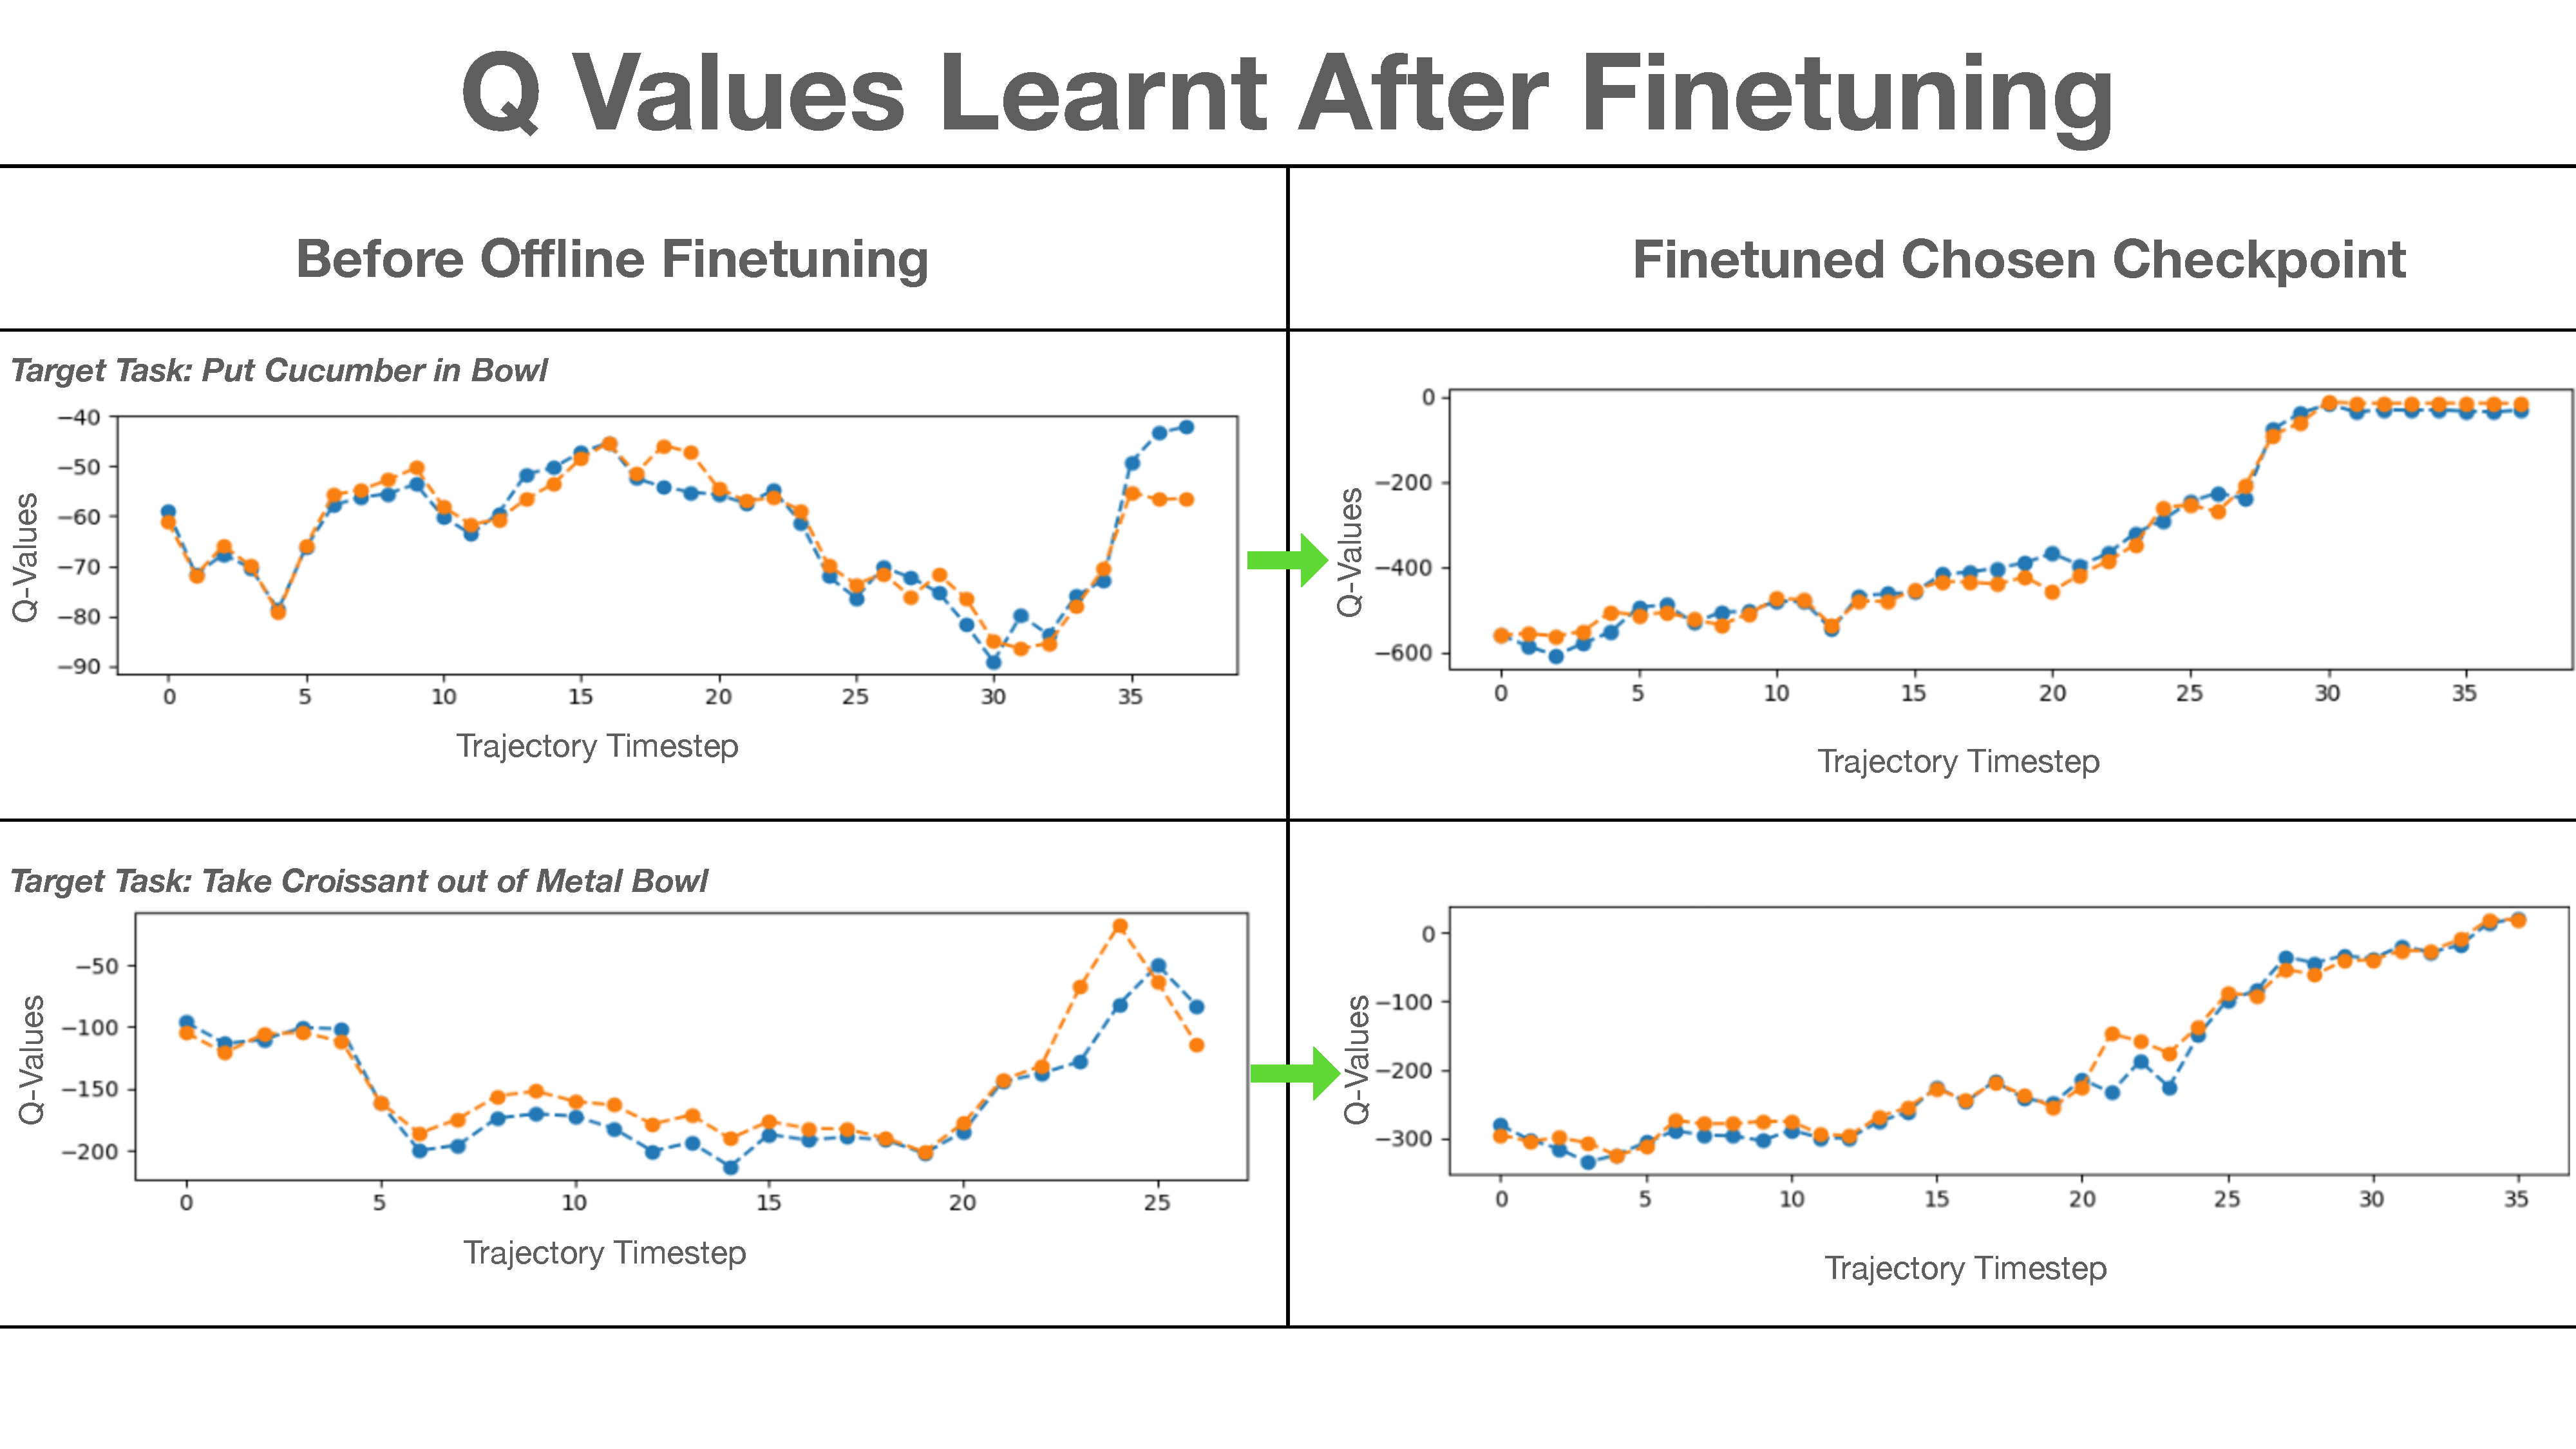
\includegraphics[width=0.78\linewidth]{FinetuningQvalPlot.pdf}
  \vspace{-0.5cm}
  \caption{\footnotesize \textbf{Evolution of Q-values on the target task} over the process of fine-tuning with \methodname. Observe that while the learned Q-values on \emph{held-out} trajectories from the dataset just at the beginning of Phase 2 (finetuning) do not exhibit a roughly increasing trend, the checkpoint of \methodname we choose to evaluate exhibits a generally increasing trend in the Q-values despite having access to only 10 demonstrations for these target tasks.}
  \label{fig:finetunedQvals2}
  \vspace{-0.3cm}
\end{figure}

{As supporting evidence} to the discussion above, we further visualize the Q-values over held-out trajectories from the target demonstration data that were never seen by \methodname during fine-tuning in {Figure~\ref{fig:finetunedQvals2}}. To demonstrate the contrast, we present the trend in Q-values before fine-tuning and for the checkpoint selected for evaluation after fine-tuning on the target task. Observe that the Q-values for the chosen checkpoint generally increase over the course of the trajectory indicating that the learned Q-function is able to fit well with the target data. Also, the learned Q-function generalizes to held-out trajectories despite the fact that only 10 demonstrations were provided during the fine-tuning phase. This evidence supports the claim that it is reasonable to expect the learned Q-function to be able to focus on the more critical decisions in the trajectory.

\textbf{To further support our hypothesis that \methodname outperforms BC-based methods because the learned value function enables us to learn about ``critical'' decisions}, we run an experiment that essentially runs a weighted version of BC during finetuning, where the weights are provided by exponentiated advantage values, where the advantages are defined as $A_\theta(\bs, \ba) = Q_\theta(\bs, \ba) - \max_{\ba'} Q_\theta(\bs, \ba')$ under a Q-function learned by \methodname. This approaches essentially matches BC finetuning in all aspects: the policy parameterization, the loss function (mean-squared error), and the details of the training are kept identical to our BC baselines, with the exception of an additional weight given by $\exp(A_\theta(\bs, \ba))$ on a given transition $(\bs, \ba, r, \bs')$ observed in the set of limited task-specific demonstrations. We refer to this approach as ``advantage-weighted BC finetuning''.

In contrast to our BC (finetune) results from Table~\ref{tab:scenario4}, where \methodname significantly outperformed BC (finetune), observe in Table~\ref{tab:aw_bc}, that advantage-weighted BC (finetune) performs comparably to \methodname on the two tasks we studied for our analysis. This result is significant since it implies that all other factors kept identical, utilizing the weights given by the Q-function is the crucial factor in improving the performance of BC and avoids the qualitative failure modes associated with BC methods shown in Figure~\ref{fig:dumb_behavior2}.

\begin{table}[h]
% \small{
\centering
\resizebox{0.99\linewidth}{!}{\begin{tabular}{c|r|r||r}
\toprule
\textbf{Task} & \textbf{BC (finetune)} & \textbf{\methodname (Ours)} &\textbf{Advantage-weighted BC (finetune)}  \\ \midrule
Put cucumber in pot &  0/10 & 5/10 &  {5/10} \\
Take croissant from metal bowl & 3/10 &  7/10  & {6/10} \\
\bottomrule
\end{tabular}}
\vspace{0.1cm}
\caption{\footnotesize{\textbf{Performance of advantage-weighted BC} on two tasks from Table~\ref{tab:scenario4}. Observe that weighting the BC objective using advantage-weights computed using the Q-function learned by \methodname leads to much better performance than standard BC (finetune), and close to PTR. This test indicates that the Q-function in \methodname allows us to focus on more critical points, thereby preventing the failures discussed in Figure~\ref{fig:dumb_behavior2}.}}
\label{tab:aw_bc}
\end{table}


\subsubsection{Hyperparameters for \methodname and Baseline Methods}
\label{app:hyperparams}

In this section, we will present the hyperparameters we use in our experiments and explain how we tune the other hyperparameters for both our method \methodname and the baselines we consider.  

\textbf{\methodname.} Since \methodname utilizes CQL as the base offline RL method, it trains two Q-functions and a separate policy, and maintains a delayed copy of the two Q-functions, commonly referred to as target Q-functions. We utilize completely independent networks to represent each of these five models (2 Q-functions, 2 target Q-functions, and the policy). We also do not share the convolutional encoders among them. As discussed in the main text, we rescaled the action space to $[-1, 1]^{|\mathcal{A}|}$ to match the one used by actor-critic algorithms, and utilized a Tanh squashing function at the end of the policy. We used a CQL $\alpha$ value of 10.0 for our pick-and-place experiments. The rest of the hyperparameters for training the Q-function, the target network updates, and the policy are taken from the standard training for image-based CQL from \citet{singh2020cog} and are presented in Table~\ref{tab:hparams_cql} below for completeness. The hyperparameters we choose are essentially the network design decisions of \textbf{(1)} utilizing group normalization instead of batch normalization, \textbf{(2)} utilizing learned spatial embeddings instead of standard mean pooling, \textbf{(3)} passing in actions at each of the fully connected layers of the Q-network and the hyperparameter $\alpha$ in CQL that must be adjusted since our data consists of demonstrations. We will ablate the new design decisions explicitly in Appendix~\ref{app:design}.

\begin{table*}[h]
% \small{
\centering
\begin{tabular}{l|c}
\toprule
\textbf{Hyperparameter} & \textbf{Value}\\  \midrule
Q-function learning rate & 3e-4 \\
Policy learning rate & 1e-4 \\
Target update rate & 0.005 (soft update with Polyak averaging) \\
Optimizer type & Adam \\
Discount factor $\gamma$ & 0.96 (since trajectories have a length of only about 30-40) \\
Use terminals & True \\
Reward shift and scale & shift = -1, scale = 10.0 \\
CQL $\alpha$ & 10.0 \\
Use Color Jitter & True \\
Use Random Cropping & True \\
\bottomrule
\end{tabular}
\vspace{0.07cm}
\caption{\footnotesize{\textbf{Main hyperparameters for CQL training in our real-world experiments.} In the simulation, we utilize a smaller $\alpha$ for CQL, $\alpha=1.0$, and a larger discount $\gamma = 0.98$ since trajectories in the simulation are about 60-70 timesteps in length. }}
\label{tab:hparams_cql}
% \vspace{-0.5cm}
\end{table*}

The only other hyperparameter used by \methodname is the mixing ratio $\tau$ that determines the proportion of samples drawn from the pre-training dataset and the target dataset during the offline finetuning phase in \methodname. We utilize $\tau = 0.7$ for our experiments with \methodname in the main paper, and use $\tau = 0.9$ for the additional experiments we added in the Appendix. This is because $\tau=0.9$ (more bridge data, and a smaller amount of target data) was helpful in scenarios with very limited target data.  

In order to perform checkpoint selection for \methodname, we utilized the trends in the learned Q-values over a set of held-out trajectories on the target data as discussed in Section~\ref{sec:design_choices}. We did not tune any other algorithmic hyperparameters for CQL, as these were taken directly from \citep{singh2020cog}.  

\textbf{BC (finetune).}
We trained BC in a similar manner as \citet{ebert2021bridge}, utilizing the design decisions that this prior work found optimal for their experiments. The policy for BC utilizes the very same ResNet 34 backbone as our RL policy since a backbone based on ResNet 34 was found to be quite effective in \citet{ebert2021bridge}. Following the recommendations of \citet{ebert2021bridge} and based on result trends from our own preliminary experiments, we chose to not utilize the tanh squashing function at the end of the policy for any BC-based method, but trained a deterministic BC policy that was trained to regress to the action in the demonstration with a mean-squared error (MSE) objective. 

\begin{table}[h]
% \small{
\centering
\begin{tabular}{l|c}
\toprule
\textbf{Hyperparameter} & \textbf{Value}\\  \midrule
Policy learning rate & 1e-4 \\
Optimizer type & Adam \\
Use Color Jitter & True \\
Use Random Cropping & True \\
Dropout & 0.4 \\
\bottomrule
\end{tabular}
\vspace{0.07cm}
\caption{\footnotesize{\textbf{Main hyperparameters for Behavior Cloning Baseline Training in our real-world and simulation experiments.} Note: architecture design choices follow closely to \methodname design choices.}}
\label{tab:hparams_cql}
\vspace{-0.4cm}
\end{table}

In order to perform cross-validation, checkpoint, and model selection for our BC policies, we follow guidelines from prior work~\citep{ebert2021bridge,emmons2021rvs} and track the MSE on a held-out validation dataset similar to standard supervised learning. We found that a ResNet 34 BC policy attained the smallest validation MSEs in general, and for our evaluations, we utilized a checkpoint of a ResNet 34 BC policy that attained the smallest MSE.   

Analogous to the case of \methodname discussed above, we also ablated the performance of BC for a set of varying values of the mixing ratio $\tau$, but found that a large value of $\tau = 0.9$ was the most effective for BC, and hence utilized $\tau = 0.9$ for BC (finetune) and BC (joint).

\textbf{BC (joint) and CQL (joint).} The primary distinction between training \textbf{BC (joint)} and \textbf{BC (finetune)} and correspondingly, \textbf{CQL (joint)} and \methodname was that in the case of joint training, the target dataset was introduced right at the beginning of Phase 1 (pre-training phase), and we mixed the target data with the pre-training data using the same value of the mixing ratio $\tau$ used in for our fine-tuning experiments to ensure a fair comparison.

{
\textbf{Few-shot offline meta-RL (MACAW)~\citep{2020arXiv200806043M}:} We compare to two variants of this algorithm and perform an \textbf{extensive} sweep over several hyperparameters, shown in Table~\ref{tab:hparams_macaw}. 
}

{
We trained two different variants of MACAW in our evaluation: \textbf{(1)} Pre-training on the bridge data in Scenario 3 and then fine-tuning on target data of interest, and \textbf{(2)} adapting a set of existing task identifiers to the target task of interest utilizing the same pre-training and fine-tuning domains. We performed early stopping on the meta-training based on validation losses. From there, we started the meta-testing phase, adapting to the target domain of interest. Following \citet{2020arXiv200806043M}, we use a task mini-batch of 8 tasks at each step of optimization rather than using all of the training tasks. We clipped the advantage weight logits to the scale of 20 and attempted to utilize a policy network with a fixed and learned standard deviation. Additionally, we varied the number of Adaptation steps following prior work. Our evaluation protocol for MACAW entails utilizing the validation losses to choose an initial checkpoint for evaluation. Then, we consider checkpoints in the neighborhood ($\pm$ 50K gradient steps) to for evaluations as well and chose the max over all of these checkpoints as the final evaluation success rate.
}

{
Quantitatively, as seen in Table~\ref{tab:scenario4}, MACAW was unable to get non-zero success rates on any of the tasks we study. However, we did qualitatively observe nontrivial behavior seen in our evaluation rollouts. For instance, we found that the policies trained via MACAW could consistently grasp the object of interest but were unable to localize where to place the object correctly. Several trials involved hovering around with the object of interest and not placing the object in the container. Other trials involved the agent failing to grasp the object.
}

\begin{table}[h]
% \small{
\centering
\begin{tabular}{l|c}
\toprule
\textbf{Hyperparameter} & \textbf{Value}\\  \midrule
Optimizer & Adam \\
Outer Policy learning rate & 1e-4 \\
Outer Value learning rate & 1e-5, 1e-6 \\
Inner Policy learning rate & 1e-2, 1e-3 \\
Inner Value learning rate & 1e-3, 1e-4 \\
Auxilary Advantage Coefficient & 1e-2, 1e-3, 1e-4 \\
Policy Parameterization & Fixed std, Learned std \\
AWR Policy Temperature & 1, 10, 20 \\
Number of Adaptation Steps & 1, 2, 3 \\
Task Batch Size & 8 \\
Train Adaptation Batch Size & 64 \\
Eval Adaptation Batch Size & 64 \\
Max Advantage Clip & 20 \\
Use Color Jitter & True \\
Use Random Cropping & True \\

\bottomrule
\end{tabular}
\vspace{0.07cm}
\caption{{\footnotesize{\textbf{Main hyperparameters for Training MACAW~\citep{2020arXiv200806043M} in our real-world experiments.} Note: architecture design choices follow closely to \methodname design choices but hyperparameter design choices follow closely the suggestions in \citet{2020arXiv200806043M}.}}}
\label{tab:hparams_macaw}
\vspace{-0.2cm}
\end{table}

\textbf{Pre-trained R3M initialization~\citep{nair2022r3m}:} Next we compare \methodname to utilizing an off-the-shelf pre-trained representation given by R3M~\citep{nair2022r3m}. We compare two baselines that attempt to train an MLP policy on top of the R3M state representation by using BC (finetuning) and CQL (finetuning) respectively. To ensure that this baseline is well-tuned, we tried a variety of network sizes with 2, 3 or 4 MLP layers and also tuned the hidden dimension sizes in [256, 512, 1024]. We also utilized dropout as regularization to prevent overfitting and tuned a variety of values of dropout probability in [0, 0.1, 0.2, 0.4, 0.6, 0.8]. We observe in Table~\ref{tab:scenario4}, that on the four tasks we evaluate on, \methodname outperforms R3M, which indicates that training on the bridge dataset can indeed give rise to effective visual representations that are more suited to finetuning in our setting. The numbers we report in the table are the best over each parametric policy corresponding to each hyperparameter in our ablation. Checkpoint selection was done utilizing early stopping which is the last iteration where the validation error stops decreasing. Learning curves for this baseline can be found in our Anonymous Website.

\textbf{Pre-trained MAE initialization~\citep{he2111masked}:}
We took a similar training procedure to R3M for our MAE representation. We used an MAE trained on every image from the bridge dataset \citet{ebert2021bridge}. We then fine-tuned a specific target task with a similar ablation on network size, hidden dimension size, and regularization techniques such as dropout.  We observe in Table~\ref{tab:rep_learning_comparison}, that on the four tasks we evaluate on, \methodname outperforms R3M, which indicates that training on the bridge dataset can indeed give rise to effective visual representations that are more suited to finetuning in our setting. The numbers we report in the table are the best over each parametric policy corresponding to each hyperparameter in our ablation. Checkpoint selection was done utilizing early stopping which is the last iteration where the validation error stops decreasing. 

\textbf{Policy expressiveness study.}
We considered two policy expressiveness choices for BC to compare with our reference BC implementation that is implemented with a set of MLP layers. The first of the two choices was an \textbf{autoregressive policy} where the 7-dimensional action space was discretized into 100 bins. Each action was then predicted autoregressively conditioned on the observation, task id, and the action component from the previous dimension(s). The second approach was with the BeT Architecture from \citet{shafiullah2022behavior}. We utilized the reference implementation from the paper with the default suggested hyperparameters for this set of ablations. The window size for the MinGPT transformer was ablated over between 1, 2, and 10.

\subsection{Validating the Design Choices from Section~\ref{sec:design_choices} via Ablation Studies}
\label{app:design}

In this section, we will present ablation studies aimed to validate the design choices utilized by \methodname. We found these design choices quite crucial for attaining good performance. The concrete research questions we wish to answer are: \textbf{(1)} How important is utilizing a large network for attaining good performance with \methodname, and how does the performance of \methodname scale with the size of the Q-function?, \textbf{(2)} How effective is a learned spatial embedding compared to other approaches for aggregating spatial information? \textbf{(3)} Is concatenating actions at each fully-connected layer of the Q-function crucial for good performance?, \textbf{(4)} Is group normalization a good alternative to batch normalization? and \textbf{(5)} How does our choice of creating binary rewards for training affect the performance of \methodname?. We will answer these questions next.

\begin{figure}
% \vspace{-1cm}
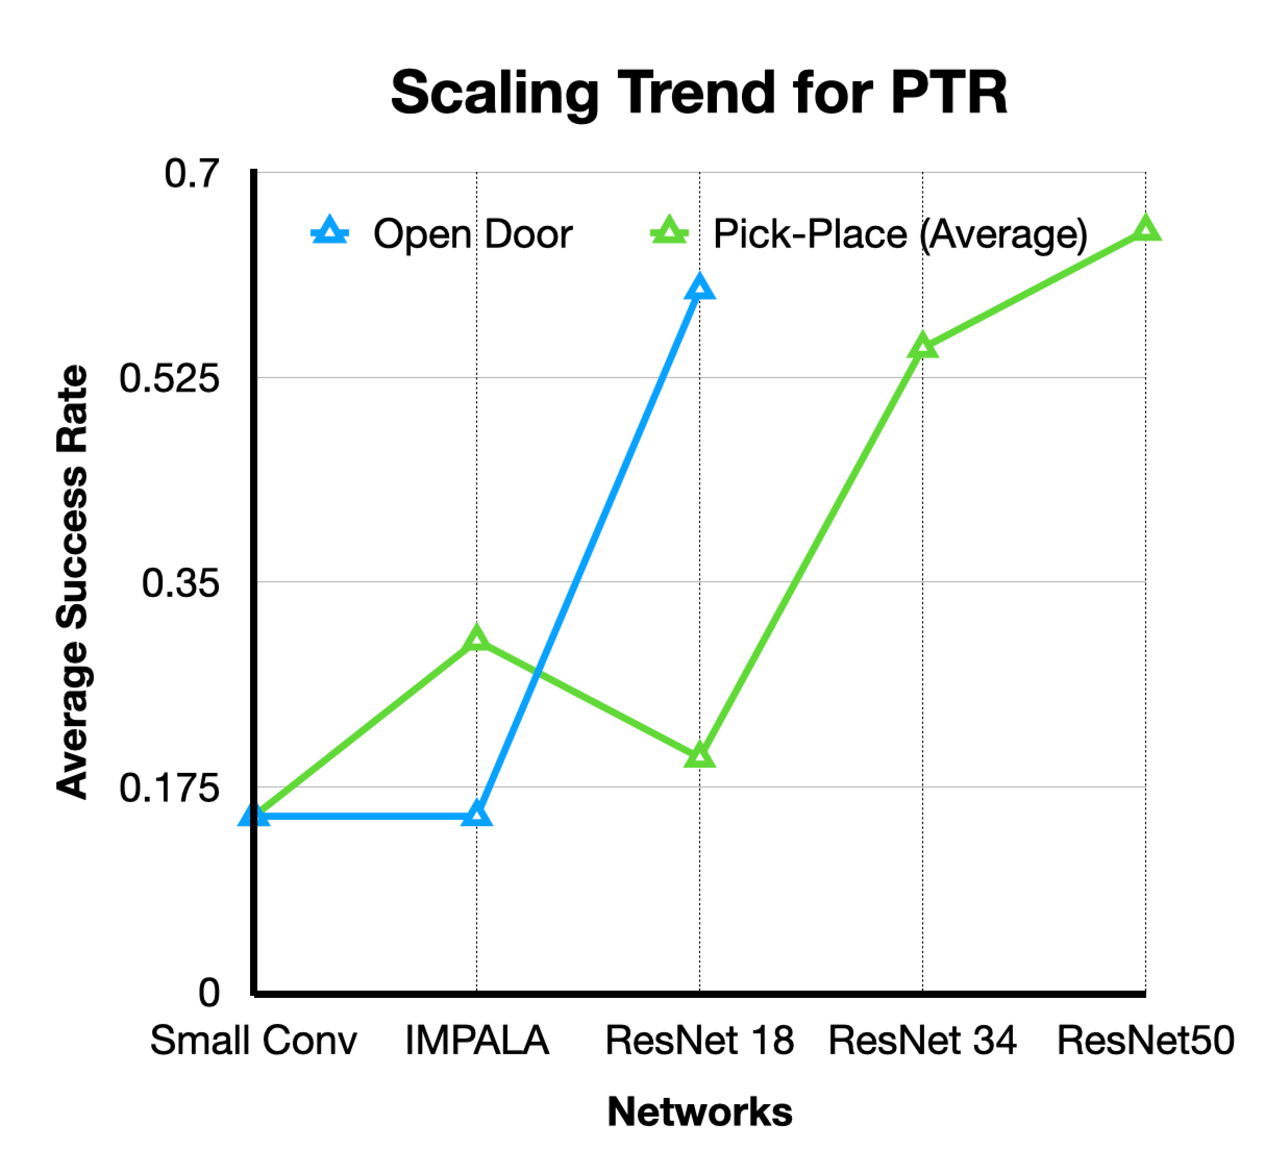
\includegraphics[width=0.9\linewidth]{scaling_ptr.pdf}
% \vspace{-0.1cm}
\caption{\footnotesize{\label{fig:scaling_ptr2} \textbf{Scaling trends for \methodname} on the open door task from Scenario 2, and average over two pick and place tasks (take croissant out of the metallic pot and put cucumber in the bowl) from Scenario 3. Note that more high capacity and expressive function approximators lead to the best results.}}
% \vspace{-0.6cm}
\end{figure}

\textbf{Highly expressive Q-networks are essential for good performance.} To assess the importance of highly expressive Q-functions, we evaluate the performance of \methodname with varying sizes and architectures on three tasks: the open door task from Scenario 2, and the put cucumber in the pot and take croissant out of metallic bowl tasks from Scenario 3. Our choice of architectures is as follows: \textbf{(a)} a standard three-layer convolutional network typically used by prior work for DM-control tasks (see for example, \citet{kostrikov2021offline}), \textbf{(b)} an IMPALA~\citep{espeholt2018impala} ResNet that consists of 15 convolutional layers spread across a stack of 3 residual blocks, \textbf{(c)} ResNet 18 with group normalization and learned spatial embeddings, \textbf{(d)} ResNet 34 that we use in our experiments, and \textbf{(e)} an even bigger ResNet 50 with group normalization and learned spatial embeddings. 

We present our results in {Figure~\ref{fig:scaling_ptr}}. To obtain more accurate scaling trends, we plot the trend in the average success rates for the pick and place tasks from Scenario 3 along with the trend in the success rate for the open door task separately since these tasks use different pre-training datasets. Observe that the performance of smaller networks (Small, IMPALA) is significantly worse than the ResNet in the door-opening task. For the pick and place tasks that contain a much larger dataset, Small, IMPALA, and ResNet18 all perform much worse than ResNet 34 and ResNet 50. We believe this result is quite exciting since it highlights the possibility of actually benefitting from using highly-expressive neural network models with TD-learning based RL methods trained on lots of diverse multi-task data (contrary to prior work~\citep{lee2022multi}). We believe that this result is a valuable starting point for further scaling and innovation.


\textbf{Learned spatial embeddings are crucial for performance.} Next we study the impact of utilizing the learned spatial embeddings for encoding spatial information when converting the feature maps from the convolutional stack into a vector that is fed into the fully-connected part of the Q-function. We compare our choice to utilizing a spatial softmax as in \citet{ebert2021bridge}, and also global average pooling (GAP) that simply averages over the spatial information, typically utilized in supervised learning with ResNets.


\begin{table}[h]
% \small{
\centering
% \vspace*{0.1cm}
\begin{tabular}{l|r}
\toprule
\textbf{Method} & \textbf{Success rate}\\  \midrule
PTR with spatial softmax & 4/10 \\
PTR with global average pooling & 4/10 \\
\midrule
PTR with learned spatial embeddings \textbf{(Ours)} & \textbf{7/10} \\
\bottomrule
\end{tabular}
\vspace{0.1cm}
\caption{\footnotesize{\textbf{Ablation of \methodname with spatial softmax and GAP on the croissant task.} Observe that \methodname with learned spatial embeddings performs significantly better than using a spatial softmax or global average pooling.}}
\label{tab:spatial}
\end{table}

As shown in {Table~\ref{tab:spatial}} learned spatial embeddings outperform both of these prior approaches on the put croissant in pot task. We suspect that spatial softmax does not perform much better than the GAP approach since the softmax operation can easily get saturated when running gradient descent to fit value targets that are not centered in some range, which would effectively hinder its expressivity. This indicates that the approach of retaining spatial information like in \methodname is required for attaining good performance.

\textbf{Concatenating actions at each layer is crucial for performance.} Next, we run \methodname without passing in actions at each fully connected layer of the Q-function on the take croissant out of metallic bowl task and only directly concatenate the actions with the output of the convolutional layers before passing it into the fully-connected component of the network. On the croissant task, we find that not passing in actions at each layer only succeeds in \textbf{2/10} evaluation rollouts, which is significantly worse than the default \methodname which passes in actions at each layer and succeeds in \textbf{7/10} evaluation rollouts (Table~\ref{tab:action_sep}).

\begin{table}[h]
% \small{
\centering
% \vspace*{0.1cm}
\begin{tabular}{l|r}
\toprule
\textbf{Method} & \textbf{Success rate}\\  \midrule
PTR without actions passed in at each FC layer & 2/10 \\
PTR with actions passed in at each FC layer (Ours) & \textbf{7/10} \\
\bottomrule
\end{tabular}
\vspace{0.1cm}
\caption{\footnotesize{\textbf{Ablation of \methodname with actions passed in at each layer.} Observe that passing in actions at each fully-connected layer does lead to quite good performance.}}
\label{tab:action_sep}
% \vspace{-0.5cm}
\end{table}

\textbf{Group normalization is more consistent than batch normalization.} Next, we ablate the usage of group normalization over batch normalization in the ResNet 34 Q-functions that \methodname uses. We found that batch normalization was generally harder to train to attain Q-function plots that exhibit a roughly increasing trend over the course of a trajectory. That said, on some tasks such as the croissant in pot task, we did get a reasonable Q-function, and found that batch normalization can perform well. On the other hand, on the put cucumber in pot task, we found that batch normalization was really ineffective. These results are shown in {Table~\ref{tab:batch_norm}}, and they demonstrate that batch normalization may not be as consistent and reliable with \methodname as group normalization.

\begin{table}
\centering
\scalebox{0.75}{
\begin{tabular}{l|r|r}
\toprule
\textbf{Method} & \textbf{Croissant out of metallic bowl} & \textbf{Cucumber in pot} \\  \midrule
PTR with batch norm. (relative) & + 28.0\% (7/10 $\rightarrow$ 9/10)& - 60.0\% (5/10 $\rightarrow$ 2/10) \\
\bottomrule
\end{tabular}
}
\vspace{0.1cm}
\caption{\footnotesize{\textbf{Relative performance of \methodname with batch normalization with respect to \methodname with group normalization.} Observe that while utilizing batch normalization in \methodname can be sometimes more effective than using group normalization (e.g., take croissant out of metallic bowl task), it may also be highly ineffective and can reduce success rates significantly in other tasks. The performance numbers to the left of the $\rightarrow$ correspond to the performance of \methodname with group normalization and the performance to the right of $\rightarrow$ is the performance with batch normalization.}}
\label{tab:batch_norm}
% \vspace{-0.5cm}
\end{table}


\textbf{Choice of the reward function.} Finally, we present some results that ablate the choice of the reward function utilized for training \methodname from data that entirely consists of demonstrations. In our main set of experiments, we labeled the last three timesteps of every trajectory with a reward of +1 and annotated all other timesteps with a 0 reward. We tried perhaps the most natural choice of labeling only the last timestep with a 0 reward on the croissant task and found that this choice succeeds \textbf{0/10} times, compared to annotating the last three timesteps with a +1 reward which succeeds \textbf{7/10} times. We suspect that this is because only annotating the last timestep with a +1 reward is not ideal for two reasons: first, the task is often completed in the dataset much earlier than the observation shows the task complete, and hence the last-step annotation procedure induces a non-Markovian reward function, and second, only labeling the last step with a +1 leads to overly conservative Q-functions when used with \methodname, which may not lead to good policies.

\subsection{More Details on Online Fine-tuning}
\label{app:online_finetuning}

\textbf{Offline pre-training.}
For both PTR and BC baseline, we used 40 open-door demonstrations as target task data and combined them with the Bridge Dataset to pre-train the policy. To reduce the training time in the real system, we used ResNet 18 backbones.

\textbf{Reset policy.}
For the reset policy, we additionally collected 22 close-door demonstrations as the target task data and pre-trained the policy with PTR. Similar to the open-door policy, we used ResNet 18 backbones to save training time.

\textbf{Reward classifier.} We used a ResNet 34 classification model and trained it to detect whether the door is open or closed from visual inputs. For the training data, we manipulated the robot to collect around 20 positive and negative trajectories for both open and closed doors.

\textbf{Method.} As shown by \citet{nakamoto2023calql} in simulation, offline value function initializations that learn conservative Q-functions may not be effective at fine-tuning if the learned Q-values are not at the same scale as the ground-truth return of the behavior policy. While this property does not affect offline performance, it is crucial to enforce this property during fine-tuning. That said, this property can be ``baked in'' by simply preventing the CQL regularizer from minimizing the learned Q-function if its values fall below the Monte-Carlo return of the trajectories in the dataset. Therefore, for the online fine-tuning experiment, we incorporate this constraint into PTR.

\textbf{Hyperparameters.} 
For both online fine-tuning with \methodname and SACfD, we performed the experiment by mixing the Bridge Dataset, offline target data, and the online data in a ratio ($\beta$) of 0.35, 0.15, and 0.5. For \methodname, we used the CQL alpha value of 5 for the offline phase and 0.5 for the online phase. 

\textbf{Evaluation.} The results shown in Figure~\ref{fig:online_door} were evaluated autonomously every 5K environment step during the online fine-tuning. Each evaluation was assessed with 10 trials, one from each initial position. The results shown in Figure~\ref{tab:online-finetune} were additionally evaluated over 3 trials from each initial position, using the offline initialization and the final checkpoint obtained after 20K environment steps of online fine-tuning.

\begin{figure}
% \vspace{-1cm}
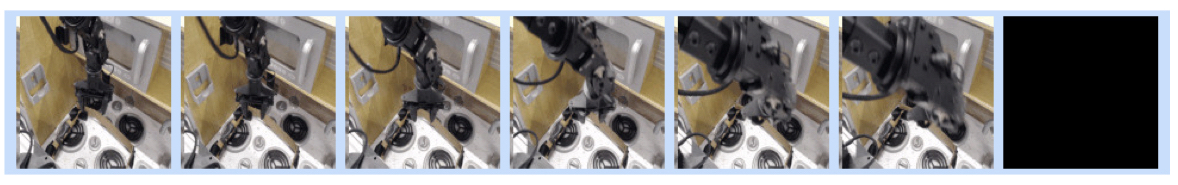
\includegraphics[width=\linewidth]{dangerous_actions.jpeg}
% \vspace{-0.1cm}
\caption{\footnotesize{\label{fig:dangerous-actions} \textbf{Example of unsafe behaviors when running SACfD.} The robot collides with the camera during online exploration, resulting in a system crash.}}
% \vspace{-0.6cm}
\end{figure}

\end{document}


